% =====================================================================
% Capítulo de resultados (abnTeX2). Incluir no documento principal com
% % =====================================================================
% Capítulo de resultados (abnTeX2). Incluir no documento principal com
% % =====================================================================
% Capítulo de resultados (abnTeX2). Incluir no documento principal com
% % =====================================================================
% Capítulo de resultados (abnTeX2). Incluir no documento principal com
% \include{resultados}. As figuras estão em figures/ (PDF vetorial; o PNG
% de mesmo nome serve para visualização).
%
% Estrutura (NBR 14724): o capítulo abre com as condições dos ensaios,
% segue a ordem dos casos de uso definidos na metodologia, cita cada
% figura e tabela no texto antes de ela aparecer, traz o título acima e a
% fonte abaixo, e discute cada resultado logo depois de apresentá-lo.
%
% Trechos marcados com "CONFERIR" dependem de informação que só o autor
% tem (condições dos ensaios). Revise antes de entregar.
%
% PROVISÓRIO: a janela de batimentos de 16/10 00:03 (caso de uso 2) tem
% valores fictícios. Substituir pela medição real antes da entrega.
% =====================================================================

\chapter{Resultados e discussão}
\label{cap:resultados}

Este capítulo apresenta os resultados obtidos com o protótipo entre 29 de setembro e 17 de outubro de 2026, organizados pelos casos de uso definidos na metodologia: localização (caso de uso 1), coleta biométrica (caso de uso 2), detecção de padrões repetitivos de movimento (caso de uso 3) e o caso de uso 4, ainda em andamento. Os dados foram extraídos da API do portal, a mesma que alimenta as telas do sistema, e processados por \textit{scripts} em Python para gerar as figuras.

Os ensaios foram feitos com o protótipo fora do animal: o sensor ficou sobre a bancada na maior parte do tempo e foi movimentado à mão nos testes de padrões, e a \textit{tag} de localização permaneceu em área urbana. % CONFERIR: condições dos ensaios
A Tabela~\ref{tab:condicoes} resume a configuração usada.

\begin{table}[htb]
  \centering
  \caption{Configuração do protótipo durante os ensaios}
  \label{tab:condicoes}
  \begin{tabular}{lp{8.5cm}}
    \hline
    \textbf{Item} & \textbf{Valor} \\
    \hline
    Microcontrolador & ESP32 DevKit \\
    Acelerômetro e giroscópio & MPU6050, 50 leituras/s \\
    Frequência cardíaca & MAX30102, 25 leituras/s \\
    Temperatura & DHT11, uma leitura a cada 20 s \\
    Armazenamento local & cartão microSD \\
    Intervalo de envio ao servidor & 180 s \\
    Localização & \textit{tag} BLE na rede Google Find Hub, consulta a cada 10 min \\
    Cerca virtual & círculo de 310 m de raio \\
    Período analisado & localização: 29/09 a 17/10/2026; sensor: 10/10 a 16/10/2026 \\
    \hline
  \end{tabular}
  \fonte{Elaborado pelo autor (2026).}
\end{table}

% ---------------------------------------------------------------------
\input{resultados_uc1}

% ---------------------------------------------------------------------
\section{Caso de uso 2: coleta biométrica}
\label{sec:res-biometria}

A Figura~\ref{fig:uc2-cobertura} mostra, para cada dia com o sensor ligado, quantos minutos têm leitura de cada sinal no servidor. O movimento somou 959 min e a temperatura 785 min. As leituras de frequência cardíaca somaram 304 s, distribuídos em oito janelas.

\begin{figure}[htb]
  \centering
  \caption{Minutos com leitura no servidor, por dia e por sinal}
  \label{fig:uc2-cobertura}
  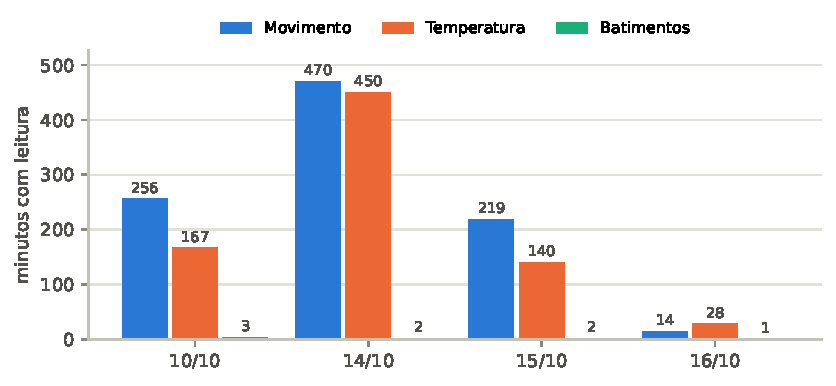
\includegraphics[width=0.95\linewidth]{figures/uc2_cobertura.pdf}
  \fonte{Elaborado pelo autor (2026).}
\end{figure}

A incerteza de cada sinal seguiu o mesmo procedimento do caso de uso 1 \cite{moffat1988}. A ordem zero é a metade da resolução do valor recebido \cite{poiate}; a primeira ordem é $2S$, com $S$ medido em um experimento auxiliar com o sensor em condição estável; o erro fixo vem da folha de dados ou de uma medição com valor conhecido; e a ordem $N$ é a soma quadrática dessas parcelas, a 95\% de confiança. A Tabela~\ref{tab:uc2-incerteza} resume os valores.

\begin{table}[htb]
  \centering
  \caption{Incerteza dos sinais biométricos a 95\% de confiança}
  \label{tab:uc2-incerteza}
  \begin{tabular}{lrrrr}
    \hline
    \textbf{Sinal} & \textbf{Ordem zero} & \textbf{1.ª ordem} & \textbf{Erro fixo} & \textbf{Ordem $N$} \\
    \hline
    Temperatura & 0,05 °C & 0,6 °C & 2,0 °C & 2,1 °C \\
    Movimento (minuto) & 0,00003 $g$ & 0,003 $g$ & 0,076 $g$ & 0,003 $g$\textsuperscript{a} \\
    Um batimento & 3,5 bpm & 6,0 bpm & não avaliado & 6,0 bpm \\
    Média de 16/10 & --- & 0,7 bpm & não avaliado & 0,7 bpm \\
    \hline
  \end{tabular}
  \fonte{Elaborado pelo autor (2026). \textsuperscript{a}Após descontar o erro fixo.}
\end{table}

\subsection{Frequência cardíaca}

O MAX30102 só calcula batimentos com pele encostada no sensor, e nos ensaios ele foi usado com o dedo do autor por poucos segundos. % CONFERIR
A Tabela~\ref{tab:bpm} lista as oito janelas. O sensor lê 25 vezes por segundo, e o intervalo entre dois picos tem resolução de 1/25 s. Pela propagação de $f = 60/T$, uma resolução $\delta T$ no período gera $\delta f = 60\,\delta T/T^2$ na frequência \cite{poiate}, valor que cresce com o quadrado da frequência: 3,5 bpm a 72 bpm e 21 bpm a 177 bpm.
% PROVISÓRIO: a janela de 16/10 00:03 tem valores fictícios (uc2.py, JANELA_PROVISORIA). Substituir pela medição real antes da entrega.

\begin{table}[htb]
  \centering
  \caption{Janelas com leitura de frequência cardíaca (bpm)}
  \label{tab:bpm}
  \begin{tabular}{lrrrrr}
    \hline
    \textbf{Início} & \textbf{Duração (s)} & \textbf{Média} & \textbf{Mínimo} & \textbf{Máximo} & \textbf{Resolução} \\
    \hline
    10/10 19:27 & 31 & 60,2 & 28,1 & 106,8 & 2,4 \\
    10/10 19:27 & 9 & 51,0 & 27,1 & 76,3 & 1,7 \\
    10/10 19:28 & 57 & 62,4 & 34,1 & 79,7 & 2,6 \\
    14/10 18:07 & 29 & 62,7 & 23,0 & 75,7 & 2,6 \\
    14/10 21:12 & 55 & 53,6 & 21,7 & 105,3 & 1,9 \\
    15/10 20:34 & 8 & 78,5 & 34,2 & 177,0 & 4,1 \\
    15/10 23:54 & 55 & 67,0 & 31,0 & 176,5 & 3,0 \\
    16/10 00:03 & 60 & 72,5 & 68,2 & 78,9 & 3,5 \\ % PROVISÓRIO
    \hline
  \end{tabular}
  \fonte{Elaborado pelo autor (2026). Resolução de um batimento na frequência média da janela.}
\end{table}

Nas sete primeiras janelas, os mínimos (22 a 34 bpm) e os máximos (até 177 bpm) se afastam da média muito mais que a resolução, o que mostra que o algoritmo de detecção de pulso aceitou picos falsos quando o dedo se moveu. O sensor dividia o barramento I2C com o MPU6050 em fios sem solda, e as falhas de contato desligaram a leitura de batimentos em parte do período. Na janela de 16/10, com 60 s de contato contínuo, a Figura~\ref{fig:uc2-batimentos} mostra os 73 batimentos. A média foi de $(72{,}5 \pm 0{,}7)$~bpm, com $S = 3{,}0$~bpm e $t = 1{,}99$ para 72 graus de liberdade, e a incerteza de um batimento isolado foi de $\pm 6{,}0$~bpm. Os valores se repetem em 68,2, 71,4, 75,0 e 78,9 bpm porque o período é contado em passos de 40 ms, e a resolução responde por boa parte da dispersão. O erro fixo do sensor exige comparação com um oxímetro de referência e não foi avaliado. % CONFERIR

\begin{figure}[htb]
  \centering
  \caption{Frequência de cada batimento na janela de 16/10, com a incerteza da média e de um batimento}
  \label{fig:uc2-batimentos}
  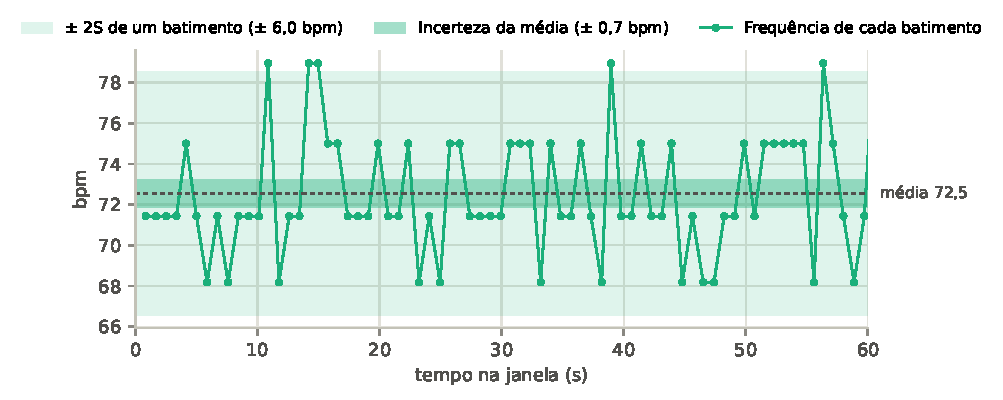
\includegraphics[width=0.95\linewidth]{figures/uc2_batimentos.pdf}
  \fonte{Elaborado pelo autor (2026).}
\end{figure}

\subsection{Temperatura}

A Figura~\ref{fig:uc2-temperatura} apresenta a temperatura como o portal a exibe, com a faixa de incerteza e os limites de alerta (35~°C e 40~°C) em vermelho. No dia 14/10 o DHT11 mediu o ar da sala, entre 24,0~°C e 27,9~°C em 450 leituras. A primeira ordem foi obtida das diferenças entre leituras sucessivas desse dia, que retiram a variação lenta da sala: $S = 0{,}30$~°C. A folha de dados do DHT11 informa exatidão de $\pm 2$~°C, adotada como erro fixo a 95\%. A ordem $N$ ficou em 2,1~°C, dominada pelo erro fixo.

\begin{figure}[htb]
  \centering
  \caption{Temperatura medida, incerteza e limites de alerta com as zonas de dúvida}
  \label{fig:uc2-temperatura}
  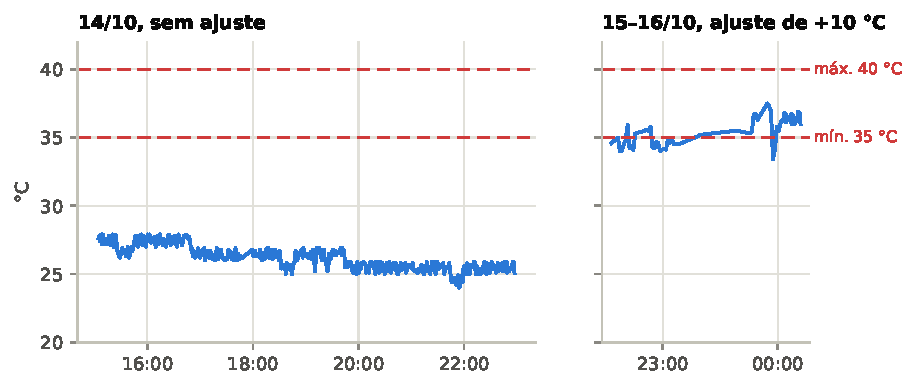
\includegraphics[width=0.95\linewidth]{figures/uc2_temperatura.pdf}
  \fonte{Elaborado pelo autor (2026).}
\end{figure}

Os limites de alerta formam uma tolerância de 5~°C. Pelo critério de \citeonline{poiate}, a incerteza deveria ficar abaixo de um décimo desse intervalo, 0,5~°C, e a do DHT11 é quatro vezes maior. A zona de aceitação fica reduzida a 37,1~°C a 37,9~°C, e as faixas de 32,9~°C a 37,1~°C e de 37,9~°C a 42,1~°C são zonas de dúvida, em que a medição não permite afirmar se a temperatura está dentro ou fora dos limites. As 450 leituras de 14/10 ficaram na zona de rejeição, abaixo do mínimo. Na noite de 15/10 foi salvo no portal um ajuste de +10~°C, usado para testar o caminho da calibração e não como correção medida. % CONFERIR
O sensor baixou o ajuste no envio seguinte e, a partir das 23h, as leituras passaram para a faixa de 33,4~°C a 37,5~°C: 47 das 49 leituras caíram na zona de dúvida e duas na zona de aceitação.

O teste confirma que o ajuste feito no portal chega ao sensor sem regravar o \textit{firmware} e passa a valer na comparação com os limites. O valor de +10~°C, porém, não corresponde a nenhuma referência e não reduz a incerteza: para uso no animal, o ajuste deve ser obtido comparando o sensor com um termômetro clínico, e um sensor com exatidão de 0,5~°C ou melhor atenderia ao critério de um décimo da tolerância.

\subsection{Movimento}

A Figura~\ref{fig:uc2-movimento} mostra a intensidade do movimento em 14/10, calculada como o afastamento do módulo da aceleração em relação a 1~$g$. Não havia limite de movimento configurado nesse dia. Nos 348 minutos com o sensor parado, a média por minuto foi de $(0{,}0761 \pm 0{,}0002)$~$g$, quando o esperado seria zero, com $S = 0{,}0016$~$g$ entre minutos. Nos 60 s mais estáveis das leituras brutas de 15/10, a 50 leituras/s, o módulo médio foi de 1,077~$g$, com $S = 0{,}003$~$g$ por leitura. O desvio de 0,076~$g$ é um erro fixo de escala do MPU6050, de 7,7\%, e é o motivo de o portal oferecer o ganho de calibração do movimento: com o ganho de $1/1{,}077$, a incerteza restante por minuto cai para 0,003~$g$. Sem a correção, o erro fixo precisa entrar na incerteza \cite{moffat1988}, e valores abaixo de cerca de 0,08~$g$ não se distinguem do sensor parado. Os picos de até 2,36~$g$ correspondem aos momentos em que o sensor foi manuseado e superam essa faixa com folga.

\begin{figure}[htb]
  \centering
  \caption{Intensidade do movimento por minuto em 14/10, com o erro fixo medido com o sensor parado (escala logarítmica acima de 0,1~$g$)}
  \label{fig:uc2-movimento}
  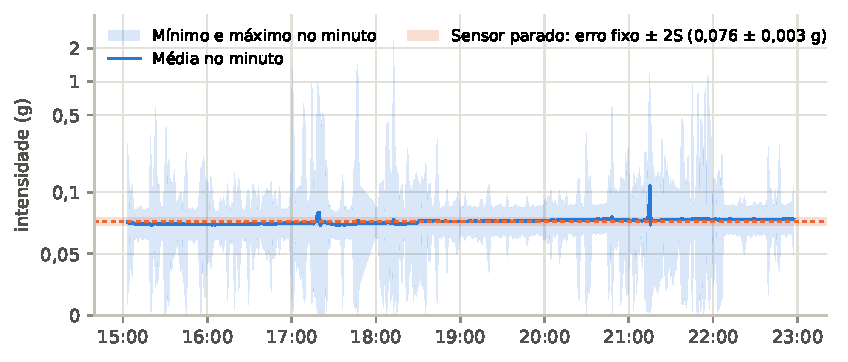
\includegraphics[width=0.95\linewidth]{figures/uc2_movimento.pdf}
  \fonte{Elaborado pelo autor (2026).}
\end{figure}

O envio de alertas por e-mail ao veterinário não foi avaliado, pois o servidor de e-mail (SMTP) não estava configurado no período. Os alertas pelo LED do sensor e pelo sino do portal foram verificados de forma visual, sem registro quantitativo. % CONFERIR

% ---------------------------------------------------------------------
\section{Caso de uso 3: detecção de padrões repetitivos}
\label{sec:res-padroes}

Os padrões ``Pulo'' e ``Volta'' foram avaliados em uma sessão de testes em 15/10, com 87,7 min de leituras do acelerômetro (263.089 amostras a 50 Hz). Nessa sessão o autor marcou no portal dez trechos, oito de Pulo e dois de Volta, que somam 22 s. Duas versões de detecção rodaram no sensor: até as 23h05, o modelo supervisionado treinado no servidor (floresta de 15 árvores de profundidade 4); depois desse horário, o detector físico descrito na metodologia.

A Figura~\ref{fig:uc3-sinal} mostra um trecho de 35 s com os três eixos, a marcação feita no portal (faixa cinza) e os eventos que o sensor registrou com o modelo supervisionado (linhas tracejadas).

\begin{figure}[htb]
  \centering
  \caption{Sinal do acelerômetro, trecho marcado como Pulo e eventos registrados pelo sensor}
  \label{fig:uc3-sinal}
  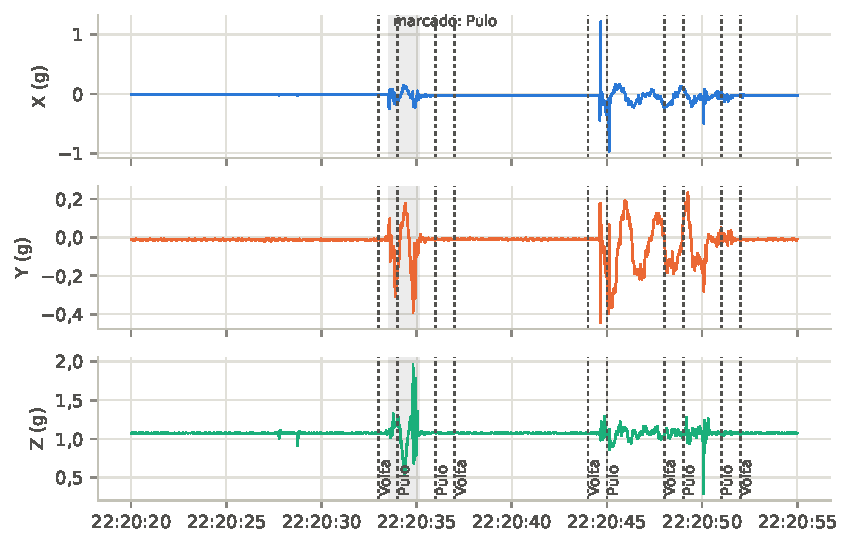
\includegraphics[width=0.95\linewidth]{figures/uc3_sinal_marcacoes.pdf}
  \fonte{Elaborado pelo autor (2026).}
\end{figure}

No trecho marcado, o eixo Z cai até cerca de 0,6~$g$ e sobe a quase 2~$g$, e o sensor registrou um Pulo dentro da marcação. O modelo, porém, também registrou eventos de Volta no mesmo instante e Pulos durante o manuseio seguinte, que não foi marcado. A Figura~\ref{fig:uc3-modelo} apresenta o desempenho do modelo supervisionado na validação feita pelo servidor no treino, deixando uma marcação de fora de cada vez.

\begin{figure}[htb]
  \centering
  \caption{Desempenho do modelo supervisionado na validação do treino}
  \label{fig:uc3-modelo}
  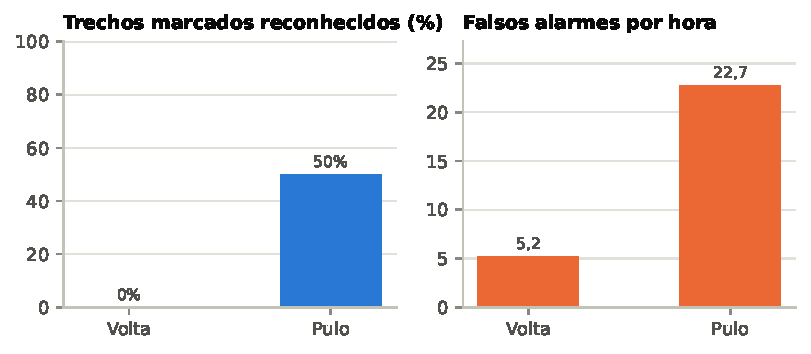
\includegraphics[width=0.95\linewidth]{figures/uc3_modelo_supervisionado.pdf}
  \fonte{Elaborado pelo autor (2026).}
\end{figure}

O modelo reconheceu 50\% dos trechos de Pulo, com 22,7 falsos alarmes por hora fora das marcações, e nenhum trecho de Volta. Com oito exemplos de Pulo (31 janelas) contra 3.000 janelas negativas, e dois exemplos de Volta, a base de treino é pequena demais para separar os padrões do manuseio comum do sensor. Esse resultado levou à troca do modelo supervisionado por um detector baseado na física do movimento, que não depende de exemplos marcados.

No detector físico, um salto é identificado pelo tempo $T$ em queda livre, em que o módulo da aceleração fica abaixo de 0,6~$g$. A altura vem da equação do lançamento vertical, $h = gT^2/8$, e o salto só é contado acima de 5~cm. A Figura~\ref{fig:uc3-voo} mostra os 20 voos com pelo menos 0,06 s encontrados ao reaplicar essa regra às leituras da sessão.

\begin{figure}[htb]
  \centering
  \caption{Altura estimada de cada voo pelo tempo em queda livre e limiar de contagem}
  \label{fig:uc3-voo}
  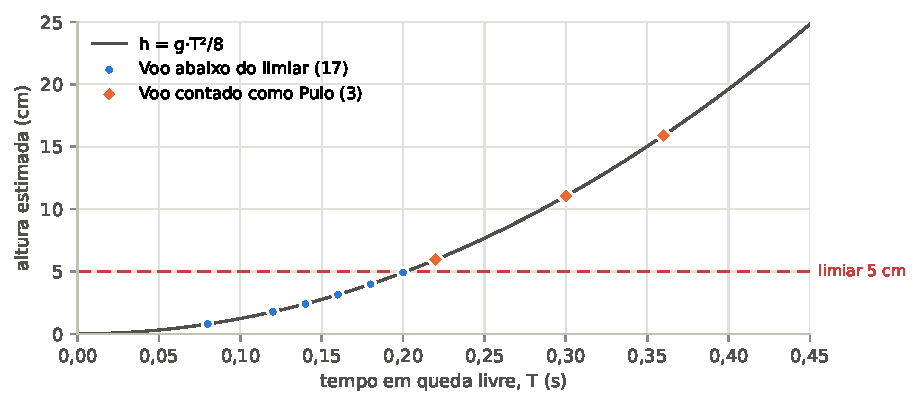
\includegraphics[width=0.95\linewidth]{figures/uc3_voo_altura.pdf}
  \fonte{Elaborado pelo autor (2026).}
\end{figure}

Três voos passaram do limiar, com 5,9 cm, 11 cm e 15,9 cm; os outros 17 ficaram entre 0,8 cm e 4,9 cm. Os oito trechos marcados como Pulo tiveram voos abaixo de 5 cm, de modo que nenhum deles foi contado. Os saltos do teste foram pequenos, feitos levantando e soltando a placa, e ficaram na faixa em que a regra não distingue um salto de um solavanco. Em um cavalo, um salto de 1 m corresponde a cerca de 0,9 s em queda livre, valor muito acima do ruído observado.

A Tabela~\ref{tab:uc3} compara as duas versões. A versão supervisionada é a que rodou no sensor até as 23h05; a física foi reaplicada às leituras da sessão inteira. Os eventos fora das marcações não equivalem a falsos alarmes, pois o autor não marcou todos os movimentos feitos durante a sessão.

\begin{table}[htb]
  \centering
  \caption{Marcações reconhecidas e eventos por versão de detecção na sessão de 15/10}
  \label{tab:uc3}
  \begin{tabular}{llrrr}
    \hline
    \textbf{Padrão} & \textbf{Versão} & \textbf{Marcações} & \textbf{Reconhecidas} & \textbf{Eventos} \\
    \hline
    Pulo  & Supervisionada (sensor) & 6 & 1 & 39 \\
    Volta & Supervisionada (sensor) & 2 & 0 & 42 \\
    Pulo  & Física (reaplicada) & 8 & 0 & 3 \\
    Volta & Física (reaplicada) & 2 & 2 & 22 \\
    \hline
  \end{tabular}
  \fonte{Elaborado pelo autor (2026).}
\end{table}

Para a Volta, o detector físico reconheceu os dois trechos marcados ao somar 360° de rotação do vetor horizontal da aceleração, e registrou 22 voltas na sessão, contra 42 do modelo supervisionado em um período menor. A reaplicação usou apenas o método do vetor horizontal, pois as leituras do giroscópio não ficam guardadas no servidor; no sensor, a volta também é contada pela rotação medida pelo giroscópio.

% ---------------------------------------------------------------------
\section{Caso de uso 4}
\label{sec:res-uc4}

% PENDENTE: resultados do caso de uso 4.
Os resultados deste caso de uso serão apresentados após a conclusão dos ensaios.

% ---------------------------------------------------------------------
\section{Síntese dos resultados}
\label{sec:res-sintese}

O protótipo coletou e enviou ao servidor 959 min de movimento e 785 min de temperatura em quatro dias, com as leituras guardadas no cartão SD entre um envio e outro. A localização pela rede Find Hub detectou a saída da cerca em 30/09, com posições a cada 16 min (mediana) e incerteza de 19 m (leste) e 28 m (norte) a 95\% de confiança. Com essa incerteza, o site soma cerca de 14 m por passo com a \textit{tag} parada, e a distância só foi significativa no dia com deslocamento. A calibração e os limites definidos no portal chegaram ao sensor sem regravar o \textit{firmware}. A frequência cardíaca teve 304 s de leitura, limitada pelo contato com a pele e pelas conexões do barramento I2C, e a janela com contato contínuo deu $(72{,}5 \pm 0{,}7)$~bpm. % PROVISÓRIO: valor da janela fictícia de 16/10
A temperatura teve incerteza de 2,1~°C, quatro vezes o recomendado para os limites de alerta, e o movimento, um erro fixo de 0,076~$g$ que o ganho de calibração corrige. Na detecção de padrões, o modelo supervisionado não atingiu desempenho útil com dez marcações, e o detector físico reconheceu as voltas marcadas, mas os saltos de teste ficaram abaixo do limiar de 5 cm. Os ensaios no animal são a próxima etapa para medir esses valores em condições reais.
. As figuras estão em figures/ (PDF vetorial; o PNG
% de mesmo nome serve para visualização).
%
% Estrutura (NBR 14724): o capítulo abre com as condições dos ensaios,
% segue a ordem dos casos de uso definidos na metodologia, cita cada
% figura e tabela no texto antes de ela aparecer, traz o título acima e a
% fonte abaixo, e discute cada resultado logo depois de apresentá-lo.
%
% Trechos marcados com "CONFERIR" dependem de informação que só o autor
% tem (condições dos ensaios). Revise antes de entregar.
%
% PROVISÓRIO: a janela de batimentos de 16/10 00:03 (caso de uso 2) tem
% valores fictícios. Substituir pela medição real antes da entrega.
% =====================================================================

\chapter{Resultados e discussão}
\label{cap:resultados}

Este capítulo apresenta os resultados obtidos com o protótipo entre 29 de setembro e 17 de outubro de 2026, organizados pelos casos de uso definidos na metodologia: localização (caso de uso 1), coleta biométrica (caso de uso 2), detecção de padrões repetitivos de movimento (caso de uso 3) e o caso de uso 4, ainda em andamento. Os dados foram extraídos da API do portal, a mesma que alimenta as telas do sistema, e processados por \textit{scripts} em Python para gerar as figuras.

Os ensaios foram feitos com o protótipo fora do animal: o sensor ficou sobre a bancada na maior parte do tempo e foi movimentado à mão nos testes de padrões, e a \textit{tag} de localização permaneceu em área urbana. % CONFERIR: condições dos ensaios
A Tabela~\ref{tab:condicoes} resume a configuração usada.

\begin{table}[htb]
  \centering
  \caption{Configuração do protótipo durante os ensaios}
  \label{tab:condicoes}
  \begin{tabular}{lp{8.5cm}}
    \hline
    \textbf{Item} & \textbf{Valor} \\
    \hline
    Microcontrolador & ESP32 DevKit \\
    Acelerômetro e giroscópio & MPU6050, 50 leituras/s \\
    Frequência cardíaca & MAX30102, 25 leituras/s \\
    Temperatura & DHT11, uma leitura a cada 20 s \\
    Armazenamento local & cartão microSD \\
    Intervalo de envio ao servidor & 180 s \\
    Localização & \textit{tag} BLE na rede Google Find Hub, consulta a cada 10 min \\
    Cerca virtual & círculo de 310 m de raio \\
    Período analisado & localização: 29/09 a 17/10/2026; sensor: 10/10 a 16/10/2026 \\
    \hline
  \end{tabular}
  \fonte{Elaborado pelo autor (2026).}
\end{table}

% ---------------------------------------------------------------------
% =====================================================================
% Caso de uso 1 (localização). Seção do capítulo de resultados, incluída
% em resultados.tex com \input{resultados_uc1}. Figuras em figuras/*.jpg.
% Incerteza: Moffat (1988) e Poiate Junior (apostila), chaves em referencias.bib.
% Trechos marcados com "CONFERIR" dependem de informação do autor.
% =====================================================================

\section{Caso de uso 1: localização}
\label{sec:res-localizacao}

O intervalo analisado vai de 29/09/2026 a 17/10/2026 e reúne 275 posições da \textit{tag}. As 32 primeiras, até 10/10, foram coletadas pela instância local do servidor, antes da implantação; as 243 seguintes, pela instância em produção. As duas instâncias usam o mesmo código de consulta e de filtragem. Entre 30/09 e 10/10 não há posições, porque o servidor local ficou desligado nesse período. % CONFERIR: motivo da lacuna
As posições estão em metros a partir do centro da cerca virtual, sem mapa de fundo, para não expor o endereço do local de teste.

A Figura~\ref{fig:uc1-trajeto} apresenta as posições em duas escalas. Em (a), o período de 10/10 a 17/10, com a \textit{tag} parada dentro da cerca de 310 m de raio. Em (b), o intervalo total, que inclui o deslocamento a pé feito pelo autor em 30/09.

\begin{figure}[htb]
  \centering
  \caption{Posições recebidas da \textit{tag} e cerca virtual: (a) período com a \textit{tag} parada; (b) intervalo total}
  \label{fig:uc1-trajeto}
  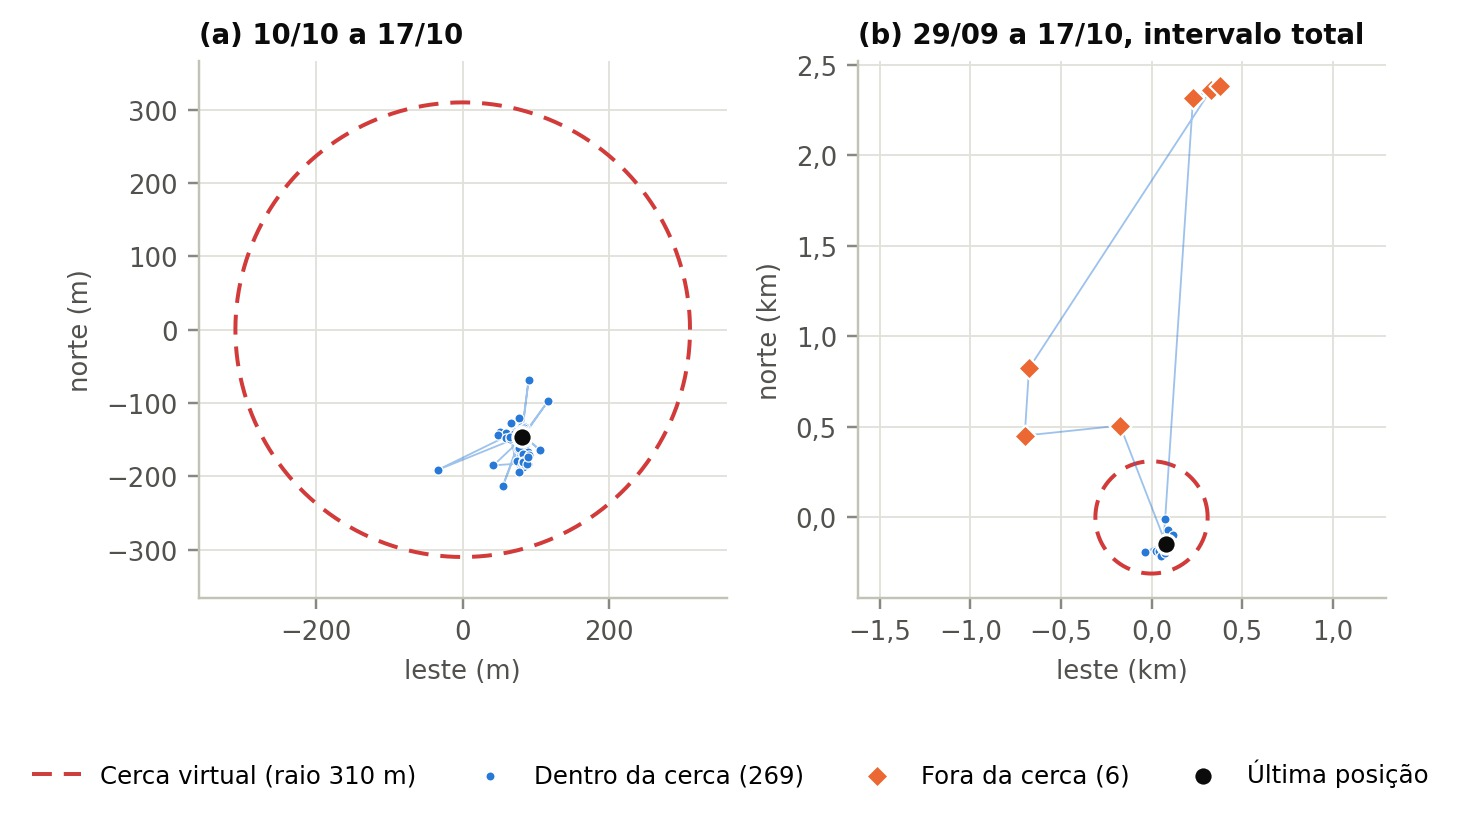
\includegraphics[width=\textwidth]{figuras/uc1_trajeto.jpg}
  \fonte{Elaborado pelo autor (2026).}
\end{figure}

Seis posições ficaram fora da cerca, todas em 30/09, entre 13h32 e 14h31, a até 2,41 km do centro. O site registrou o alerta de saída da cerca a partir da primeira delas: o cartão de localização do cavalo passou a indicar ``Fora da cerca'' e o alerta apareceu no sino do portal. Nas demais 269 posições a \textit{tag} estava dentro do raio.

A Figura~\ref{fig:uc1-dia} mostra quantas posições chegaram em cada dia. A quantidade variou de 6 a 75 por dia. A rede Find Hub depende de celulares Android que passem perto da \textit{tag}, e o servidor só registra o que a rede entrega.

\begin{figure}[htb]
  \centering
  \caption{Posições recebidas por dia, dentro e fora da cerca}
  \label{fig:uc1-dia}
  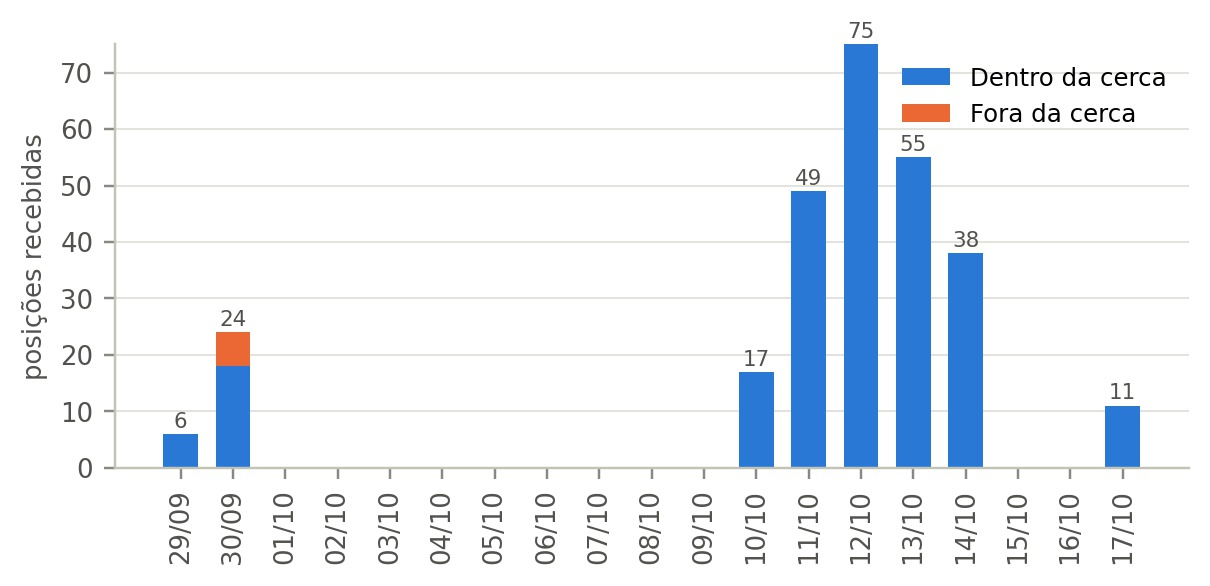
\includegraphics[width=\textwidth]{figuras/uc1_por_dia.jpg}
  \fonte{Elaborado pelo autor (2026).}
\end{figure}

A Figura~\ref{fig:uc1-intervalo} apresenta o intervalo entre posições consecutivas e a precisão informada pela rede em cada posição. O intervalo mediano foi de 16 min, e 90\% dos intervalos ficaram abaixo de 57 min; o maior intervalo, de 239 h, corresponde à lacuna entre 30/09 e 10/10. A precisão informada teve mediana de 75 m, e 46\% das posições chegaram com o valor máximo aceito pelo filtro do servidor, 100 m.

\begin{figure}[htb]
  \centering
  \caption{Intervalo entre posições consecutivas e precisão informada pela rede}
  \label{fig:uc1-intervalo}
  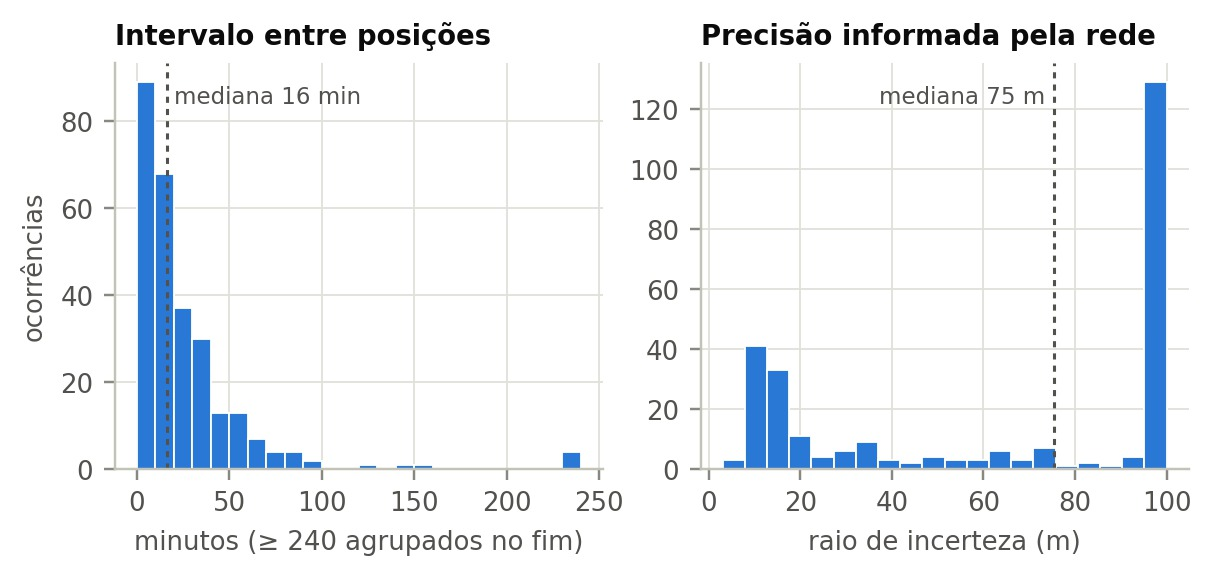
\includegraphics[width=\textwidth]{figuras/uc1_intervalo_precisao.jpg}
  \fonte{Elaborado pelo autor (2026).}
\end{figure}

\subsection{Incerteza da posição}
\label{sec:uc1-incerteza-posicao}

A incerteza foi avaliada pela análise de amostra única de \citeonline{moffat1988}: cada posição é uma leitura isolada, e a dispersão do sistema de medição é obtida de um experimento auxiliar feito em condição representativa. O experimento auxiliar foi o período de 10/10 a 17/10, com a \textit{tag} parada no mesmo ponto e 243 leituras. As coordenadas foram convertidas para metros nas direções leste ($x$) e norte ($y$), e o desvio-padrão amostral de cada direção foi $S_x = 9{,}6$~m e $S_y = 14{,}0$~m.

Com 242 graus de liberdade, a distribuição qui-quadrado limita o desvio-padrão da população a $0{,}92\,S \le \sigma \le 1{,}10\,S$, ao nível de 95\% \cite{moffat1988}. Foi adotado o valor mais provável, $\sigma = S$. A incerteza de uma leitura isolada, a 95\% de confiança (chance de 20 para 1), é
\begin{equation}
  \delta x = 2\sigma_x = 19{,}2~\text{m}, \qquad \delta y = 2\sigma_y = 27{,}9~\text{m}.
  \label{eq:uc1-incerteza-posicao}
\end{equation}
Com o limite superior de $\sigma$, os valores seriam 21,0 m e 30,6 m. Nos dados, 96,3\% das leituras ficaram dentro de $\pm\delta x$ e 92,2\% dentro de $\pm\delta y$. A distribuição não é gaussiana, pois 92\% das leituras na direção leste ficaram dentro de $\pm S_x$, e uma leitura isolada se afastou 121 m da média. A autocorrelação entre leituras consecutivas foi de $-0{,}001$ (leste) e $0{,}12$ (norte), e as leituras foram tratadas como independentes, condição exigida para a soma quadrática.

A Tabela~\ref{tab:uc1-ordens} separa a incerteza da posição nas três ordens de \citeonline{moffat1988}. A ordem zero corresponde à resolução dos valores recebidos, que chegam com $10^{-7}$ grau (cerca de 1,1 cm), e a incerteza instrumental é a metade da resolução \cite{poiate}. O horário de cada posição chega em segundos inteiros, com incerteza de 0,5 s. A primeira ordem é a dispersão medida no experimento auxiliar. Na ordem $N$ entraria o erro fixo da rede, isto é, a diferença entre a média das leituras e a posição verdadeira da \textit{tag}. Esse erro não foi medido, porque não havia uma referência de posição com incerteza menor; ele desloca todas as leituras da mesma forma, e por isso se cancela nas diferenças entre posições usadas na distância e na velocidade, mas afeta a verificação da cerca.

\begin{table}[htb]
  \centering
  \caption{Incerteza de uma posição a 95\% de confiança}
  \label{tab:uc1-ordens}
  \begin{tabular}{lrrl}
    \hline
    \textbf{Ordem} & \textbf{Leste (m)} & \textbf{Norte (m)} & \textbf{Origem} \\
    \hline
    Zero & 0,005 & 0,006 & resolução de $10^{-7}$ grau \\
    Primeira & 19,2 & 27,9 & experimento auxiliar, $2S$ \\
    $N$ & 19,2 & 27,9 & erro fixo da rede não avaliado \\
    \hline
  \end{tabular}
  \fonte{Elaborado pelo autor (2026).}
\end{table}

A ordem zero é cerca de 4 mil vezes menor que a primeira e foi desprezada, pois uma parcela menor que um terço da maior tem efeito pequeno na soma quadrática \cite{moffat1988}. Em 95,9\% das leituras paradas, a distância até a média ficou abaixo da precisão informada pela rede para aquela leitura, cuja mediana foi de 75 m. A precisão informada se comporta como um limite conservador, maior que a incerteza medida.

\subsection{Verificação da cerca com a incerteza}

A cerca virtual funciona como uma tolerância: a posição é aceita enquanto a distância $r$ até o centro não passa do raio $R = 310$~m. Seguindo \citeonline{poiate}, a incerteza de medição divide a faixa em três zonas. A zona de aceitação vai até $R - \delta r$, a zona de rejeição começa em $R + \delta r$ e, entre as duas, fica a zona de dúvida, onde a medição não permite afirmar se a \textit{tag} está dentro ou fora. A incerteza da distância ao centro vem da propagação das incertezas da Equação~\eqref{eq:uc1-incerteza-posicao}:
\begin{equation}
  \delta r = \sqrt{\left(\frac{x}{r}\,\delta x\right)^2 + \left(\frac{y}{r}\,\delta y\right)^2}.
  \label{eq:uc1-incerteza-raio}
\end{equation}

O maior valor de $\delta r$ entre as posições foi de 27,8 m, o que coloca a zona de dúvida entre 282 m e 338 m. A incerteza ficou abaixo de um décimo do intervalo de tolerância (31 m), critério de equilíbrio entre custo e qualidade recomendado por \citeonline{poiate}. A Figura~\ref{fig:uc1-zonas} mostra a distância de cada posição ao centro com as três zonas.

\begin{figure}[htb]
  \centering
  \caption{Distância das posições ao centro da cerca, com as zonas de aceitação, dúvida e rejeição}
  \label{fig:uc1-zonas}
  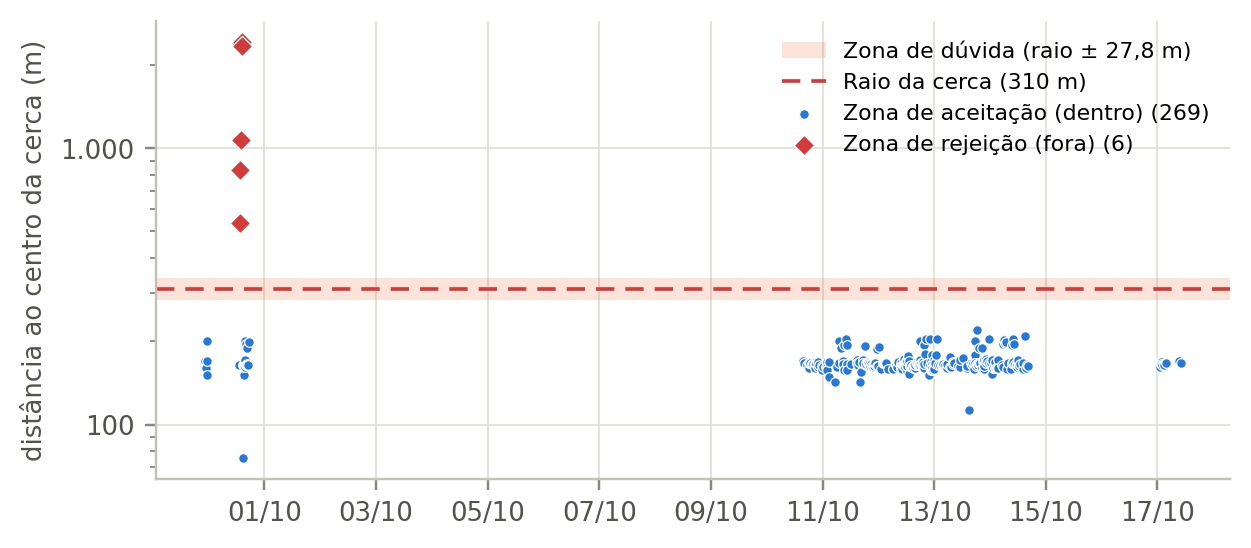
\includegraphics[width=\textwidth]{figuras/uc1_zonas.jpg}
  \fonte{Elaborado pelo autor (2026).}
\end{figure}

As 269 posições dentro da cerca ficaram a até 220 m do centro, na zona de aceitação. As seis posições de 30/09 ficaram a pelo menos 536 m, na zona de rejeição, e nenhuma posição caiu na zona de dúvida. O alerta de saída da cerca de 30/09 não depende, portanto, da incerteza da posição.

\subsection{Parâmetros calculados pelo site}

O site calcula, a partir das posições gravadas no banco, quatro parâmetros para o intervalo escolhido. A distância percorrida é a soma das distâncias entre posições consecutivas, $d = \sum_k s_k$. A velocidade média é essa distância dividida pelo tempo $T$ entre a primeira e a última posição. A velocidade máxima é a maior razão $s_k/\Delta t_k$ entre duas posições consecutivas. A aceleração média é a média das variações de velocidade entre trechos seguidos.

A incerteza desses resultados foi propagada pelo método da perturbação sequencial \cite{moffat1988}, aplicado à mesma função de cálculo do site. Cada entrada $X_i$ (latitude, longitude e horário de cada posição) foi aumentada e reduzida pela sua incerteza $\delta X_i$, uma de cada vez, e a contribuição $C_i$ foi tomada como a média de $|R_{i+} - R_0|$ e $|R_{i-} - R_0|$, porque o resultado não é linear nas posições. A incerteza do resultado é a soma quadrática das contribuições,
\begin{equation}
  \delta R = \sqrt{\sum_i C_i^2}, \qquad C_i \approx \frac{\partial R}{\partial X_i}\,\delta X_i,
  \label{eq:uc1-perturbacao}
\end{equation}
e tem o mesmo nível de confiança das entradas, 95\%. Para a velocidade média, a propagação analítica da apostila de \citeonline{poiate},
\begin{equation}
  \frac{\delta \bar v}{\bar v} = \sqrt{\left(\frac{\delta d}{d}\right)^2 + \left(\frac{\delta T}{T}\right)^2},
  \label{eq:uc1-vmed}
\end{equation}
com $\delta T = 1$~s (metade da resolução em cada extremo), deu o mesmo valor que a perturbação sequencial até a terceira casa. A parcela do horário foi desprezível em todos os resultados, exceto na velocidade máxima de 13/10, em que foi de 23 km/h contra 128 km/h da parcela das posições.

A soma de passos tem também um erro fixo, que \citeonline{moffat1988} classifica como erro conceitual: com a \textit{tag} parada, o ruído da posição gera passos de comprimento não nulo, e o site os soma como distância. Esse erro foi medido no experimento auxiliar, com 121 pares de leituras consecutivas sem leitura em comum. O passo médio foi de $(14{,}0 \pm 3{,}3)$~m, em que a incerteza é $t\,S/\sqrt{N}$, com $t = 1{,}98$ para 120 graus de liberdade. Para um intervalo com $k$ passos, o erro fixo é $B = k \times 14{,}0$~m, e a sua incerteza, $k \times 3{,}3$~m, somada de forma linear, porque o mesmo valor médio é usado em todos os passos. A distância corrigida é $d - B$, e a sua incerteza de ordem $N$ é a soma quadrática da incerteza propagada com a incerteza de $B$. Essa correção supõe a \textit{tag} parada em todos os passos e, nos dias com deslocamento, superestima o erro fixo. A velocidade média recebe a mesma correção, dividida por $T$.

A Figura~\ref{fig:uc1-parametros} apresenta, por dia, o valor calculado pelo site, a incerteza expandida e o erro fixo. Um valor foi considerado significativo quando superou a sua incerteza, isto é, quando a diferença em relação a zero (ou ao erro fixo, no caso da distância e da velocidade média) foi maior que a incerteza dessa diferença \cite{moffat1988}.

\begin{figure}[htb]
  \centering
  \caption{Parâmetros calculados pelo site por dia, com a incerteza expandida e o erro fixo}
  \label{fig:uc1-parametros}
  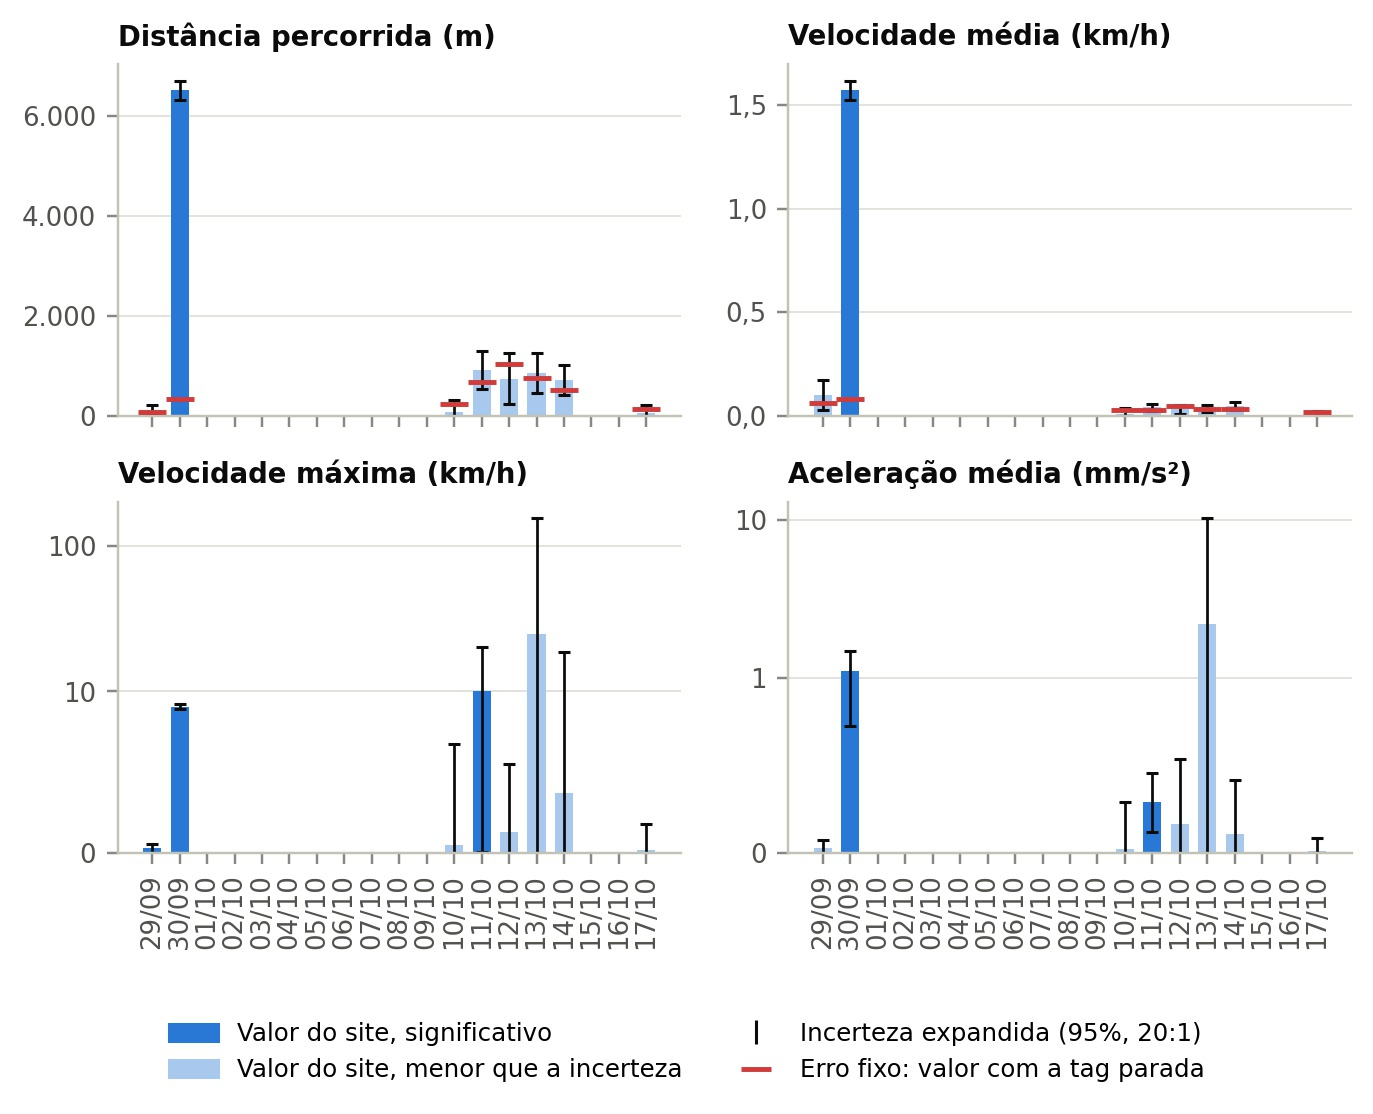
\includegraphics[width=\textwidth]{figuras/uc1_parametros.jpg}
  \fonte{Elaborado pelo autor (2026).}
\end{figure}

A Tabela~\ref{tab:uc1-dia30} reúne os resultados de 30/09, o dia com deslocamento, em 24 posições e 4 h 08 min. Todos os parâmetros foram significativos. A distância corrigida foi de $(6{,}19 \pm 0{,}19)$~km, com incerteza relativa de 3\%.

\begin{table}[htb]
  \centering
  \caption{Parâmetros de 30/09 a 95\% de confiança}
  \label{tab:uc1-dia30}
  \begin{tabular}{lrrr}
    \hline
    \textbf{Parâmetro} & \textbf{Valor do site} & \textbf{Erro fixo} & \textbf{Valor corrigido} \\
    \hline
    Distância percorrida & $(6{,}51 \pm 0{,}17)$ km & $(0{,}32 \pm 0{,}08)$ km & $(6{,}19 \pm 0{,}19)$ km \\
    Velocidade média & $(1{,}57 \pm 0{,}04)$ km/h & 0,08 km/h & $(1{,}50 \pm 0{,}05)$ km/h \\
    Velocidade máxima & $(9{,}0 \pm 0{,}2)$ km/h & --- & --- \\
    Aceleração média & $(1{,}1 \pm 0{,}4)$ mm/s² & --- & --- \\
    \hline
  \end{tabular}
  \fonte{Elaborado pelo autor (2026).}
\end{table}

Nos dias com a \textit{tag} parada, a distância corrigida foi compatível com zero. Em 11/10, por exemplo, o site somou 914 m, o erro fixo foi de 674 m e a distância corrigida, $(240 \pm 370)$~m. A velocidade máxima de 11/10, $(10 \pm 10)$~km/h, ficou no limite da significância, e a de 13/10, 24,7 km/h, teve incerteza de 130 km/h, porque vem de duas posições recebidas com poucos segundos de diferença. A Tabela~\ref{tab:uc1-total} reúne os parâmetros do intervalo total.

\begin{table}[htb]
  \centering
  \caption{Parâmetros calculados pelo site no intervalo total (29/09 a 17/10), a 95\% de confiança}
  \label{tab:uc1-total}
  \begin{tabular}{lrrr}
    \hline
    \textbf{Parâmetro} & \textbf{Valor do site} & \textbf{Erro fixo} & \textbf{Valor corrigido} \\
    \hline
    Distância percorrida & $(10{,}1 \pm 0{,}8)$ km & $(3{,}8 \pm 0{,}9)$ km & $(6{,}2 \pm 1{,}2)$ km \\
    Velocidade média & $(0{,}024 \pm 0{,}002)$ km/h & 0,009 km/h & $(0{,}015 \pm 0{,}003)$ km/h \\
    Velocidade máxima & $(25 \pm 130)$ km/h & --- & --- \\
    Aceleração média & $(0{,}7 \pm 1{,}7)$ mm/s² & --- & --- \\
    \hline
  \end{tabular}
  \fonte{Elaborado pelo autor (2026).}
\end{table}

A distância corrigida do intervalo total, $(6{,}2 \pm 1{,}2)$~km, coincide com a de 30/09: o restante dos 10,1 km somados pelo site corresponde ao ruído da posição nos dias parados. Um passo de comprimento próximo de zero tem incerteza de $\sqrt{2}\,\delta y = 39{,}5$~m, e 243 dos 274 passos do intervalo ficaram abaixo desse valor. A velocidade máxima e a aceleração média do intervalo total têm incerteza maior que o próprio valor e não permitem conclusões.

Com intervalos medianos de 16 min e incerteza de 19 m (leste) e 28 m (norte) a 95\% de confiança, a localização pela rede Find Hub atende à verificação da cerca virtual, sem posições na zona de dúvida. Para medir distância e velocidade em treinos, o cálculo do site precisaria descontar o erro fixo ou descartar passos menores que a incerteza de um passo, ou essas grandezas teriam de vir do acelerômetro.


% ---------------------------------------------------------------------
\section{Caso de uso 2: coleta biométrica}
\label{sec:res-biometria}

A Figura~\ref{fig:uc2-cobertura} mostra, para cada dia com o sensor ligado, quantos minutos têm leitura de cada sinal no servidor. O movimento somou 959 min e a temperatura 785 min. As leituras de frequência cardíaca somaram 304 s, distribuídos em oito janelas.

\begin{figure}[htb]
  \centering
  \caption{Minutos com leitura no servidor, por dia e por sinal}
  \label{fig:uc2-cobertura}
  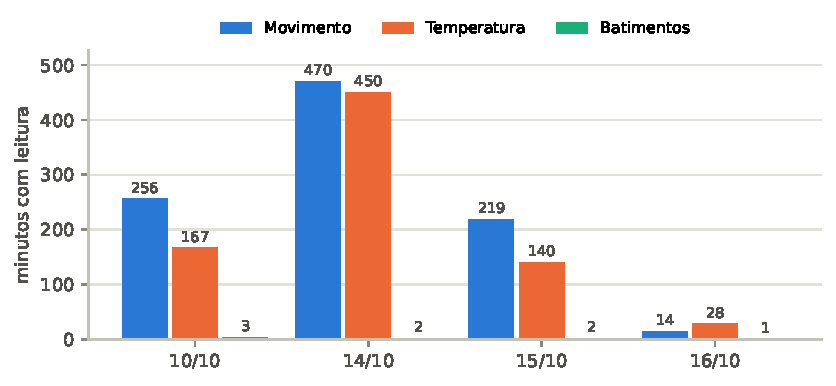
\includegraphics[width=0.95\linewidth]{figures/uc2_cobertura.pdf}
  \fonte{Elaborado pelo autor (2026).}
\end{figure}

A incerteza de cada sinal seguiu o mesmo procedimento do caso de uso 1 \cite{moffat1988}. A ordem zero é a metade da resolução do valor recebido \cite{poiate}; a primeira ordem é $2S$, com $S$ medido em um experimento auxiliar com o sensor em condição estável; o erro fixo vem da folha de dados ou de uma medição com valor conhecido; e a ordem $N$ é a soma quadrática dessas parcelas, a 95\% de confiança. A Tabela~\ref{tab:uc2-incerteza} resume os valores.

\begin{table}[htb]
  \centering
  \caption{Incerteza dos sinais biométricos a 95\% de confiança}
  \label{tab:uc2-incerteza}
  \begin{tabular}{lrrrr}
    \hline
    \textbf{Sinal} & \textbf{Ordem zero} & \textbf{1.ª ordem} & \textbf{Erro fixo} & \textbf{Ordem $N$} \\
    \hline
    Temperatura & 0,05 °C & 0,6 °C & 2,0 °C & 2,1 °C \\
    Movimento (minuto) & 0,00003 $g$ & 0,003 $g$ & 0,076 $g$ & 0,003 $g$\textsuperscript{a} \\
    Um batimento & 3,5 bpm & 6,0 bpm & não avaliado & 6,0 bpm \\
    Média de 16/10 & --- & 0,7 bpm & não avaliado & 0,7 bpm \\
    \hline
  \end{tabular}
  \fonte{Elaborado pelo autor (2026). \textsuperscript{a}Após descontar o erro fixo.}
\end{table}

\subsection{Frequência cardíaca}

O MAX30102 só calcula batimentos com pele encostada no sensor, e nos ensaios ele foi usado com o dedo do autor por poucos segundos. % CONFERIR
A Tabela~\ref{tab:bpm} lista as oito janelas. O sensor lê 25 vezes por segundo, e o intervalo entre dois picos tem resolução de 1/25 s. Pela propagação de $f = 60/T$, uma resolução $\delta T$ no período gera $\delta f = 60\,\delta T/T^2$ na frequência \cite{poiate}, valor que cresce com o quadrado da frequência: 3,5 bpm a 72 bpm e 21 bpm a 177 bpm.
% PROVISÓRIO: a janela de 16/10 00:03 tem valores fictícios (uc2.py, JANELA_PROVISORIA). Substituir pela medição real antes da entrega.

\begin{table}[htb]
  \centering
  \caption{Janelas com leitura de frequência cardíaca (bpm)}
  \label{tab:bpm}
  \begin{tabular}{lrrrrr}
    \hline
    \textbf{Início} & \textbf{Duração (s)} & \textbf{Média} & \textbf{Mínimo} & \textbf{Máximo} & \textbf{Resolução} \\
    \hline
    10/10 19:27 & 31 & 60,2 & 28,1 & 106,8 & 2,4 \\
    10/10 19:27 & 9 & 51,0 & 27,1 & 76,3 & 1,7 \\
    10/10 19:28 & 57 & 62,4 & 34,1 & 79,7 & 2,6 \\
    14/10 18:07 & 29 & 62,7 & 23,0 & 75,7 & 2,6 \\
    14/10 21:12 & 55 & 53,6 & 21,7 & 105,3 & 1,9 \\
    15/10 20:34 & 8 & 78,5 & 34,2 & 177,0 & 4,1 \\
    15/10 23:54 & 55 & 67,0 & 31,0 & 176,5 & 3,0 \\
    16/10 00:03 & 60 & 72,5 & 68,2 & 78,9 & 3,5 \\ % PROVISÓRIO
    \hline
  \end{tabular}
  \fonte{Elaborado pelo autor (2026). Resolução de um batimento na frequência média da janela.}
\end{table}

Nas sete primeiras janelas, os mínimos (22 a 34 bpm) e os máximos (até 177 bpm) se afastam da média muito mais que a resolução, o que mostra que o algoritmo de detecção de pulso aceitou picos falsos quando o dedo se moveu. O sensor dividia o barramento I2C com o MPU6050 em fios sem solda, e as falhas de contato desligaram a leitura de batimentos em parte do período. Na janela de 16/10, com 60 s de contato contínuo, a Figura~\ref{fig:uc2-batimentos} mostra os 73 batimentos. A média foi de $(72{,}5 \pm 0{,}7)$~bpm, com $S = 3{,}0$~bpm e $t = 1{,}99$ para 72 graus de liberdade, e a incerteza de um batimento isolado foi de $\pm 6{,}0$~bpm. Os valores se repetem em 68,2, 71,4, 75,0 e 78,9 bpm porque o período é contado em passos de 40 ms, e a resolução responde por boa parte da dispersão. O erro fixo do sensor exige comparação com um oxímetro de referência e não foi avaliado. % CONFERIR

\begin{figure}[htb]
  \centering
  \caption{Frequência de cada batimento na janela de 16/10, com a incerteza da média e de um batimento}
  \label{fig:uc2-batimentos}
  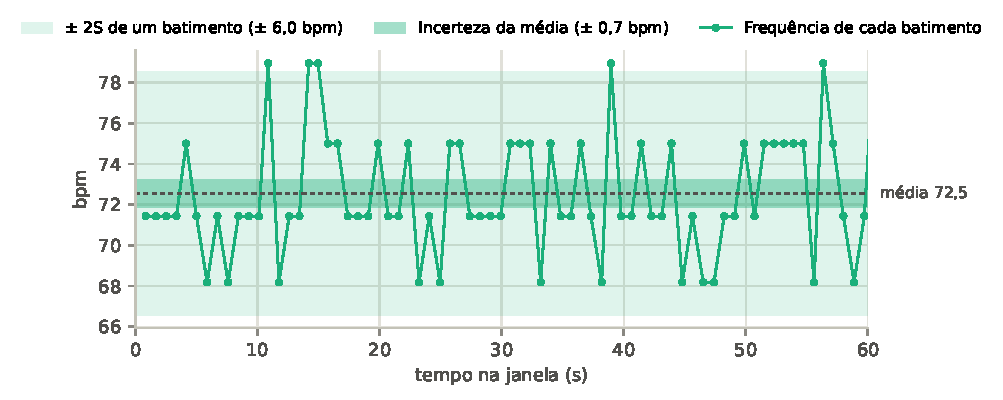
\includegraphics[width=0.95\linewidth]{figures/uc2_batimentos.pdf}
  \fonte{Elaborado pelo autor (2026).}
\end{figure}

\subsection{Temperatura}

A Figura~\ref{fig:uc2-temperatura} apresenta a temperatura como o portal a exibe, com a faixa de incerteza e os limites de alerta (35~°C e 40~°C) em vermelho. No dia 14/10 o DHT11 mediu o ar da sala, entre 24,0~°C e 27,9~°C em 450 leituras. A primeira ordem foi obtida das diferenças entre leituras sucessivas desse dia, que retiram a variação lenta da sala: $S = 0{,}30$~°C. A folha de dados do DHT11 informa exatidão de $\pm 2$~°C, adotada como erro fixo a 95\%. A ordem $N$ ficou em 2,1~°C, dominada pelo erro fixo.

\begin{figure}[htb]
  \centering
  \caption{Temperatura medida, incerteza e limites de alerta com as zonas de dúvida}
  \label{fig:uc2-temperatura}
  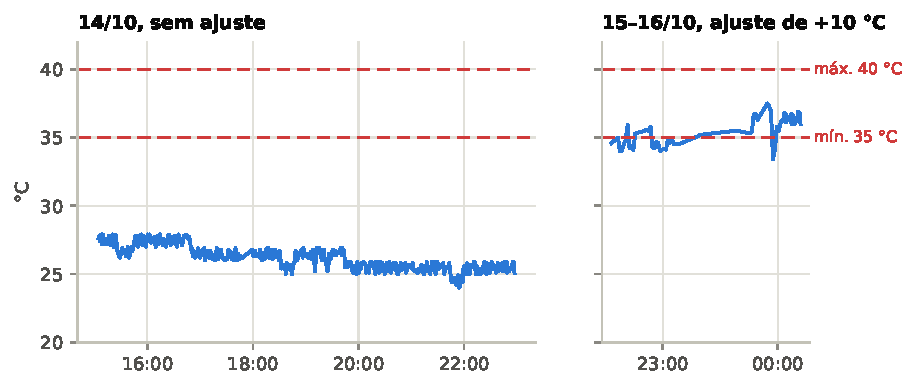
\includegraphics[width=0.95\linewidth]{figures/uc2_temperatura.pdf}
  \fonte{Elaborado pelo autor (2026).}
\end{figure}

Os limites de alerta formam uma tolerância de 5~°C. Pelo critério de \citeonline{poiate}, a incerteza deveria ficar abaixo de um décimo desse intervalo, 0,5~°C, e a do DHT11 é quatro vezes maior. A zona de aceitação fica reduzida a 37,1~°C a 37,9~°C, e as faixas de 32,9~°C a 37,1~°C e de 37,9~°C a 42,1~°C são zonas de dúvida, em que a medição não permite afirmar se a temperatura está dentro ou fora dos limites. As 450 leituras de 14/10 ficaram na zona de rejeição, abaixo do mínimo. Na noite de 15/10 foi salvo no portal um ajuste de +10~°C, usado para testar o caminho da calibração e não como correção medida. % CONFERIR
O sensor baixou o ajuste no envio seguinte e, a partir das 23h, as leituras passaram para a faixa de 33,4~°C a 37,5~°C: 47 das 49 leituras caíram na zona de dúvida e duas na zona de aceitação.

O teste confirma que o ajuste feito no portal chega ao sensor sem regravar o \textit{firmware} e passa a valer na comparação com os limites. O valor de +10~°C, porém, não corresponde a nenhuma referência e não reduz a incerteza: para uso no animal, o ajuste deve ser obtido comparando o sensor com um termômetro clínico, e um sensor com exatidão de 0,5~°C ou melhor atenderia ao critério de um décimo da tolerância.

\subsection{Movimento}

A Figura~\ref{fig:uc2-movimento} mostra a intensidade do movimento em 14/10, calculada como o afastamento do módulo da aceleração em relação a 1~$g$. Não havia limite de movimento configurado nesse dia. Nos 348 minutos com o sensor parado, a média por minuto foi de $(0{,}0761 \pm 0{,}0002)$~$g$, quando o esperado seria zero, com $S = 0{,}0016$~$g$ entre minutos. Nos 60 s mais estáveis das leituras brutas de 15/10, a 50 leituras/s, o módulo médio foi de 1,077~$g$, com $S = 0{,}003$~$g$ por leitura. O desvio de 0,076~$g$ é um erro fixo de escala do MPU6050, de 7,7\%, e é o motivo de o portal oferecer o ganho de calibração do movimento: com o ganho de $1/1{,}077$, a incerteza restante por minuto cai para 0,003~$g$. Sem a correção, o erro fixo precisa entrar na incerteza \cite{moffat1988}, e valores abaixo de cerca de 0,08~$g$ não se distinguem do sensor parado. Os picos de até 2,36~$g$ correspondem aos momentos em que o sensor foi manuseado e superam essa faixa com folga.

\begin{figure}[htb]
  \centering
  \caption{Intensidade do movimento por minuto em 14/10, com o erro fixo medido com o sensor parado (escala logarítmica acima de 0,1~$g$)}
  \label{fig:uc2-movimento}
  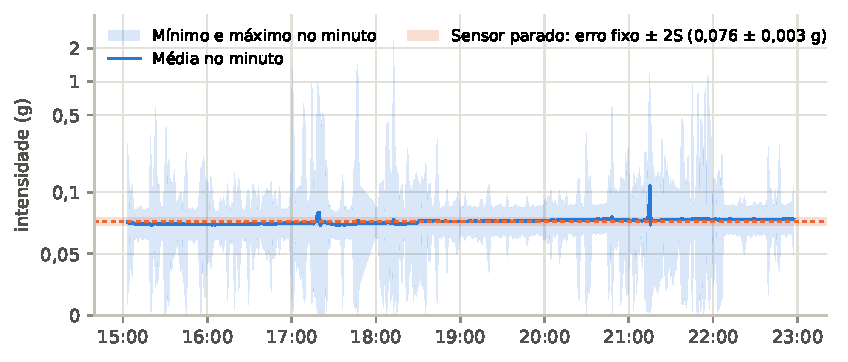
\includegraphics[width=0.95\linewidth]{figures/uc2_movimento.pdf}
  \fonte{Elaborado pelo autor (2026).}
\end{figure}

O envio de alertas por e-mail ao veterinário não foi avaliado, pois o servidor de e-mail (SMTP) não estava configurado no período. Os alertas pelo LED do sensor e pelo sino do portal foram verificados de forma visual, sem registro quantitativo. % CONFERIR

% ---------------------------------------------------------------------
\section{Caso de uso 3: detecção de padrões repetitivos}
\label{sec:res-padroes}

Os padrões ``Pulo'' e ``Volta'' foram avaliados em uma sessão de testes em 15/10, com 87,7 min de leituras do acelerômetro (263.089 amostras a 50 Hz). Nessa sessão o autor marcou no portal dez trechos, oito de Pulo e dois de Volta, que somam 22 s. Duas versões de detecção rodaram no sensor: até as 23h05, o modelo supervisionado treinado no servidor (floresta de 15 árvores de profundidade 4); depois desse horário, o detector físico descrito na metodologia.

A Figura~\ref{fig:uc3-sinal} mostra um trecho de 35 s com os três eixos, a marcação feita no portal (faixa cinza) e os eventos que o sensor registrou com o modelo supervisionado (linhas tracejadas).

\begin{figure}[htb]
  \centering
  \caption{Sinal do acelerômetro, trecho marcado como Pulo e eventos registrados pelo sensor}
  \label{fig:uc3-sinal}
  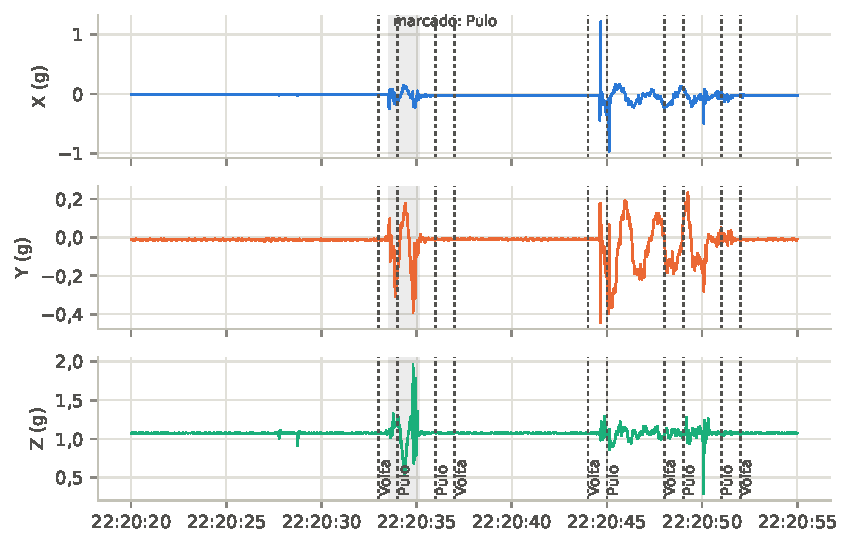
\includegraphics[width=0.95\linewidth]{figures/uc3_sinal_marcacoes.pdf}
  \fonte{Elaborado pelo autor (2026).}
\end{figure}

No trecho marcado, o eixo Z cai até cerca de 0,6~$g$ e sobe a quase 2~$g$, e o sensor registrou um Pulo dentro da marcação. O modelo, porém, também registrou eventos de Volta no mesmo instante e Pulos durante o manuseio seguinte, que não foi marcado. A Figura~\ref{fig:uc3-modelo} apresenta o desempenho do modelo supervisionado na validação feita pelo servidor no treino, deixando uma marcação de fora de cada vez.

\begin{figure}[htb]
  \centering
  \caption{Desempenho do modelo supervisionado na validação do treino}
  \label{fig:uc3-modelo}
  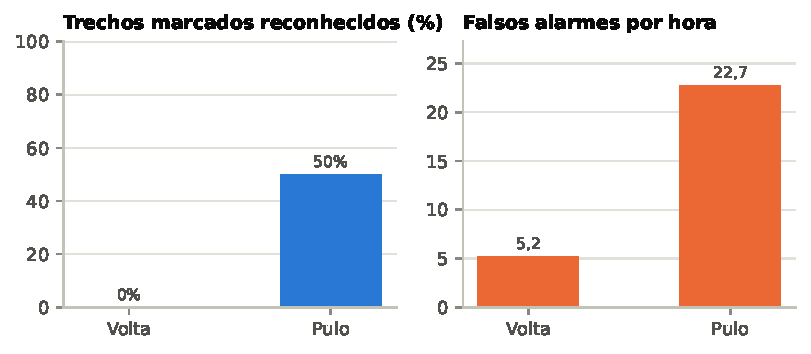
\includegraphics[width=0.95\linewidth]{figures/uc3_modelo_supervisionado.pdf}
  \fonte{Elaborado pelo autor (2026).}
\end{figure}

O modelo reconheceu 50\% dos trechos de Pulo, com 22,7 falsos alarmes por hora fora das marcações, e nenhum trecho de Volta. Com oito exemplos de Pulo (31 janelas) contra 3.000 janelas negativas, e dois exemplos de Volta, a base de treino é pequena demais para separar os padrões do manuseio comum do sensor. Esse resultado levou à troca do modelo supervisionado por um detector baseado na física do movimento, que não depende de exemplos marcados.

No detector físico, um salto é identificado pelo tempo $T$ em queda livre, em que o módulo da aceleração fica abaixo de 0,6~$g$. A altura vem da equação do lançamento vertical, $h = gT^2/8$, e o salto só é contado acima de 5~cm. A Figura~\ref{fig:uc3-voo} mostra os 20 voos com pelo menos 0,06 s encontrados ao reaplicar essa regra às leituras da sessão.

\begin{figure}[htb]
  \centering
  \caption{Altura estimada de cada voo pelo tempo em queda livre e limiar de contagem}
  \label{fig:uc3-voo}
  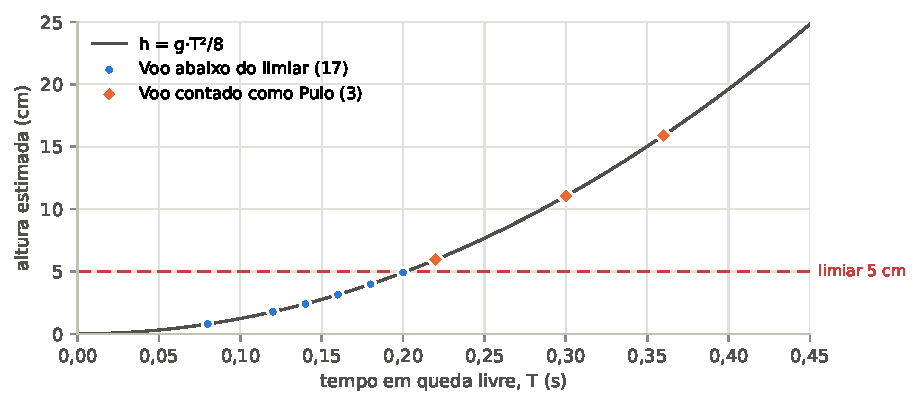
\includegraphics[width=0.95\linewidth]{figures/uc3_voo_altura.pdf}
  \fonte{Elaborado pelo autor (2026).}
\end{figure}

Três voos passaram do limiar, com 5,9 cm, 11 cm e 15,9 cm; os outros 17 ficaram entre 0,8 cm e 4,9 cm. Os oito trechos marcados como Pulo tiveram voos abaixo de 5 cm, de modo que nenhum deles foi contado. Os saltos do teste foram pequenos, feitos levantando e soltando a placa, e ficaram na faixa em que a regra não distingue um salto de um solavanco. Em um cavalo, um salto de 1 m corresponde a cerca de 0,9 s em queda livre, valor muito acima do ruído observado.

A Tabela~\ref{tab:uc3} compara as duas versões. A versão supervisionada é a que rodou no sensor até as 23h05; a física foi reaplicada às leituras da sessão inteira. Os eventos fora das marcações não equivalem a falsos alarmes, pois o autor não marcou todos os movimentos feitos durante a sessão.

\begin{table}[htb]
  \centering
  \caption{Marcações reconhecidas e eventos por versão de detecção na sessão de 15/10}
  \label{tab:uc3}
  \begin{tabular}{llrrr}
    \hline
    \textbf{Padrão} & \textbf{Versão} & \textbf{Marcações} & \textbf{Reconhecidas} & \textbf{Eventos} \\
    \hline
    Pulo  & Supervisionada (sensor) & 6 & 1 & 39 \\
    Volta & Supervisionada (sensor) & 2 & 0 & 42 \\
    Pulo  & Física (reaplicada) & 8 & 0 & 3 \\
    Volta & Física (reaplicada) & 2 & 2 & 22 \\
    \hline
  \end{tabular}
  \fonte{Elaborado pelo autor (2026).}
\end{table}

Para a Volta, o detector físico reconheceu os dois trechos marcados ao somar 360° de rotação do vetor horizontal da aceleração, e registrou 22 voltas na sessão, contra 42 do modelo supervisionado em um período menor. A reaplicação usou apenas o método do vetor horizontal, pois as leituras do giroscópio não ficam guardadas no servidor; no sensor, a volta também é contada pela rotação medida pelo giroscópio.

% ---------------------------------------------------------------------
\section{Caso de uso 4}
\label{sec:res-uc4}

% PENDENTE: resultados do caso de uso 4.
Os resultados deste caso de uso serão apresentados após a conclusão dos ensaios.

% ---------------------------------------------------------------------
\section{Síntese dos resultados}
\label{sec:res-sintese}

O protótipo coletou e enviou ao servidor 959 min de movimento e 785 min de temperatura em quatro dias, com as leituras guardadas no cartão SD entre um envio e outro. A localização pela rede Find Hub detectou a saída da cerca em 30/09, com posições a cada 16 min (mediana) e incerteza de 19 m (leste) e 28 m (norte) a 95\% de confiança. Com essa incerteza, o site soma cerca de 14 m por passo com a \textit{tag} parada, e a distância só foi significativa no dia com deslocamento. A calibração e os limites definidos no portal chegaram ao sensor sem regravar o \textit{firmware}. A frequência cardíaca teve 304 s de leitura, limitada pelo contato com a pele e pelas conexões do barramento I2C, e a janela com contato contínuo deu $(72{,}5 \pm 0{,}7)$~bpm. % PROVISÓRIO: valor da janela fictícia de 16/10
A temperatura teve incerteza de 2,1~°C, quatro vezes o recomendado para os limites de alerta, e o movimento, um erro fixo de 0,076~$g$ que o ganho de calibração corrige. Na detecção de padrões, o modelo supervisionado não atingiu desempenho útil com dez marcações, e o detector físico reconheceu as voltas marcadas, mas os saltos de teste ficaram abaixo do limiar de 5 cm. Os ensaios no animal são a próxima etapa para medir esses valores em condições reais.
. As figuras estão em figures/ (PDF vetorial; o PNG
% de mesmo nome serve para visualização).
%
% Estrutura (NBR 14724): o capítulo abre com as condições dos ensaios,
% segue a ordem dos casos de uso definidos na metodologia, cita cada
% figura e tabela no texto antes de ela aparecer, traz o título acima e a
% fonte abaixo, e discute cada resultado logo depois de apresentá-lo.
%
% Trechos marcados com "CONFERIR" dependem de informação que só o autor
% tem (condições dos ensaios). Revise antes de entregar.
%
% PROVISÓRIO: a janela de batimentos de 16/10 00:03 (caso de uso 2) tem
% valores fictícios. Substituir pela medição real antes da entrega.
% =====================================================================

\chapter{Resultados e discussão}
\label{cap:resultados}

Este capítulo apresenta os resultados obtidos com o protótipo entre 29 de setembro e 17 de outubro de 2026, organizados pelos casos de uso definidos na metodologia: localização (caso de uso 1), coleta biométrica (caso de uso 2), detecção de padrões repetitivos de movimento (caso de uso 3) e o caso de uso 4, ainda em andamento. Os dados foram extraídos da API do portal, a mesma que alimenta as telas do sistema, e processados por \textit{scripts} em Python para gerar as figuras.

Os ensaios foram feitos com o protótipo fora do animal: o sensor ficou sobre a bancada na maior parte do tempo e foi movimentado à mão nos testes de padrões, e a \textit{tag} de localização permaneceu em área urbana. % CONFERIR: condições dos ensaios
A Tabela~\ref{tab:condicoes} resume a configuração usada.

\begin{table}[htb]
  \centering
  \caption{Configuração do protótipo durante os ensaios}
  \label{tab:condicoes}
  \begin{tabular}{lp{8.5cm}}
    \hline
    \textbf{Item} & \textbf{Valor} \\
    \hline
    Microcontrolador & ESP32 DevKit \\
    Acelerômetro e giroscópio & MPU6050, 50 leituras/s \\
    Frequência cardíaca & MAX30102, 25 leituras/s \\
    Temperatura & DHT11, uma leitura a cada 20 s \\
    Armazenamento local & cartão microSD \\
    Intervalo de envio ao servidor & 180 s \\
    Localização & \textit{tag} BLE na rede Google Find Hub, consulta a cada 10 min \\
    Cerca virtual & círculo de 310 m de raio \\
    Período analisado & localização: 29/09 a 17/10/2026; sensor: 10/10 a 16/10/2026 \\
    \hline
  \end{tabular}
  \fonte{Elaborado pelo autor (2026).}
\end{table}

% ---------------------------------------------------------------------
% =====================================================================
% Caso de uso 1 (localização). Seção do capítulo de resultados, incluída
% em resultados.tex com % =====================================================================
% Caso de uso 1 (localização). Seção do capítulo de resultados, incluída
% em resultados.tex com \input{resultados_uc1}. Figuras em figuras/*.jpg.
% Incerteza: Moffat (1988) e Poiate Junior (apostila), chaves em referencias.bib.
% Trechos marcados com "CONFERIR" dependem de informação do autor.
% =====================================================================

\section{Caso de uso 1: localização}
\label{sec:res-localizacao}

O intervalo analisado vai de 29/09/2026 a 17/10/2026 e reúne 275 posições da \textit{tag}. As 32 primeiras, até 10/10, foram coletadas pela instância local do servidor, antes da implantação; as 243 seguintes, pela instância em produção. As duas instâncias usam o mesmo código de consulta e de filtragem. Entre 30/09 e 10/10 não há posições, porque o servidor local ficou desligado nesse período. % CONFERIR: motivo da lacuna
As posições estão em metros a partir do centro da cerca virtual, sem mapa de fundo, para não expor o endereço do local de teste.

A Figura~\ref{fig:uc1-trajeto} apresenta as posições em duas escalas. Em (a), o período de 10/10 a 17/10, com a \textit{tag} parada dentro da cerca de 310 m de raio. Em (b), o intervalo total, que inclui o deslocamento a pé feito pelo autor em 30/09.

\begin{figure}[htb]
  \centering
  \caption{Posições recebidas da \textit{tag} e cerca virtual: (a) período com a \textit{tag} parada; (b) intervalo total}
  \label{fig:uc1-trajeto}
  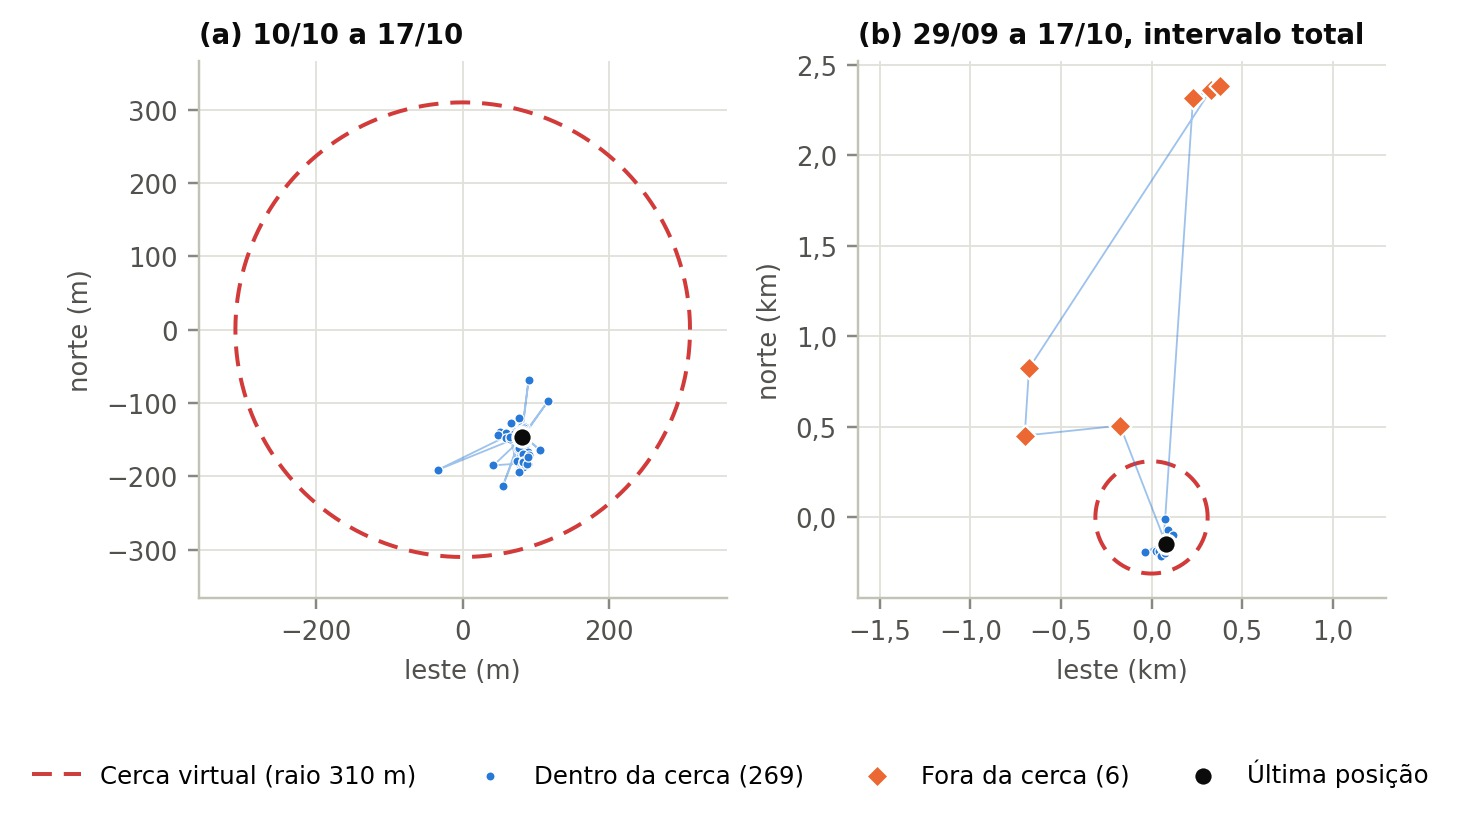
\includegraphics[width=\textwidth]{figuras/uc1_trajeto.jpg}
  \fonte{Elaborado pelo autor (2026).}
\end{figure}

Seis posições ficaram fora da cerca, todas em 30/09, entre 13h32 e 14h31, a até 2,41 km do centro. O site registrou o alerta de saída da cerca a partir da primeira delas: o cartão de localização do cavalo passou a indicar ``Fora da cerca'' e o alerta apareceu no sino do portal. Nas demais 269 posições a \textit{tag} estava dentro do raio.

A Figura~\ref{fig:uc1-dia} mostra quantas posições chegaram em cada dia. A quantidade variou de 6 a 75 por dia. A rede Find Hub depende de celulares Android que passem perto da \textit{tag}, e o servidor só registra o que a rede entrega.

\begin{figure}[htb]
  \centering
  \caption{Posições recebidas por dia, dentro e fora da cerca}
  \label{fig:uc1-dia}
  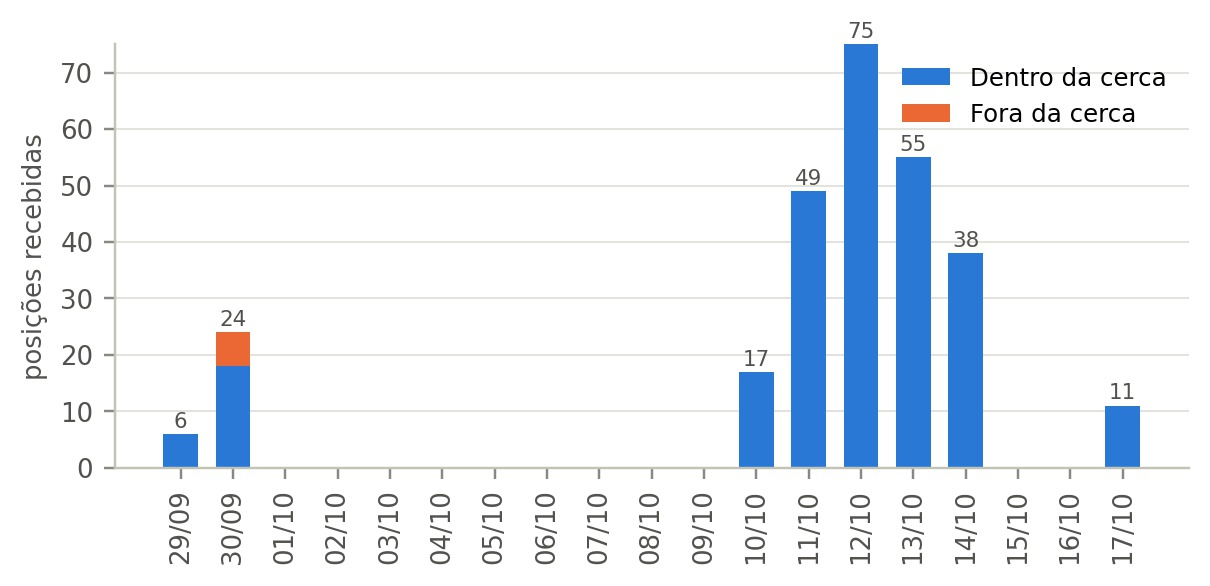
\includegraphics[width=\textwidth]{figuras/uc1_por_dia.jpg}
  \fonte{Elaborado pelo autor (2026).}
\end{figure}

A Figura~\ref{fig:uc1-intervalo} apresenta o intervalo entre posições consecutivas e a precisão informada pela rede em cada posição. O intervalo mediano foi de 16 min, e 90\% dos intervalos ficaram abaixo de 57 min; o maior intervalo, de 239 h, corresponde à lacuna entre 30/09 e 10/10. A precisão informada teve mediana de 75 m, e 46\% das posições chegaram com o valor máximo aceito pelo filtro do servidor, 100 m.

\begin{figure}[htb]
  \centering
  \caption{Intervalo entre posições consecutivas e precisão informada pela rede}
  \label{fig:uc1-intervalo}
  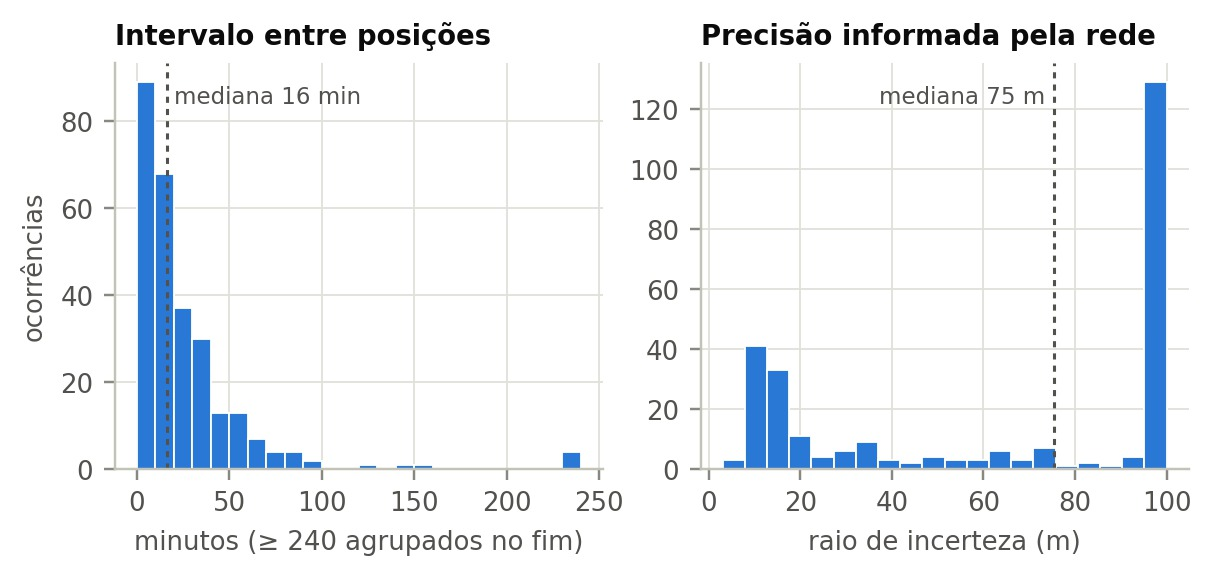
\includegraphics[width=\textwidth]{figuras/uc1_intervalo_precisao.jpg}
  \fonte{Elaborado pelo autor (2026).}
\end{figure}

\subsection{Incerteza da posição}
\label{sec:uc1-incerteza-posicao}

A incerteza foi avaliada pela análise de amostra única de \citeonline{moffat1988}: cada posição é uma leitura isolada, e a dispersão do sistema de medição é obtida de um experimento auxiliar feito em condição representativa. O experimento auxiliar foi o período de 10/10 a 17/10, com a \textit{tag} parada no mesmo ponto e 243 leituras. As coordenadas foram convertidas para metros nas direções leste ($x$) e norte ($y$), e o desvio-padrão amostral de cada direção foi $S_x = 9{,}6$~m e $S_y = 14{,}0$~m.

Com 242 graus de liberdade, a distribuição qui-quadrado limita o desvio-padrão da população a $0{,}92\,S \le \sigma \le 1{,}10\,S$, ao nível de 95\% \cite{moffat1988}. Foi adotado o valor mais provável, $\sigma = S$. A incerteza de uma leitura isolada, a 95\% de confiança (chance de 20 para 1), é
\begin{equation}
  \delta x = 2\sigma_x = 19{,}2~\text{m}, \qquad \delta y = 2\sigma_y = 27{,}9~\text{m}.
  \label{eq:uc1-incerteza-posicao}
\end{equation}
Com o limite superior de $\sigma$, os valores seriam 21,0 m e 30,6 m. Nos dados, 96,3\% das leituras ficaram dentro de $\pm\delta x$ e 92,2\% dentro de $\pm\delta y$. A distribuição não é gaussiana, pois 92\% das leituras na direção leste ficaram dentro de $\pm S_x$, e uma leitura isolada se afastou 121 m da média. A autocorrelação entre leituras consecutivas foi de $-0{,}001$ (leste) e $0{,}12$ (norte), e as leituras foram tratadas como independentes, condição exigida para a soma quadrática.

A Tabela~\ref{tab:uc1-ordens} separa a incerteza da posição nas três ordens de \citeonline{moffat1988}. A ordem zero corresponde à resolução dos valores recebidos, que chegam com $10^{-7}$ grau (cerca de 1,1 cm), e a incerteza instrumental é a metade da resolução \cite{poiate}. O horário de cada posição chega em segundos inteiros, com incerteza de 0,5 s. A primeira ordem é a dispersão medida no experimento auxiliar. Na ordem $N$ entraria o erro fixo da rede, isto é, a diferença entre a média das leituras e a posição verdadeira da \textit{tag}. Esse erro não foi medido, porque não havia uma referência de posição com incerteza menor; ele desloca todas as leituras da mesma forma, e por isso se cancela nas diferenças entre posições usadas na distância e na velocidade, mas afeta a verificação da cerca.

\begin{table}[htb]
  \centering
  \caption{Incerteza de uma posição a 95\% de confiança}
  \label{tab:uc1-ordens}
  \begin{tabular}{lrrl}
    \hline
    \textbf{Ordem} & \textbf{Leste (m)} & \textbf{Norte (m)} & \textbf{Origem} \\
    \hline
    Zero & 0,005 & 0,006 & resolução de $10^{-7}$ grau \\
    Primeira & 19,2 & 27,9 & experimento auxiliar, $2S$ \\
    $N$ & 19,2 & 27,9 & erro fixo da rede não avaliado \\
    \hline
  \end{tabular}
  \fonte{Elaborado pelo autor (2026).}
\end{table}

A ordem zero é cerca de 4 mil vezes menor que a primeira e foi desprezada, pois uma parcela menor que um terço da maior tem efeito pequeno na soma quadrática \cite{moffat1988}. Em 95,9\% das leituras paradas, a distância até a média ficou abaixo da precisão informada pela rede para aquela leitura, cuja mediana foi de 75 m. A precisão informada se comporta como um limite conservador, maior que a incerteza medida.

\subsection{Verificação da cerca com a incerteza}

A cerca virtual funciona como uma tolerância: a posição é aceita enquanto a distância $r$ até o centro não passa do raio $R = 310$~m. Seguindo \citeonline{poiate}, a incerteza de medição divide a faixa em três zonas. A zona de aceitação vai até $R - \delta r$, a zona de rejeição começa em $R + \delta r$ e, entre as duas, fica a zona de dúvida, onde a medição não permite afirmar se a \textit{tag} está dentro ou fora. A incerteza da distância ao centro vem da propagação das incertezas da Equação~\eqref{eq:uc1-incerteza-posicao}:
\begin{equation}
  \delta r = \sqrt{\left(\frac{x}{r}\,\delta x\right)^2 + \left(\frac{y}{r}\,\delta y\right)^2}.
  \label{eq:uc1-incerteza-raio}
\end{equation}

O maior valor de $\delta r$ entre as posições foi de 27,8 m, o que coloca a zona de dúvida entre 282 m e 338 m. A incerteza ficou abaixo de um décimo do intervalo de tolerância (31 m), critério de equilíbrio entre custo e qualidade recomendado por \citeonline{poiate}. A Figura~\ref{fig:uc1-zonas} mostra a distância de cada posição ao centro com as três zonas.

\begin{figure}[htb]
  \centering
  \caption{Distância das posições ao centro da cerca, com as zonas de aceitação, dúvida e rejeição}
  \label{fig:uc1-zonas}
  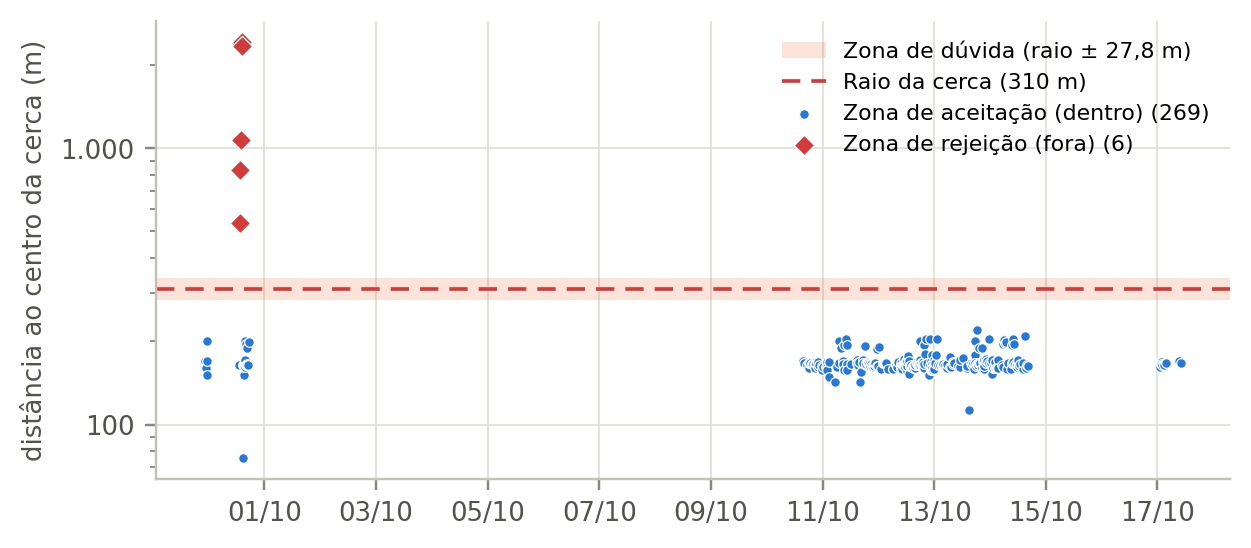
\includegraphics[width=\textwidth]{figuras/uc1_zonas.jpg}
  \fonte{Elaborado pelo autor (2026).}
\end{figure}

As 269 posições dentro da cerca ficaram a até 220 m do centro, na zona de aceitação. As seis posições de 30/09 ficaram a pelo menos 536 m, na zona de rejeição, e nenhuma posição caiu na zona de dúvida. O alerta de saída da cerca de 30/09 não depende, portanto, da incerteza da posição.

\subsection{Parâmetros calculados pelo site}

O site calcula, a partir das posições gravadas no banco, quatro parâmetros para o intervalo escolhido. A distância percorrida é a soma das distâncias entre posições consecutivas, $d = \sum_k s_k$. A velocidade média é essa distância dividida pelo tempo $T$ entre a primeira e a última posição. A velocidade máxima é a maior razão $s_k/\Delta t_k$ entre duas posições consecutivas. A aceleração média é a média das variações de velocidade entre trechos seguidos.

A incerteza desses resultados foi propagada pelo método da perturbação sequencial \cite{moffat1988}, aplicado à mesma função de cálculo do site. Cada entrada $X_i$ (latitude, longitude e horário de cada posição) foi aumentada e reduzida pela sua incerteza $\delta X_i$, uma de cada vez, e a contribuição $C_i$ foi tomada como a média de $|R_{i+} - R_0|$ e $|R_{i-} - R_0|$, porque o resultado não é linear nas posições. A incerteza do resultado é a soma quadrática das contribuições,
\begin{equation}
  \delta R = \sqrt{\sum_i C_i^2}, \qquad C_i \approx \frac{\partial R}{\partial X_i}\,\delta X_i,
  \label{eq:uc1-perturbacao}
\end{equation}
e tem o mesmo nível de confiança das entradas, 95\%. Para a velocidade média, a propagação analítica da apostila de \citeonline{poiate},
\begin{equation}
  \frac{\delta \bar v}{\bar v} = \sqrt{\left(\frac{\delta d}{d}\right)^2 + \left(\frac{\delta T}{T}\right)^2},
  \label{eq:uc1-vmed}
\end{equation}
com $\delta T = 1$~s (metade da resolução em cada extremo), deu o mesmo valor que a perturbação sequencial até a terceira casa. A parcela do horário foi desprezível em todos os resultados, exceto na velocidade máxima de 13/10, em que foi de 23 km/h contra 128 km/h da parcela das posições.

A soma de passos tem também um erro fixo, que \citeonline{moffat1988} classifica como erro conceitual: com a \textit{tag} parada, o ruído da posição gera passos de comprimento não nulo, e o site os soma como distância. Esse erro foi medido no experimento auxiliar, com 121 pares de leituras consecutivas sem leitura em comum. O passo médio foi de $(14{,}0 \pm 3{,}3)$~m, em que a incerteza é $t\,S/\sqrt{N}$, com $t = 1{,}98$ para 120 graus de liberdade. Para um intervalo com $k$ passos, o erro fixo é $B = k \times 14{,}0$~m, e a sua incerteza, $k \times 3{,}3$~m, somada de forma linear, porque o mesmo valor médio é usado em todos os passos. A distância corrigida é $d - B$, e a sua incerteza de ordem $N$ é a soma quadrática da incerteza propagada com a incerteza de $B$. Essa correção supõe a \textit{tag} parada em todos os passos e, nos dias com deslocamento, superestima o erro fixo. A velocidade média recebe a mesma correção, dividida por $T$.

A Figura~\ref{fig:uc1-parametros} apresenta, por dia, o valor calculado pelo site, a incerteza expandida e o erro fixo. Um valor foi considerado significativo quando superou a sua incerteza, isto é, quando a diferença em relação a zero (ou ao erro fixo, no caso da distância e da velocidade média) foi maior que a incerteza dessa diferença \cite{moffat1988}.

\begin{figure}[htb]
  \centering
  \caption{Parâmetros calculados pelo site por dia, com a incerteza expandida e o erro fixo}
  \label{fig:uc1-parametros}
  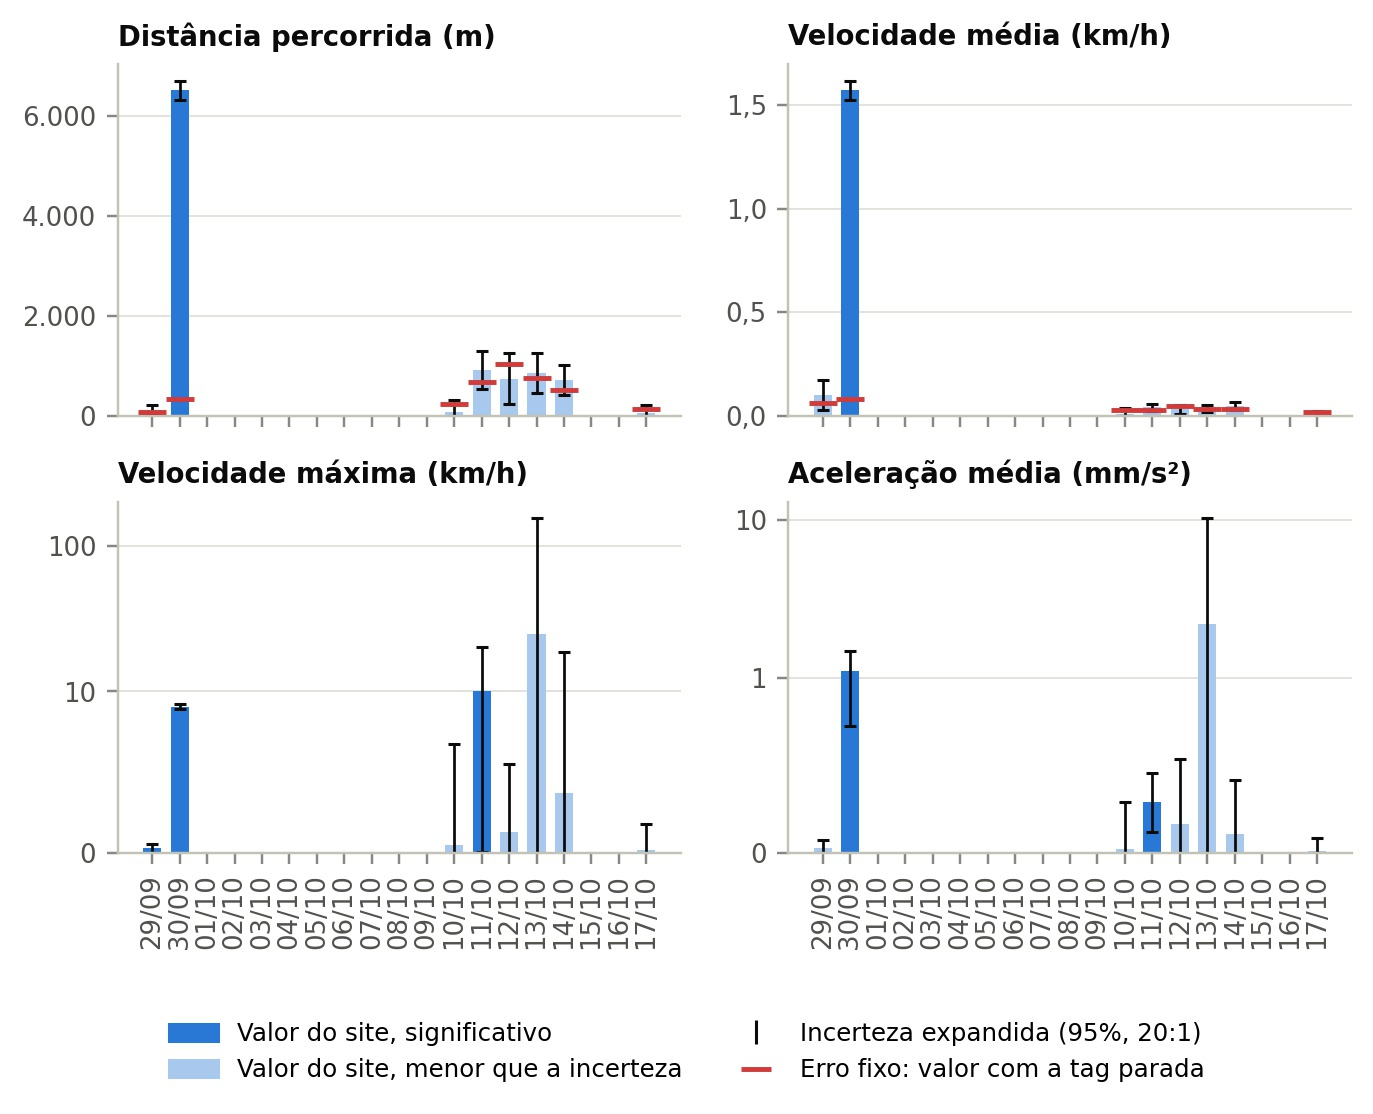
\includegraphics[width=\textwidth]{figuras/uc1_parametros.jpg}
  \fonte{Elaborado pelo autor (2026).}
\end{figure}

A Tabela~\ref{tab:uc1-dia30} reúne os resultados de 30/09, o dia com deslocamento, em 24 posições e 4 h 08 min. Todos os parâmetros foram significativos. A distância corrigida foi de $(6{,}19 \pm 0{,}19)$~km, com incerteza relativa de 3\%.

\begin{table}[htb]
  \centering
  \caption{Parâmetros de 30/09 a 95\% de confiança}
  \label{tab:uc1-dia30}
  \begin{tabular}{lrrr}
    \hline
    \textbf{Parâmetro} & \textbf{Valor do site} & \textbf{Erro fixo} & \textbf{Valor corrigido} \\
    \hline
    Distância percorrida & $(6{,}51 \pm 0{,}17)$ km & $(0{,}32 \pm 0{,}08)$ km & $(6{,}19 \pm 0{,}19)$ km \\
    Velocidade média & $(1{,}57 \pm 0{,}04)$ km/h & 0,08 km/h & $(1{,}50 \pm 0{,}05)$ km/h \\
    Velocidade máxima & $(9{,}0 \pm 0{,}2)$ km/h & --- & --- \\
    Aceleração média & $(1{,}1 \pm 0{,}4)$ mm/s² & --- & --- \\
    \hline
  \end{tabular}
  \fonte{Elaborado pelo autor (2026).}
\end{table}

Nos dias com a \textit{tag} parada, a distância corrigida foi compatível com zero. Em 11/10, por exemplo, o site somou 914 m, o erro fixo foi de 674 m e a distância corrigida, $(240 \pm 370)$~m. A velocidade máxima de 11/10, $(10 \pm 10)$~km/h, ficou no limite da significância, e a de 13/10, 24,7 km/h, teve incerteza de 130 km/h, porque vem de duas posições recebidas com poucos segundos de diferença. A Tabela~\ref{tab:uc1-total} reúne os parâmetros do intervalo total.

\begin{table}[htb]
  \centering
  \caption{Parâmetros calculados pelo site no intervalo total (29/09 a 17/10), a 95\% de confiança}
  \label{tab:uc1-total}
  \begin{tabular}{lrrr}
    \hline
    \textbf{Parâmetro} & \textbf{Valor do site} & \textbf{Erro fixo} & \textbf{Valor corrigido} \\
    \hline
    Distância percorrida & $(10{,}1 \pm 0{,}8)$ km & $(3{,}8 \pm 0{,}9)$ km & $(6{,}2 \pm 1{,}2)$ km \\
    Velocidade média & $(0{,}024 \pm 0{,}002)$ km/h & 0,009 km/h & $(0{,}015 \pm 0{,}003)$ km/h \\
    Velocidade máxima & $(25 \pm 130)$ km/h & --- & --- \\
    Aceleração média & $(0{,}7 \pm 1{,}7)$ mm/s² & --- & --- \\
    \hline
  \end{tabular}
  \fonte{Elaborado pelo autor (2026).}
\end{table}

A distância corrigida do intervalo total, $(6{,}2 \pm 1{,}2)$~km, coincide com a de 30/09: o restante dos 10,1 km somados pelo site corresponde ao ruído da posição nos dias parados. Um passo de comprimento próximo de zero tem incerteza de $\sqrt{2}\,\delta y = 39{,}5$~m, e 243 dos 274 passos do intervalo ficaram abaixo desse valor. A velocidade máxima e a aceleração média do intervalo total têm incerteza maior que o próprio valor e não permitem conclusões.

Com intervalos medianos de 16 min e incerteza de 19 m (leste) e 28 m (norte) a 95\% de confiança, a localização pela rede Find Hub atende à verificação da cerca virtual, sem posições na zona de dúvida. Para medir distância e velocidade em treinos, o cálculo do site precisaria descontar o erro fixo ou descartar passos menores que a incerteza de um passo, ou essas grandezas teriam de vir do acelerômetro.
. Figuras em figuras/*.jpg.
% Incerteza: Moffat (1988) e Poiate Junior (apostila), chaves em referencias.bib.
% Trechos marcados com "CONFERIR" dependem de informação do autor.
% =====================================================================

\section{Caso de uso 1: localização}
\label{sec:res-localizacao}

O intervalo analisado vai de 29/09/2026 a 17/10/2026 e reúne 275 posições da \textit{tag}. As 32 primeiras, até 10/10, foram coletadas pela instância local do servidor, antes da implantação; as 243 seguintes, pela instância em produção. As duas instâncias usam o mesmo código de consulta e de filtragem. Entre 30/09 e 10/10 não há posições, porque o servidor local ficou desligado nesse período. % CONFERIR: motivo da lacuna
As posições estão em metros a partir do centro da cerca virtual, sem mapa de fundo, para não expor o endereço do local de teste.

A Figura~\ref{fig:uc1-trajeto} apresenta as posições em duas escalas. Em (a), o período de 10/10 a 17/10, com a \textit{tag} parada dentro da cerca de 310 m de raio. Em (b), o intervalo total, que inclui o deslocamento a pé feito pelo autor em 30/09.

\begin{figure}[htb]
  \centering
  \caption{Posições recebidas da \textit{tag} e cerca virtual: (a) período com a \textit{tag} parada; (b) intervalo total}
  \label{fig:uc1-trajeto}
  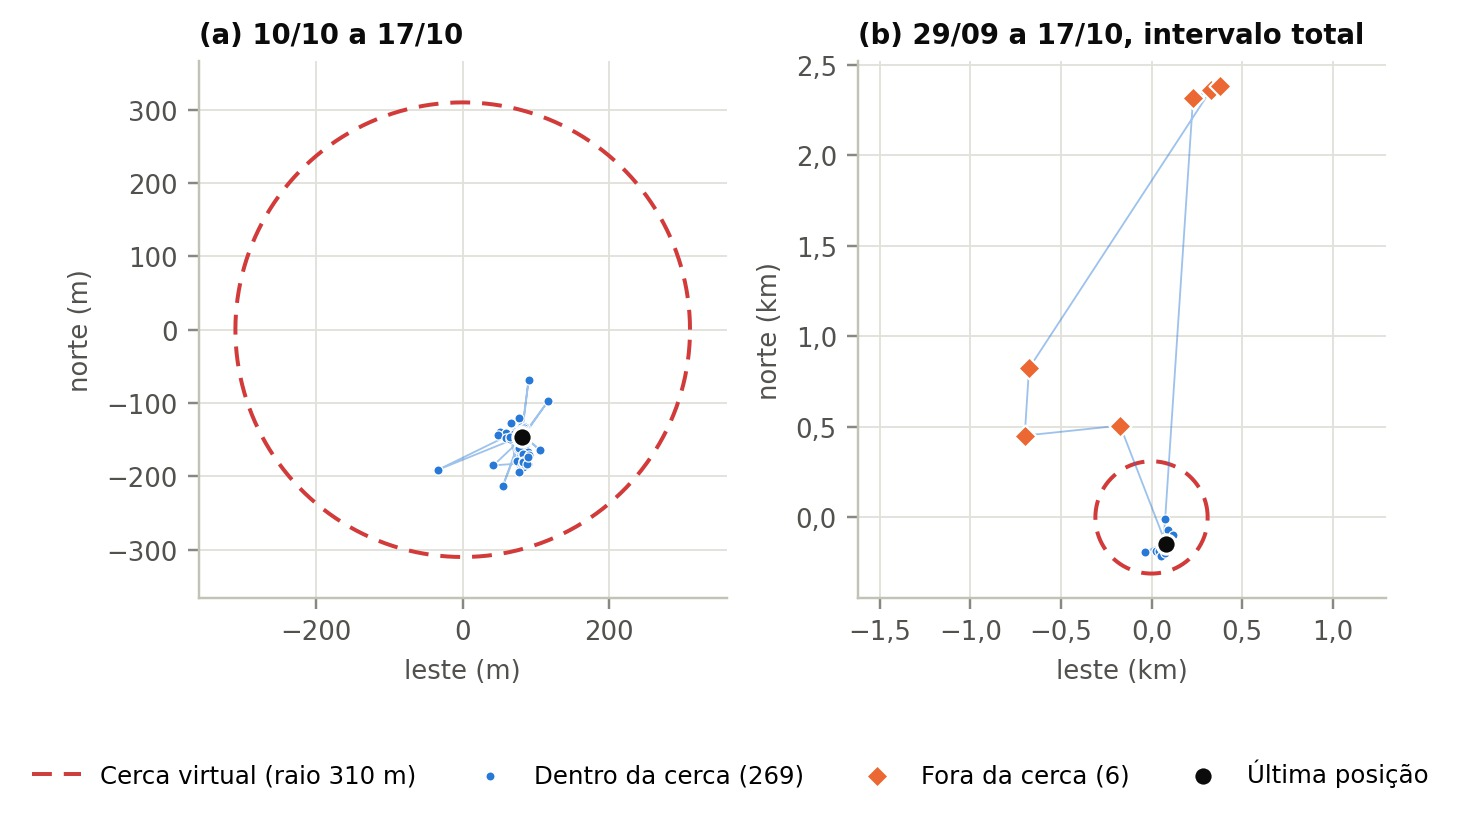
\includegraphics[width=\textwidth]{figuras/uc1_trajeto.jpg}
  \fonte{Elaborado pelo autor (2026).}
\end{figure}

Seis posições ficaram fora da cerca, todas em 30/09, entre 13h32 e 14h31, a até 2,41 km do centro. O site registrou o alerta de saída da cerca a partir da primeira delas: o cartão de localização do cavalo passou a indicar ``Fora da cerca'' e o alerta apareceu no sino do portal. Nas demais 269 posições a \textit{tag} estava dentro do raio.

A Figura~\ref{fig:uc1-dia} mostra quantas posições chegaram em cada dia. A quantidade variou de 6 a 75 por dia. A rede Find Hub depende de celulares Android que passem perto da \textit{tag}, e o servidor só registra o que a rede entrega.

\begin{figure}[htb]
  \centering
  \caption{Posições recebidas por dia, dentro e fora da cerca}
  \label{fig:uc1-dia}
  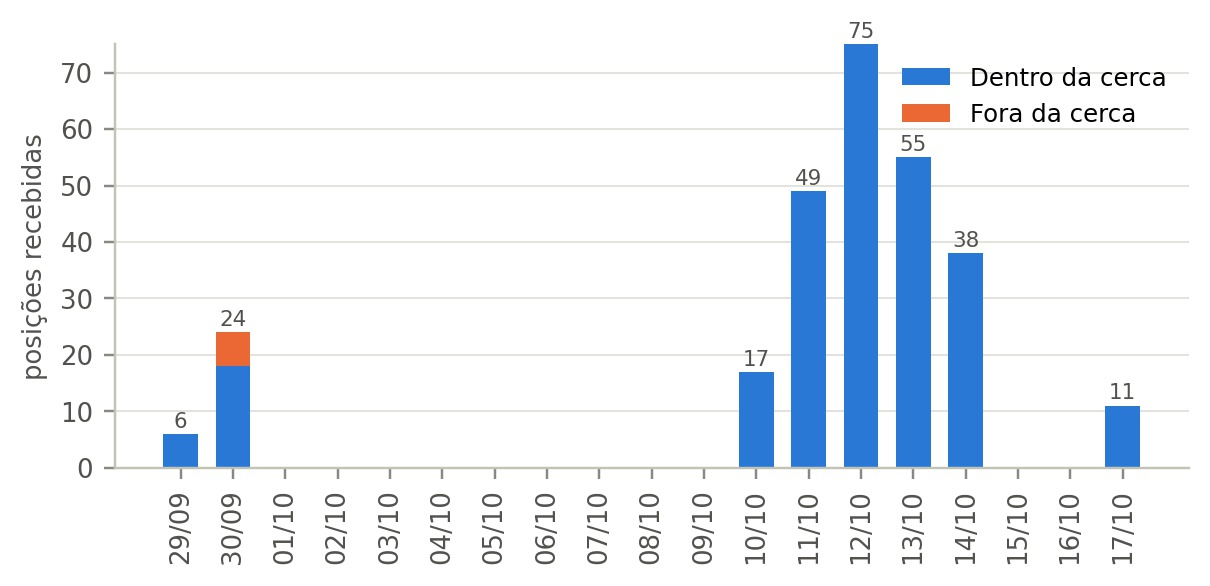
\includegraphics[width=\textwidth]{figuras/uc1_por_dia.jpg}
  \fonte{Elaborado pelo autor (2026).}
\end{figure}

A Figura~\ref{fig:uc1-intervalo} apresenta o intervalo entre posições consecutivas e a precisão informada pela rede em cada posição. O intervalo mediano foi de 16 min, e 90\% dos intervalos ficaram abaixo de 57 min; o maior intervalo, de 239 h, corresponde à lacuna entre 30/09 e 10/10. A precisão informada teve mediana de 75 m, e 46\% das posições chegaram com o valor máximo aceito pelo filtro do servidor, 100 m.

\begin{figure}[htb]
  \centering
  \caption{Intervalo entre posições consecutivas e precisão informada pela rede}
  \label{fig:uc1-intervalo}
  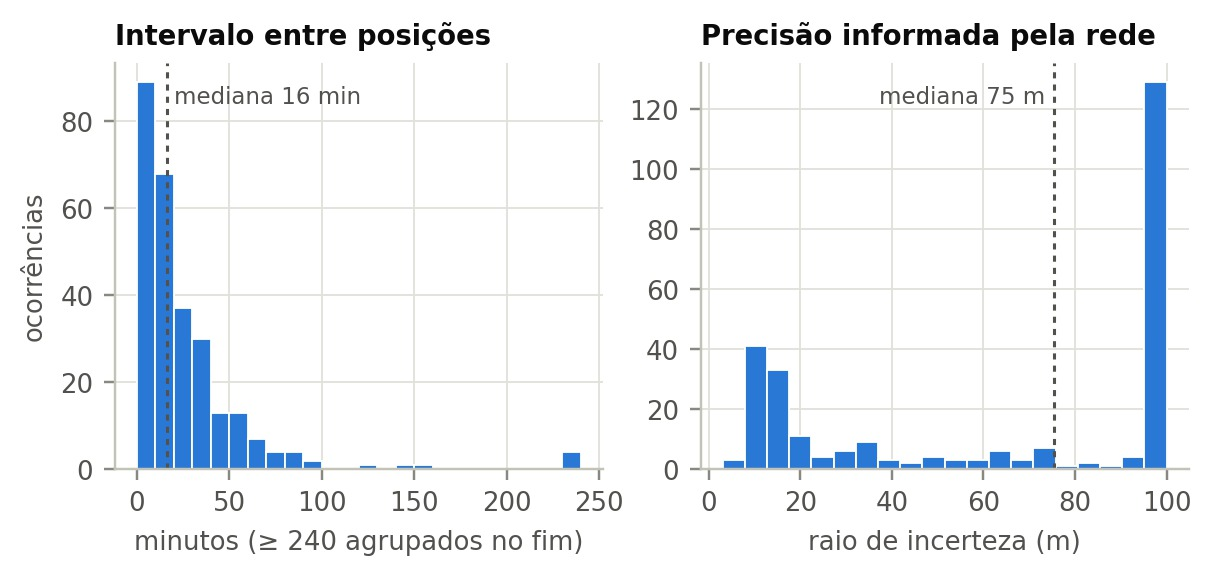
\includegraphics[width=\textwidth]{figuras/uc1_intervalo_precisao.jpg}
  \fonte{Elaborado pelo autor (2026).}
\end{figure}

\subsection{Incerteza da posição}
\label{sec:uc1-incerteza-posicao}

A incerteza foi avaliada pela análise de amostra única de \citeonline{moffat1988}: cada posição é uma leitura isolada, e a dispersão do sistema de medição é obtida de um experimento auxiliar feito em condição representativa. O experimento auxiliar foi o período de 10/10 a 17/10, com a \textit{tag} parada no mesmo ponto e 243 leituras. As coordenadas foram convertidas para metros nas direções leste ($x$) e norte ($y$), e o desvio-padrão amostral de cada direção foi $S_x = 9{,}6$~m e $S_y = 14{,}0$~m.

Com 242 graus de liberdade, a distribuição qui-quadrado limita o desvio-padrão da população a $0{,}92\,S \le \sigma \le 1{,}10\,S$, ao nível de 95\% \cite{moffat1988}. Foi adotado o valor mais provável, $\sigma = S$. A incerteza de uma leitura isolada, a 95\% de confiança (chance de 20 para 1), é
\begin{equation}
  \delta x = 2\sigma_x = 19{,}2~\text{m}, \qquad \delta y = 2\sigma_y = 27{,}9~\text{m}.
  \label{eq:uc1-incerteza-posicao}
\end{equation}
Com o limite superior de $\sigma$, os valores seriam 21,0 m e 30,6 m. Nos dados, 96,3\% das leituras ficaram dentro de $\pm\delta x$ e 92,2\% dentro de $\pm\delta y$. A distribuição não é gaussiana, pois 92\% das leituras na direção leste ficaram dentro de $\pm S_x$, e uma leitura isolada se afastou 121 m da média. A autocorrelação entre leituras consecutivas foi de $-0{,}001$ (leste) e $0{,}12$ (norte), e as leituras foram tratadas como independentes, condição exigida para a soma quadrática.

A Tabela~\ref{tab:uc1-ordens} separa a incerteza da posição nas três ordens de \citeonline{moffat1988}. A ordem zero corresponde à resolução dos valores recebidos, que chegam com $10^{-7}$ grau (cerca de 1,1 cm), e a incerteza instrumental é a metade da resolução \cite{poiate}. O horário de cada posição chega em segundos inteiros, com incerteza de 0,5 s. A primeira ordem é a dispersão medida no experimento auxiliar. Na ordem $N$ entraria o erro fixo da rede, isto é, a diferença entre a média das leituras e a posição verdadeira da \textit{tag}. Esse erro não foi medido, porque não havia uma referência de posição com incerteza menor; ele desloca todas as leituras da mesma forma, e por isso se cancela nas diferenças entre posições usadas na distância e na velocidade, mas afeta a verificação da cerca.

\begin{table}[htb]
  \centering
  \caption{Incerteza de uma posição a 95\% de confiança}
  \label{tab:uc1-ordens}
  \begin{tabular}{lrrl}
    \hline
    \textbf{Ordem} & \textbf{Leste (m)} & \textbf{Norte (m)} & \textbf{Origem} \\
    \hline
    Zero & 0,005 & 0,006 & resolução de $10^{-7}$ grau \\
    Primeira & 19,2 & 27,9 & experimento auxiliar, $2S$ \\
    $N$ & 19,2 & 27,9 & erro fixo da rede não avaliado \\
    \hline
  \end{tabular}
  \fonte{Elaborado pelo autor (2026).}
\end{table}

A ordem zero é cerca de 4 mil vezes menor que a primeira e foi desprezada, pois uma parcela menor que um terço da maior tem efeito pequeno na soma quadrática \cite{moffat1988}. Em 95,9\% das leituras paradas, a distância até a média ficou abaixo da precisão informada pela rede para aquela leitura, cuja mediana foi de 75 m. A precisão informada se comporta como um limite conservador, maior que a incerteza medida.

\subsection{Verificação da cerca com a incerteza}

A cerca virtual funciona como uma tolerância: a posição é aceita enquanto a distância $r$ até o centro não passa do raio $R = 310$~m. Seguindo \citeonline{poiate}, a incerteza de medição divide a faixa em três zonas. A zona de aceitação vai até $R - \delta r$, a zona de rejeição começa em $R + \delta r$ e, entre as duas, fica a zona de dúvida, onde a medição não permite afirmar se a \textit{tag} está dentro ou fora. A incerteza da distância ao centro vem da propagação das incertezas da Equação~\eqref{eq:uc1-incerteza-posicao}:
\begin{equation}
  \delta r = \sqrt{\left(\frac{x}{r}\,\delta x\right)^2 + \left(\frac{y}{r}\,\delta y\right)^2}.
  \label{eq:uc1-incerteza-raio}
\end{equation}

O maior valor de $\delta r$ entre as posições foi de 27,8 m, o que coloca a zona de dúvida entre 282 m e 338 m. A incerteza ficou abaixo de um décimo do intervalo de tolerância (31 m), critério de equilíbrio entre custo e qualidade recomendado por \citeonline{poiate}. A Figura~\ref{fig:uc1-zonas} mostra a distância de cada posição ao centro com as três zonas.

\begin{figure}[htb]
  \centering
  \caption{Distância das posições ao centro da cerca, com as zonas de aceitação, dúvida e rejeição}
  \label{fig:uc1-zonas}
  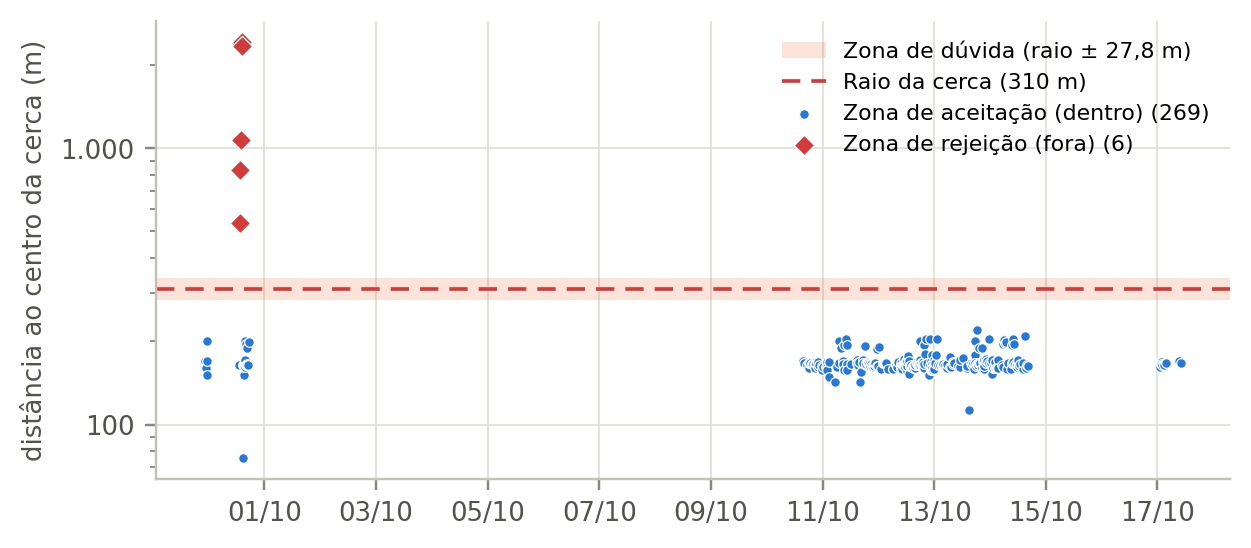
\includegraphics[width=\textwidth]{figuras/uc1_zonas.jpg}
  \fonte{Elaborado pelo autor (2026).}
\end{figure}

As 269 posições dentro da cerca ficaram a até 220 m do centro, na zona de aceitação. As seis posições de 30/09 ficaram a pelo menos 536 m, na zona de rejeição, e nenhuma posição caiu na zona de dúvida. O alerta de saída da cerca de 30/09 não depende, portanto, da incerteza da posição.

\subsection{Parâmetros calculados pelo site}

O site calcula, a partir das posições gravadas no banco, quatro parâmetros para o intervalo escolhido. A distância percorrida é a soma das distâncias entre posições consecutivas, $d = \sum_k s_k$. A velocidade média é essa distância dividida pelo tempo $T$ entre a primeira e a última posição. A velocidade máxima é a maior razão $s_k/\Delta t_k$ entre duas posições consecutivas. A aceleração média é a média das variações de velocidade entre trechos seguidos.

A incerteza desses resultados foi propagada pelo método da perturbação sequencial \cite{moffat1988}, aplicado à mesma função de cálculo do site. Cada entrada $X_i$ (latitude, longitude e horário de cada posição) foi aumentada e reduzida pela sua incerteza $\delta X_i$, uma de cada vez, e a contribuição $C_i$ foi tomada como a média de $|R_{i+} - R_0|$ e $|R_{i-} - R_0|$, porque o resultado não é linear nas posições. A incerteza do resultado é a soma quadrática das contribuições,
\begin{equation}
  \delta R = \sqrt{\sum_i C_i^2}, \qquad C_i \approx \frac{\partial R}{\partial X_i}\,\delta X_i,
  \label{eq:uc1-perturbacao}
\end{equation}
e tem o mesmo nível de confiança das entradas, 95\%. Para a velocidade média, a propagação analítica da apostila de \citeonline{poiate},
\begin{equation}
  \frac{\delta \bar v}{\bar v} = \sqrt{\left(\frac{\delta d}{d}\right)^2 + \left(\frac{\delta T}{T}\right)^2},
  \label{eq:uc1-vmed}
\end{equation}
com $\delta T = 1$~s (metade da resolução em cada extremo), deu o mesmo valor que a perturbação sequencial até a terceira casa. A parcela do horário foi desprezível em todos os resultados, exceto na velocidade máxima de 13/10, em que foi de 23 km/h contra 128 km/h da parcela das posições.

A soma de passos tem também um erro fixo, que \citeonline{moffat1988} classifica como erro conceitual: com a \textit{tag} parada, o ruído da posição gera passos de comprimento não nulo, e o site os soma como distância. Esse erro foi medido no experimento auxiliar, com 121 pares de leituras consecutivas sem leitura em comum. O passo médio foi de $(14{,}0 \pm 3{,}3)$~m, em que a incerteza é $t\,S/\sqrt{N}$, com $t = 1{,}98$ para 120 graus de liberdade. Para um intervalo com $k$ passos, o erro fixo é $B = k \times 14{,}0$~m, e a sua incerteza, $k \times 3{,}3$~m, somada de forma linear, porque o mesmo valor médio é usado em todos os passos. A distância corrigida é $d - B$, e a sua incerteza de ordem $N$ é a soma quadrática da incerteza propagada com a incerteza de $B$. Essa correção supõe a \textit{tag} parada em todos os passos e, nos dias com deslocamento, superestima o erro fixo. A velocidade média recebe a mesma correção, dividida por $T$.

A Figura~\ref{fig:uc1-parametros} apresenta, por dia, o valor calculado pelo site, a incerteza expandida e o erro fixo. Um valor foi considerado significativo quando superou a sua incerteza, isto é, quando a diferença em relação a zero (ou ao erro fixo, no caso da distância e da velocidade média) foi maior que a incerteza dessa diferença \cite{moffat1988}.

\begin{figure}[htb]
  \centering
  \caption{Parâmetros calculados pelo site por dia, com a incerteza expandida e o erro fixo}
  \label{fig:uc1-parametros}
  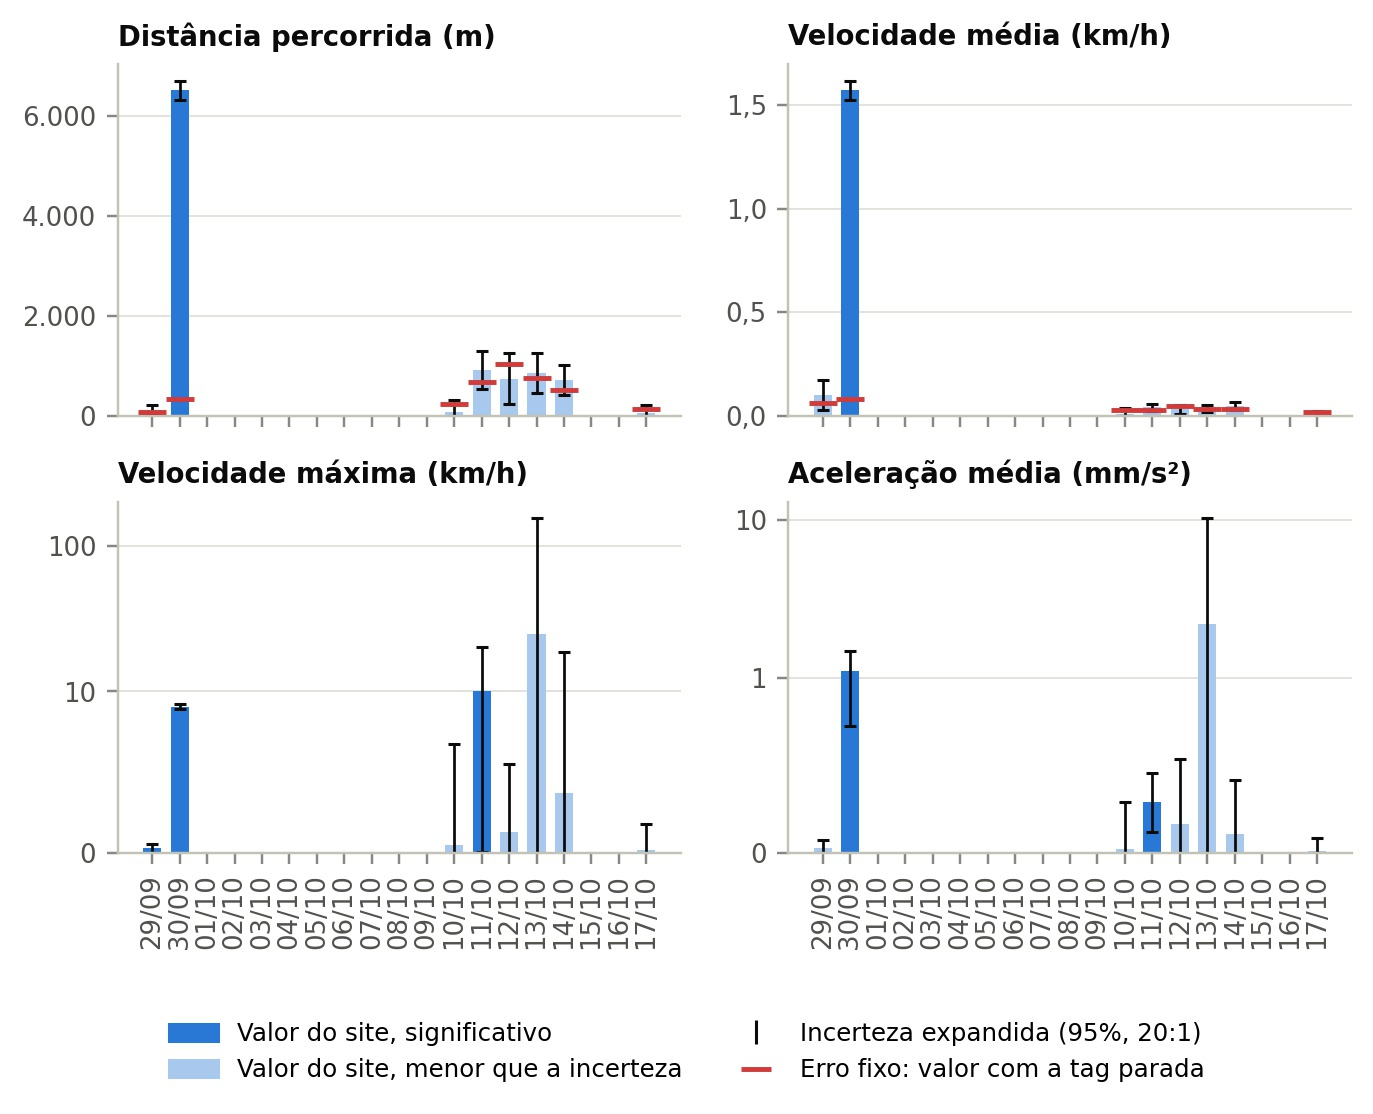
\includegraphics[width=\textwidth]{figuras/uc1_parametros.jpg}
  \fonte{Elaborado pelo autor (2026).}
\end{figure}

A Tabela~\ref{tab:uc1-dia30} reúne os resultados de 30/09, o dia com deslocamento, em 24 posições e 4 h 08 min. Todos os parâmetros foram significativos. A distância corrigida foi de $(6{,}19 \pm 0{,}19)$~km, com incerteza relativa de 3\%.

\begin{table}[htb]
  \centering
  \caption{Parâmetros de 30/09 a 95\% de confiança}
  \label{tab:uc1-dia30}
  \begin{tabular}{lrrr}
    \hline
    \textbf{Parâmetro} & \textbf{Valor do site} & \textbf{Erro fixo} & \textbf{Valor corrigido} \\
    \hline
    Distância percorrida & $(6{,}51 \pm 0{,}17)$ km & $(0{,}32 \pm 0{,}08)$ km & $(6{,}19 \pm 0{,}19)$ km \\
    Velocidade média & $(1{,}57 \pm 0{,}04)$ km/h & 0,08 km/h & $(1{,}50 \pm 0{,}05)$ km/h \\
    Velocidade máxima & $(9{,}0 \pm 0{,}2)$ km/h & --- & --- \\
    Aceleração média & $(1{,}1 \pm 0{,}4)$ mm/s² & --- & --- \\
    \hline
  \end{tabular}
  \fonte{Elaborado pelo autor (2026).}
\end{table}

Nos dias com a \textit{tag} parada, a distância corrigida foi compatível com zero. Em 11/10, por exemplo, o site somou 914 m, o erro fixo foi de 674 m e a distância corrigida, $(240 \pm 370)$~m. A velocidade máxima de 11/10, $(10 \pm 10)$~km/h, ficou no limite da significância, e a de 13/10, 24,7 km/h, teve incerteza de 130 km/h, porque vem de duas posições recebidas com poucos segundos de diferença. A Tabela~\ref{tab:uc1-total} reúne os parâmetros do intervalo total.

\begin{table}[htb]
  \centering
  \caption{Parâmetros calculados pelo site no intervalo total (29/09 a 17/10), a 95\% de confiança}
  \label{tab:uc1-total}
  \begin{tabular}{lrrr}
    \hline
    \textbf{Parâmetro} & \textbf{Valor do site} & \textbf{Erro fixo} & \textbf{Valor corrigido} \\
    \hline
    Distância percorrida & $(10{,}1 \pm 0{,}8)$ km & $(3{,}8 \pm 0{,}9)$ km & $(6{,}2 \pm 1{,}2)$ km \\
    Velocidade média & $(0{,}024 \pm 0{,}002)$ km/h & 0,009 km/h & $(0{,}015 \pm 0{,}003)$ km/h \\
    Velocidade máxima & $(25 \pm 130)$ km/h & --- & --- \\
    Aceleração média & $(0{,}7 \pm 1{,}7)$ mm/s² & --- & --- \\
    \hline
  \end{tabular}
  \fonte{Elaborado pelo autor (2026).}
\end{table}

A distância corrigida do intervalo total, $(6{,}2 \pm 1{,}2)$~km, coincide com a de 30/09: o restante dos 10,1 km somados pelo site corresponde ao ruído da posição nos dias parados. Um passo de comprimento próximo de zero tem incerteza de $\sqrt{2}\,\delta y = 39{,}5$~m, e 243 dos 274 passos do intervalo ficaram abaixo desse valor. A velocidade máxima e a aceleração média do intervalo total têm incerteza maior que o próprio valor e não permitem conclusões.

Com intervalos medianos de 16 min e incerteza de 19 m (leste) e 28 m (norte) a 95\% de confiança, a localização pela rede Find Hub atende à verificação da cerca virtual, sem posições na zona de dúvida. Para medir distância e velocidade em treinos, o cálculo do site precisaria descontar o erro fixo ou descartar passos menores que a incerteza de um passo, ou essas grandezas teriam de vir do acelerômetro.


% ---------------------------------------------------------------------
\section{Caso de uso 2: coleta biométrica}
\label{sec:res-biometria}

A Figura~\ref{fig:uc2-cobertura} mostra, para cada dia com o sensor ligado, quantos minutos têm leitura de cada sinal no servidor. O movimento somou 959 min e a temperatura 785 min. As leituras de frequência cardíaca somaram 304 s, distribuídos em oito janelas.

\begin{figure}[htb]
  \centering
  \caption{Minutos com leitura no servidor, por dia e por sinal}
  \label{fig:uc2-cobertura}
  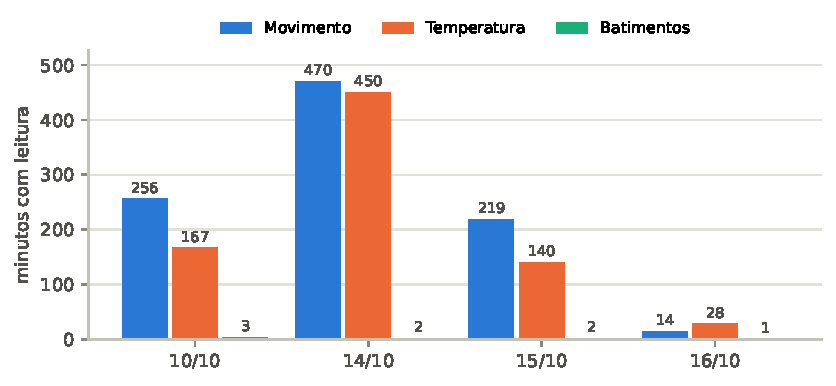
\includegraphics[width=0.95\linewidth]{figures/uc2_cobertura.pdf}
  \fonte{Elaborado pelo autor (2026).}
\end{figure}

A incerteza de cada sinal seguiu o mesmo procedimento do caso de uso 1 \cite{moffat1988}. A ordem zero é a metade da resolução do valor recebido \cite{poiate}; a primeira ordem é $2S$, com $S$ medido em um experimento auxiliar com o sensor em condição estável; o erro fixo vem da folha de dados ou de uma medição com valor conhecido; e a ordem $N$ é a soma quadrática dessas parcelas, a 95\% de confiança. A Tabela~\ref{tab:uc2-incerteza} resume os valores.

\begin{table}[htb]
  \centering
  \caption{Incerteza dos sinais biométricos a 95\% de confiança}
  \label{tab:uc2-incerteza}
  \begin{tabular}{lrrrr}
    \hline
    \textbf{Sinal} & \textbf{Ordem zero} & \textbf{1.ª ordem} & \textbf{Erro fixo} & \textbf{Ordem $N$} \\
    \hline
    Temperatura & 0,05 °C & 0,6 °C & 2,0 °C & 2,1 °C \\
    Movimento (minuto) & 0,00003 $g$ & 0,003 $g$ & 0,076 $g$ & 0,003 $g$\textsuperscript{a} \\
    Um batimento & 3,5 bpm & 6,0 bpm & não avaliado & 6,0 bpm \\
    Média de 16/10 & --- & 0,7 bpm & não avaliado & 0,7 bpm \\
    \hline
  \end{tabular}
  \fonte{Elaborado pelo autor (2026). \textsuperscript{a}Após descontar o erro fixo.}
\end{table}

\subsection{Frequência cardíaca}

O MAX30102 só calcula batimentos com pele encostada no sensor, e nos ensaios ele foi usado com o dedo do autor por poucos segundos. % CONFERIR
A Tabela~\ref{tab:bpm} lista as oito janelas. O sensor lê 25 vezes por segundo, e o intervalo entre dois picos tem resolução de 1/25 s. Pela propagação de $f = 60/T$, uma resolução $\delta T$ no período gera $\delta f = 60\,\delta T/T^2$ na frequência \cite{poiate}, valor que cresce com o quadrado da frequência: 3,5 bpm a 72 bpm e 21 bpm a 177 bpm.
% PROVISÓRIO: a janela de 16/10 00:03 tem valores fictícios (uc2.py, JANELA_PROVISORIA). Substituir pela medição real antes da entrega.

\begin{table}[htb]
  \centering
  \caption{Janelas com leitura de frequência cardíaca (bpm)}
  \label{tab:bpm}
  \begin{tabular}{lrrrrr}
    \hline
    \textbf{Início} & \textbf{Duração (s)} & \textbf{Média} & \textbf{Mínimo} & \textbf{Máximo} & \textbf{Resolução} \\
    \hline
    10/10 19:27 & 31 & 60,2 & 28,1 & 106,8 & 2,4 \\
    10/10 19:27 & 9 & 51,0 & 27,1 & 76,3 & 1,7 \\
    10/10 19:28 & 57 & 62,4 & 34,1 & 79,7 & 2,6 \\
    14/10 18:07 & 29 & 62,7 & 23,0 & 75,7 & 2,6 \\
    14/10 21:12 & 55 & 53,6 & 21,7 & 105,3 & 1,9 \\
    15/10 20:34 & 8 & 78,5 & 34,2 & 177,0 & 4,1 \\
    15/10 23:54 & 55 & 67,0 & 31,0 & 176,5 & 3,0 \\
    16/10 00:03 & 60 & 72,5 & 68,2 & 78,9 & 3,5 \\ % PROVISÓRIO
    \hline
  \end{tabular}
  \fonte{Elaborado pelo autor (2026). Resolução de um batimento na frequência média da janela.}
\end{table}

Nas sete primeiras janelas, os mínimos (22 a 34 bpm) e os máximos (até 177 bpm) se afastam da média muito mais que a resolução, o que mostra que o algoritmo de detecção de pulso aceitou picos falsos quando o dedo se moveu. O sensor dividia o barramento I2C com o MPU6050 em fios sem solda, e as falhas de contato desligaram a leitura de batimentos em parte do período. Na janela de 16/10, com 60 s de contato contínuo, a Figura~\ref{fig:uc2-batimentos} mostra os 73 batimentos. A média foi de $(72{,}5 \pm 0{,}7)$~bpm, com $S = 3{,}0$~bpm e $t = 1{,}99$ para 72 graus de liberdade, e a incerteza de um batimento isolado foi de $\pm 6{,}0$~bpm. Os valores se repetem em 68,2, 71,4, 75,0 e 78,9 bpm porque o período é contado em passos de 40 ms, e a resolução responde por boa parte da dispersão. O erro fixo do sensor exige comparação com um oxímetro de referência e não foi avaliado. % CONFERIR

\begin{figure}[htb]
  \centering
  \caption{Frequência de cada batimento na janela de 16/10, com a incerteza da média e de um batimento}
  \label{fig:uc2-batimentos}
  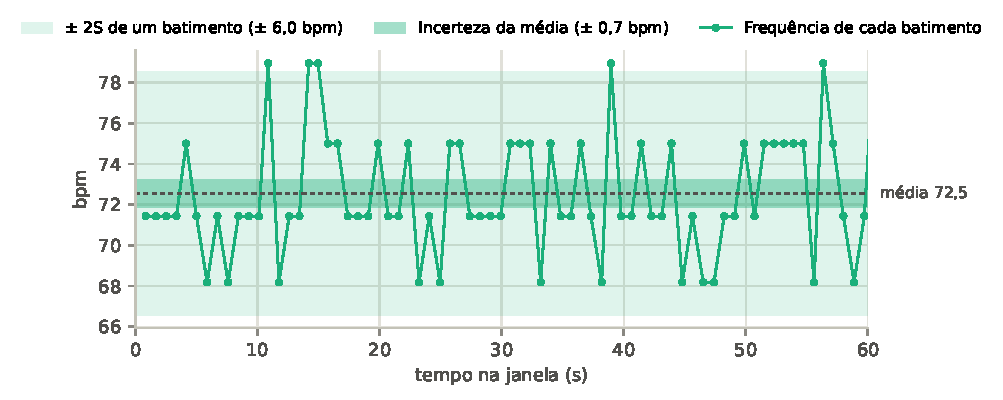
\includegraphics[width=0.95\linewidth]{figures/uc2_batimentos.pdf}
  \fonte{Elaborado pelo autor (2026).}
\end{figure}

\subsection{Temperatura}

A Figura~\ref{fig:uc2-temperatura} apresenta a temperatura como o portal a exibe, com a faixa de incerteza e os limites de alerta (35~°C e 40~°C) em vermelho. No dia 14/10 o DHT11 mediu o ar da sala, entre 24,0~°C e 27,9~°C em 450 leituras. A primeira ordem foi obtida das diferenças entre leituras sucessivas desse dia, que retiram a variação lenta da sala: $S = 0{,}30$~°C. A folha de dados do DHT11 informa exatidão de $\pm 2$~°C, adotada como erro fixo a 95\%. A ordem $N$ ficou em 2,1~°C, dominada pelo erro fixo.

\begin{figure}[htb]
  \centering
  \caption{Temperatura medida, incerteza e limites de alerta com as zonas de dúvida}
  \label{fig:uc2-temperatura}
  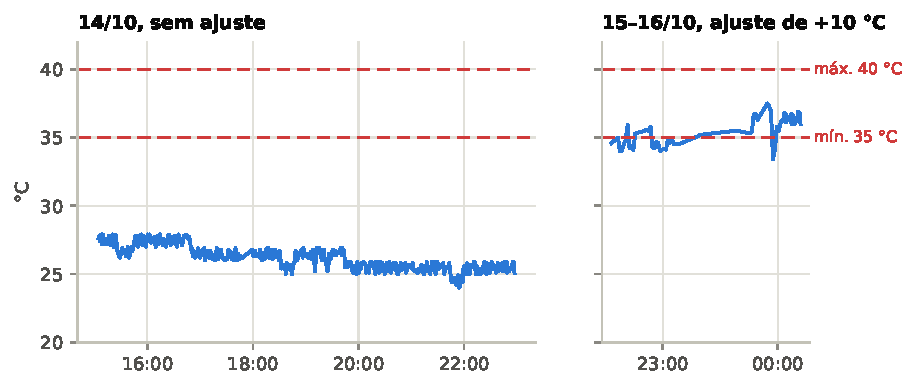
\includegraphics[width=0.95\linewidth]{figures/uc2_temperatura.pdf}
  \fonte{Elaborado pelo autor (2026).}
\end{figure}

Os limites de alerta formam uma tolerância de 5~°C. Pelo critério de \citeonline{poiate}, a incerteza deveria ficar abaixo de um décimo desse intervalo, 0,5~°C, e a do DHT11 é quatro vezes maior. A zona de aceitação fica reduzida a 37,1~°C a 37,9~°C, e as faixas de 32,9~°C a 37,1~°C e de 37,9~°C a 42,1~°C são zonas de dúvida, em que a medição não permite afirmar se a temperatura está dentro ou fora dos limites. As 450 leituras de 14/10 ficaram na zona de rejeição, abaixo do mínimo. Na noite de 15/10 foi salvo no portal um ajuste de +10~°C, usado para testar o caminho da calibração e não como correção medida. % CONFERIR
O sensor baixou o ajuste no envio seguinte e, a partir das 23h, as leituras passaram para a faixa de 33,4~°C a 37,5~°C: 47 das 49 leituras caíram na zona de dúvida e duas na zona de aceitação.

O teste confirma que o ajuste feito no portal chega ao sensor sem regravar o \textit{firmware} e passa a valer na comparação com os limites. O valor de +10~°C, porém, não corresponde a nenhuma referência e não reduz a incerteza: para uso no animal, o ajuste deve ser obtido comparando o sensor com um termômetro clínico, e um sensor com exatidão de 0,5~°C ou melhor atenderia ao critério de um décimo da tolerância.

\subsection{Movimento}

A Figura~\ref{fig:uc2-movimento} mostra a intensidade do movimento em 14/10, calculada como o afastamento do módulo da aceleração em relação a 1~$g$. Não havia limite de movimento configurado nesse dia. Nos 348 minutos com o sensor parado, a média por minuto foi de $(0{,}0761 \pm 0{,}0002)$~$g$, quando o esperado seria zero, com $S = 0{,}0016$~$g$ entre minutos. Nos 60 s mais estáveis das leituras brutas de 15/10, a 50 leituras/s, o módulo médio foi de 1,077~$g$, com $S = 0{,}003$~$g$ por leitura. O desvio de 0,076~$g$ é um erro fixo de escala do MPU6050, de 7,7\%, e é o motivo de o portal oferecer o ganho de calibração do movimento: com o ganho de $1/1{,}077$, a incerteza restante por minuto cai para 0,003~$g$. Sem a correção, o erro fixo precisa entrar na incerteza \cite{moffat1988}, e valores abaixo de cerca de 0,08~$g$ não se distinguem do sensor parado. Os picos de até 2,36~$g$ correspondem aos momentos em que o sensor foi manuseado e superam essa faixa com folga.

\begin{figure}[htb]
  \centering
  \caption{Intensidade do movimento por minuto em 14/10, com o erro fixo medido com o sensor parado (escala logarítmica acima de 0,1~$g$)}
  \label{fig:uc2-movimento}
  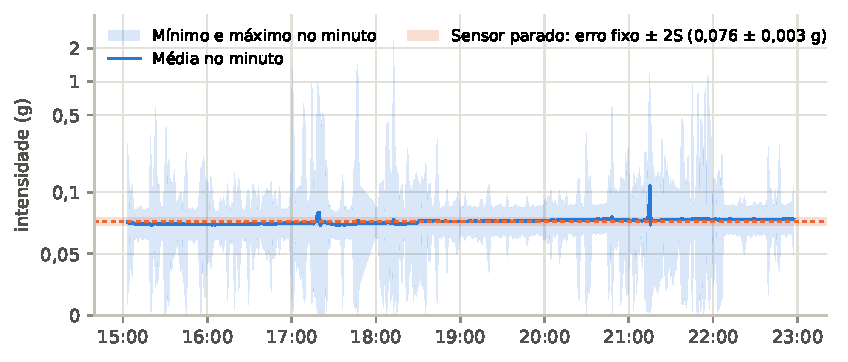
\includegraphics[width=0.95\linewidth]{figures/uc2_movimento.pdf}
  \fonte{Elaborado pelo autor (2026).}
\end{figure}

O envio de alertas por e-mail ao veterinário não foi avaliado, pois o servidor de e-mail (SMTP) não estava configurado no período. Os alertas pelo LED do sensor e pelo sino do portal foram verificados de forma visual, sem registro quantitativo. % CONFERIR

% ---------------------------------------------------------------------
\section{Caso de uso 3: detecção de padrões repetitivos}
\label{sec:res-padroes}

Os padrões ``Pulo'' e ``Volta'' foram avaliados em uma sessão de testes em 15/10, com 87,7 min de leituras do acelerômetro (263.089 amostras a 50 Hz). Nessa sessão o autor marcou no portal dez trechos, oito de Pulo e dois de Volta, que somam 22 s. Duas versões de detecção rodaram no sensor: até as 23h05, o modelo supervisionado treinado no servidor (floresta de 15 árvores de profundidade 4); depois desse horário, o detector físico descrito na metodologia.

A Figura~\ref{fig:uc3-sinal} mostra um trecho de 35 s com os três eixos, a marcação feita no portal (faixa cinza) e os eventos que o sensor registrou com o modelo supervisionado (linhas tracejadas).

\begin{figure}[htb]
  \centering
  \caption{Sinal do acelerômetro, trecho marcado como Pulo e eventos registrados pelo sensor}
  \label{fig:uc3-sinal}
  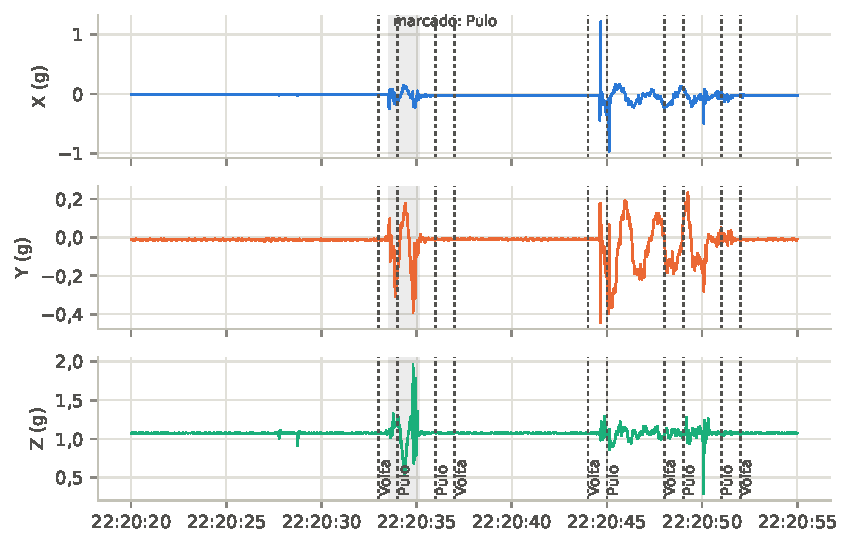
\includegraphics[width=0.95\linewidth]{figures/uc3_sinal_marcacoes.pdf}
  \fonte{Elaborado pelo autor (2026).}
\end{figure}

No trecho marcado, o eixo Z cai até cerca de 0,6~$g$ e sobe a quase 2~$g$, e o sensor registrou um Pulo dentro da marcação. O modelo, porém, também registrou eventos de Volta no mesmo instante e Pulos durante o manuseio seguinte, que não foi marcado. A Figura~\ref{fig:uc3-modelo} apresenta o desempenho do modelo supervisionado na validação feita pelo servidor no treino, deixando uma marcação de fora de cada vez.

\begin{figure}[htb]
  \centering
  \caption{Desempenho do modelo supervisionado na validação do treino}
  \label{fig:uc3-modelo}
  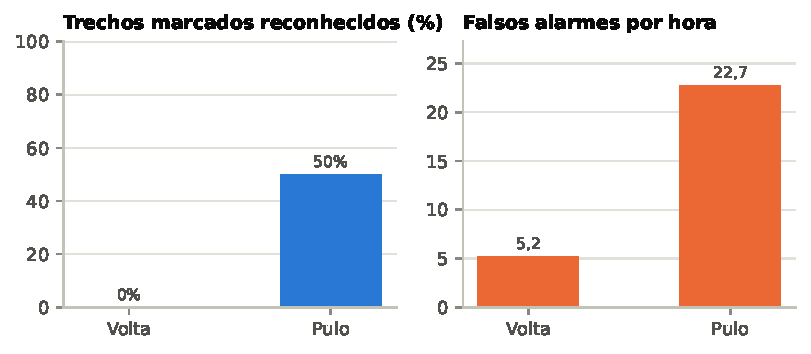
\includegraphics[width=0.95\linewidth]{figures/uc3_modelo_supervisionado.pdf}
  \fonte{Elaborado pelo autor (2026).}
\end{figure}

O modelo reconheceu 50\% dos trechos de Pulo, com 22,7 falsos alarmes por hora fora das marcações, e nenhum trecho de Volta. Com oito exemplos de Pulo (31 janelas) contra 3.000 janelas negativas, e dois exemplos de Volta, a base de treino é pequena demais para separar os padrões do manuseio comum do sensor. Esse resultado levou à troca do modelo supervisionado por um detector baseado na física do movimento, que não depende de exemplos marcados.

No detector físico, um salto é identificado pelo tempo $T$ em queda livre, em que o módulo da aceleração fica abaixo de 0,6~$g$. A altura vem da equação do lançamento vertical, $h = gT^2/8$, e o salto só é contado acima de 5~cm. A Figura~\ref{fig:uc3-voo} mostra os 20 voos com pelo menos 0,06 s encontrados ao reaplicar essa regra às leituras da sessão.

\begin{figure}[htb]
  \centering
  \caption{Altura estimada de cada voo pelo tempo em queda livre e limiar de contagem}
  \label{fig:uc3-voo}
  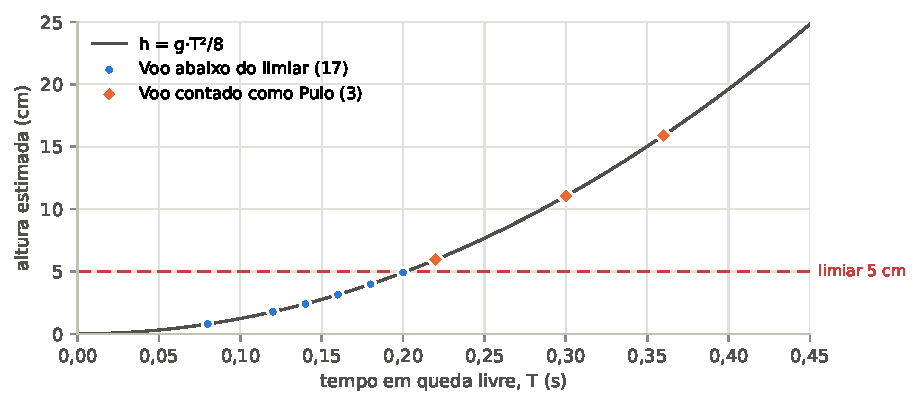
\includegraphics[width=0.95\linewidth]{figures/uc3_voo_altura.pdf}
  \fonte{Elaborado pelo autor (2026).}
\end{figure}

Três voos passaram do limiar, com 5,9 cm, 11 cm e 15,9 cm; os outros 17 ficaram entre 0,8 cm e 4,9 cm. Os oito trechos marcados como Pulo tiveram voos abaixo de 5 cm, de modo que nenhum deles foi contado. Os saltos do teste foram pequenos, feitos levantando e soltando a placa, e ficaram na faixa em que a regra não distingue um salto de um solavanco. Em um cavalo, um salto de 1 m corresponde a cerca de 0,9 s em queda livre, valor muito acima do ruído observado.

A Tabela~\ref{tab:uc3} compara as duas versões. A versão supervisionada é a que rodou no sensor até as 23h05; a física foi reaplicada às leituras da sessão inteira. Os eventos fora das marcações não equivalem a falsos alarmes, pois o autor não marcou todos os movimentos feitos durante a sessão.

\begin{table}[htb]
  \centering
  \caption{Marcações reconhecidas e eventos por versão de detecção na sessão de 15/10}
  \label{tab:uc3}
  \begin{tabular}{llrrr}
    \hline
    \textbf{Padrão} & \textbf{Versão} & \textbf{Marcações} & \textbf{Reconhecidas} & \textbf{Eventos} \\
    \hline
    Pulo  & Supervisionada (sensor) & 6 & 1 & 39 \\
    Volta & Supervisionada (sensor) & 2 & 0 & 42 \\
    Pulo  & Física (reaplicada) & 8 & 0 & 3 \\
    Volta & Física (reaplicada) & 2 & 2 & 22 \\
    \hline
  \end{tabular}
  \fonte{Elaborado pelo autor (2026).}
\end{table}

Para a Volta, o detector físico reconheceu os dois trechos marcados ao somar 360° de rotação do vetor horizontal da aceleração, e registrou 22 voltas na sessão, contra 42 do modelo supervisionado em um período menor. A reaplicação usou apenas o método do vetor horizontal, pois as leituras do giroscópio não ficam guardadas no servidor; no sensor, a volta também é contada pela rotação medida pelo giroscópio.

% ---------------------------------------------------------------------
\section{Caso de uso 4}
\label{sec:res-uc4}

% PENDENTE: resultados do caso de uso 4.
Os resultados deste caso de uso serão apresentados após a conclusão dos ensaios.

% ---------------------------------------------------------------------
\section{Síntese dos resultados}
\label{sec:res-sintese}

O protótipo coletou e enviou ao servidor 959 min de movimento e 785 min de temperatura em quatro dias, com as leituras guardadas no cartão SD entre um envio e outro. A localização pela rede Find Hub detectou a saída da cerca em 30/09, com posições a cada 16 min (mediana) e incerteza de 19 m (leste) e 28 m (norte) a 95\% de confiança. Com essa incerteza, o site soma cerca de 14 m por passo com a \textit{tag} parada, e a distância só foi significativa no dia com deslocamento. A calibração e os limites definidos no portal chegaram ao sensor sem regravar o \textit{firmware}. A frequência cardíaca teve 304 s de leitura, limitada pelo contato com a pele e pelas conexões do barramento I2C, e a janela com contato contínuo deu $(72{,}5 \pm 0{,}7)$~bpm. % PROVISÓRIO: valor da janela fictícia de 16/10
A temperatura teve incerteza de 2,1~°C, quatro vezes o recomendado para os limites de alerta, e o movimento, um erro fixo de 0,076~$g$ que o ganho de calibração corrige. Na detecção de padrões, o modelo supervisionado não atingiu desempenho útil com dez marcações, e o detector físico reconheceu as voltas marcadas, mas os saltos de teste ficaram abaixo do limiar de 5 cm. Os ensaios no animal são a próxima etapa para medir esses valores em condições reais.
. As figuras estão em figures/ (PDF vetorial; o PNG
% de mesmo nome serve para visualização).
%
% Estrutura (NBR 14724): o capítulo abre com as condições dos ensaios,
% segue a ordem dos casos de uso definidos na metodologia, cita cada
% figura e tabela no texto antes de ela aparecer, traz o título acima e a
% fonte abaixo, e discute cada resultado logo depois de apresentá-lo.
%
% Trechos marcados com "CONFERIR" dependem de informação que só o autor
% tem (condições dos ensaios). Revise antes de entregar.
%
% PROVISÓRIO: a janela de batimentos de 16/10 00:03 (caso de uso 2) tem
% valores fictícios. Substituir pela medição real antes da entrega.
% =====================================================================

\chapter{Resultados e discussão}
\label{cap:resultados}

Este capítulo apresenta os resultados obtidos com o protótipo entre 29 de setembro e 17 de outubro de 2026, organizados pelos casos de uso definidos na metodologia: localização (caso de uso 1), coleta biométrica (caso de uso 2), detecção de padrões repetitivos de movimento (caso de uso 3) e o caso de uso 4, ainda em andamento. Os dados foram extraídos da API do portal, a mesma que alimenta as telas do sistema, e processados por \textit{scripts} em Python para gerar as figuras.

Os ensaios foram feitos com o protótipo fora do animal: o sensor ficou sobre a bancada na maior parte do tempo e foi movimentado à mão nos testes de padrões, e a \textit{tag} de localização permaneceu em área urbana. % CONFERIR: condições dos ensaios
A Tabela~\ref{tab:condicoes} resume a configuração usada.

\begin{table}[htb]
  \centering
  \caption{Configuração do protótipo durante os ensaios}
  \label{tab:condicoes}
  \begin{tabular}{lp{8.5cm}}
    \hline
    \textbf{Item} & \textbf{Valor} \\
    \hline
    Microcontrolador & ESP32 DevKit \\
    Acelerômetro e giroscópio & MPU6050, 50 leituras/s \\
    Frequência cardíaca & MAX30102, 25 leituras/s \\
    Temperatura & DHT11, uma leitura a cada 20 s \\
    Armazenamento local & cartão microSD \\
    Intervalo de envio ao servidor & 180 s \\
    Localização & \textit{tag} BLE na rede Google Find Hub, consulta a cada 10 min \\
    Cerca virtual & círculo de 310 m de raio \\
    Período analisado & localização: 29/09 a 17/10/2026; sensor: 10/10 a 16/10/2026 \\
    \hline
  \end{tabular}
  \fonte{Elaborado pelo autor (2026).}
\end{table}

% ---------------------------------------------------------------------
% =====================================================================
% Caso de uso 1 (localização). Seção do capítulo de resultados, incluída
% em resultados.tex com % =====================================================================
% Caso de uso 1 (localização). Seção do capítulo de resultados, incluída
% em resultados.tex com % =====================================================================
% Caso de uso 1 (localização). Seção do capítulo de resultados, incluída
% em resultados.tex com \input{resultados_uc1}. Figuras em figuras/*.jpg.
% Incerteza: Moffat (1988) e Poiate Junior (apostila), chaves em referencias.bib.
% Trechos marcados com "CONFERIR" dependem de informação do autor.
% =====================================================================

\section{Caso de uso 1: localização}
\label{sec:res-localizacao}

O intervalo analisado vai de 29/09/2026 a 17/10/2026 e reúne 275 posições da \textit{tag}. As 32 primeiras, até 10/10, foram coletadas pela instância local do servidor, antes da implantação; as 243 seguintes, pela instância em produção. As duas instâncias usam o mesmo código de consulta e de filtragem. Entre 30/09 e 10/10 não há posições, porque o servidor local ficou desligado nesse período. % CONFERIR: motivo da lacuna
As posições estão em metros a partir do centro da cerca virtual, sem mapa de fundo, para não expor o endereço do local de teste.

A Figura~\ref{fig:uc1-trajeto} apresenta as posições em duas escalas. Em (a), o período de 10/10 a 17/10, com a \textit{tag} parada dentro da cerca de 310 m de raio. Em (b), o intervalo total, que inclui o deslocamento a pé feito pelo autor em 30/09.

\begin{figure}[htb]
  \centering
  \caption{Posições recebidas da \textit{tag} e cerca virtual: (a) período com a \textit{tag} parada; (b) intervalo total}
  \label{fig:uc1-trajeto}
  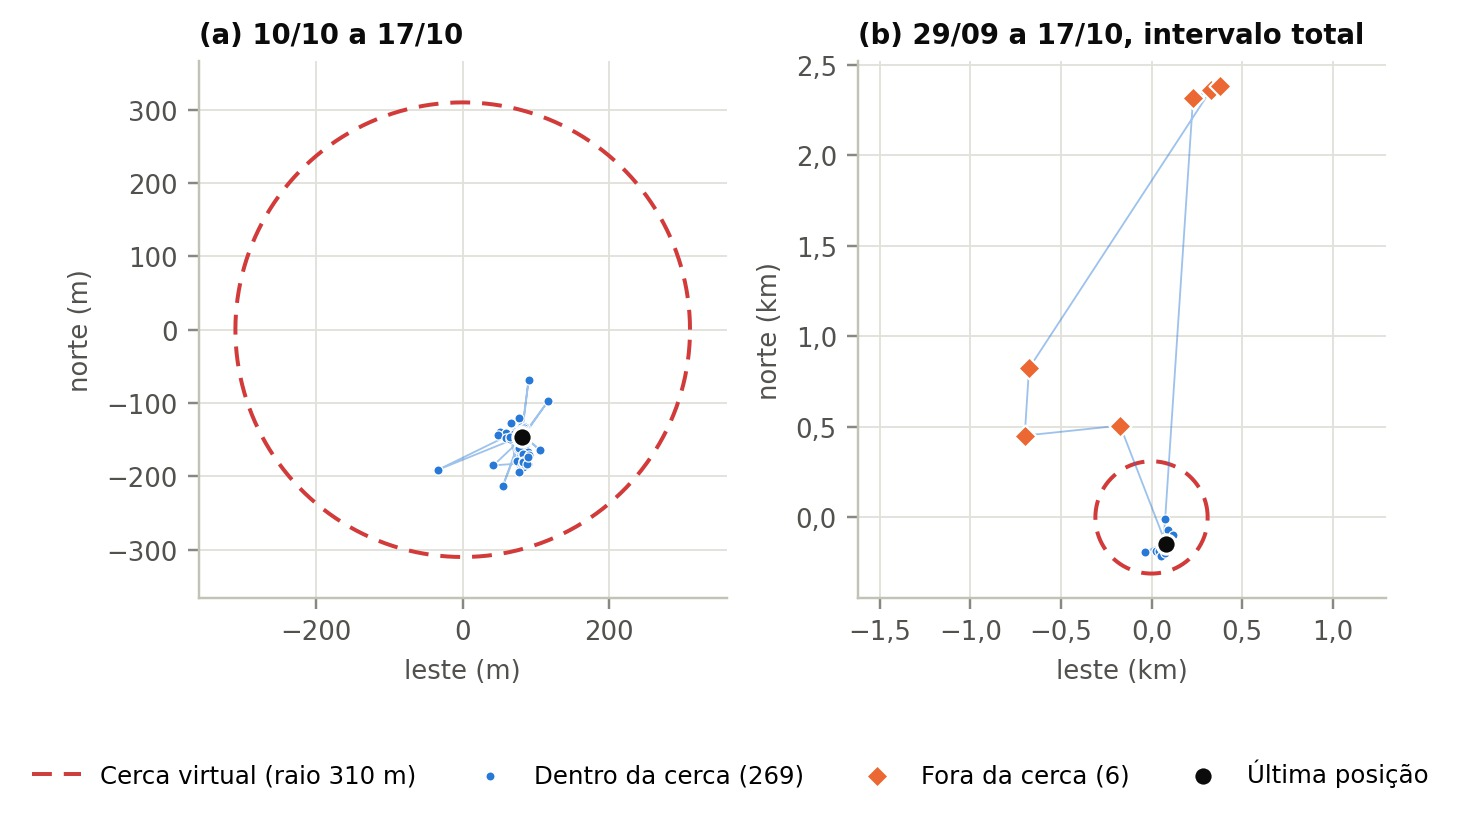
\includegraphics[width=\textwidth]{figuras/uc1_trajeto.jpg}
  \fonte{Elaborado pelo autor (2026).}
\end{figure}

Seis posições ficaram fora da cerca, todas em 30/09, entre 13h32 e 14h31, a até 2,41 km do centro. O site registrou o alerta de saída da cerca a partir da primeira delas: o cartão de localização do cavalo passou a indicar ``Fora da cerca'' e o alerta apareceu no sino do portal. Nas demais 269 posições a \textit{tag} estava dentro do raio.

A Figura~\ref{fig:uc1-dia} mostra quantas posições chegaram em cada dia. A quantidade variou de 6 a 75 por dia. A rede Find Hub depende de celulares Android que passem perto da \textit{tag}, e o servidor só registra o que a rede entrega.

\begin{figure}[htb]
  \centering
  \caption{Posições recebidas por dia, dentro e fora da cerca}
  \label{fig:uc1-dia}
  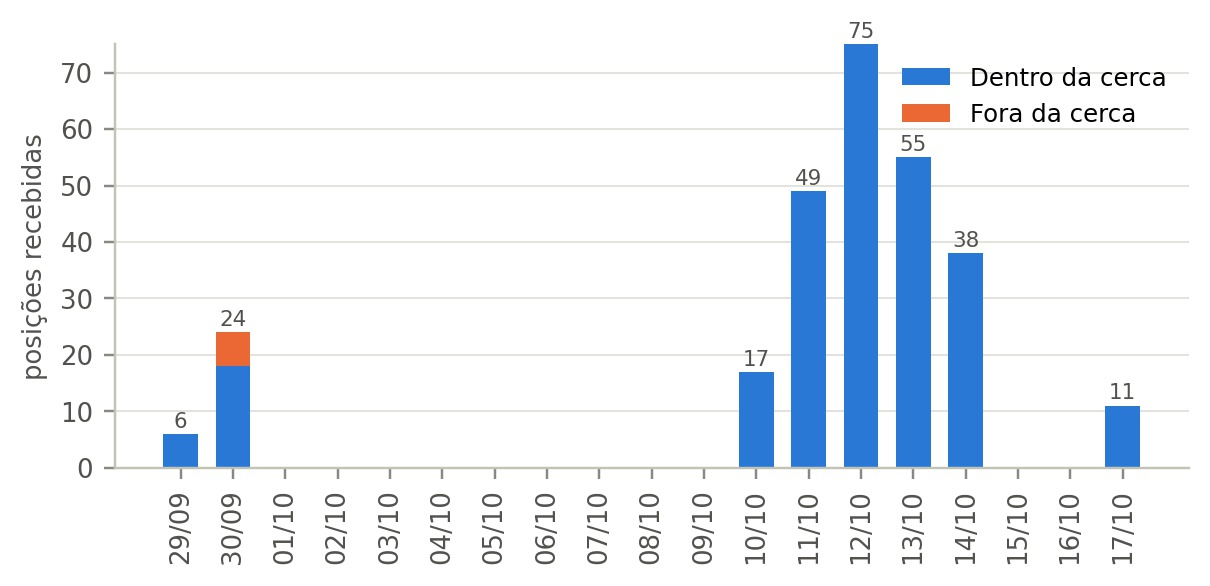
\includegraphics[width=\textwidth]{figuras/uc1_por_dia.jpg}
  \fonte{Elaborado pelo autor (2026).}
\end{figure}

A Figura~\ref{fig:uc1-intervalo} apresenta o intervalo entre posições consecutivas e a precisão informada pela rede em cada posição. O intervalo mediano foi de 16 min, e 90\% dos intervalos ficaram abaixo de 57 min; o maior intervalo, de 239 h, corresponde à lacuna entre 30/09 e 10/10. A precisão informada teve mediana de 75 m, e 46\% das posições chegaram com o valor máximo aceito pelo filtro do servidor, 100 m.

\begin{figure}[htb]
  \centering
  \caption{Intervalo entre posições consecutivas e precisão informada pela rede}
  \label{fig:uc1-intervalo}
  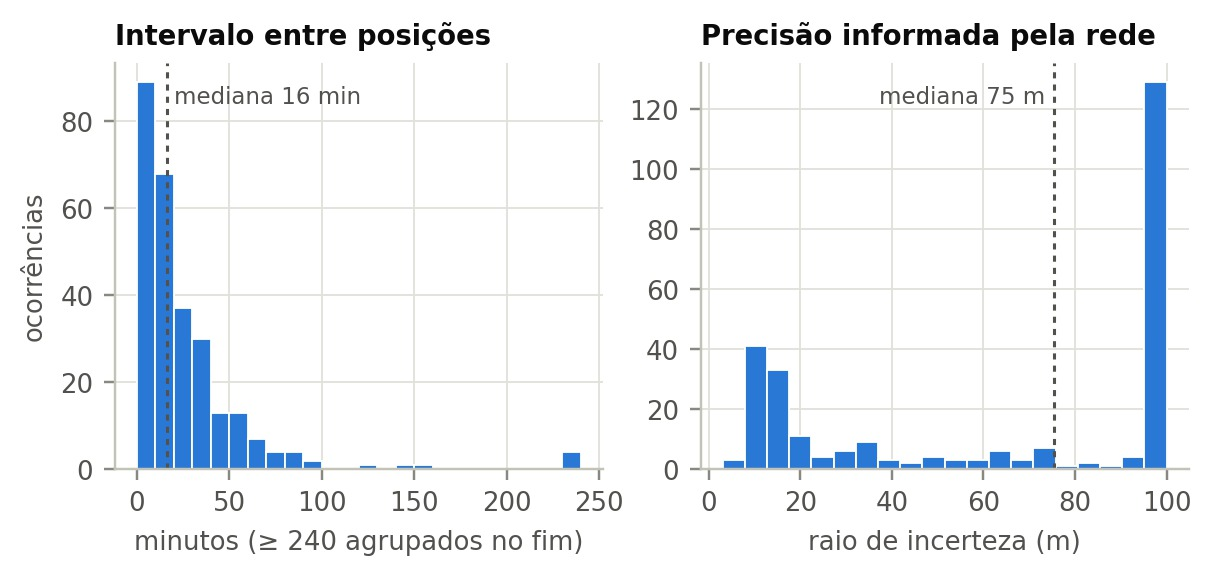
\includegraphics[width=\textwidth]{figuras/uc1_intervalo_precisao.jpg}
  \fonte{Elaborado pelo autor (2026).}
\end{figure}

\subsection{Incerteza da posição}
\label{sec:uc1-incerteza-posicao}

A incerteza foi avaliada pela análise de amostra única de \citeonline{moffat1988}: cada posição é uma leitura isolada, e a dispersão do sistema de medição é obtida de um experimento auxiliar feito em condição representativa. O experimento auxiliar foi o período de 10/10 a 17/10, com a \textit{tag} parada no mesmo ponto e 243 leituras. As coordenadas foram convertidas para metros nas direções leste ($x$) e norte ($y$), e o desvio-padrão amostral de cada direção foi $S_x = 9{,}6$~m e $S_y = 14{,}0$~m.

Com 242 graus de liberdade, a distribuição qui-quadrado limita o desvio-padrão da população a $0{,}92\,S \le \sigma \le 1{,}10\,S$, ao nível de 95\% \cite{moffat1988}. Foi adotado o valor mais provável, $\sigma = S$. A incerteza de uma leitura isolada, a 95\% de confiança (chance de 20 para 1), é
\begin{equation}
  \delta x = 2\sigma_x = 19{,}2~\text{m}, \qquad \delta y = 2\sigma_y = 27{,}9~\text{m}.
  \label{eq:uc1-incerteza-posicao}
\end{equation}
Com o limite superior de $\sigma$, os valores seriam 21,0 m e 30,6 m. Nos dados, 96,3\% das leituras ficaram dentro de $\pm\delta x$ e 92,2\% dentro de $\pm\delta y$. A distribuição não é gaussiana, pois 92\% das leituras na direção leste ficaram dentro de $\pm S_x$, e uma leitura isolada se afastou 121 m da média. A autocorrelação entre leituras consecutivas foi de $-0{,}001$ (leste) e $0{,}12$ (norte), e as leituras foram tratadas como independentes, condição exigida para a soma quadrática.

A Tabela~\ref{tab:uc1-ordens} separa a incerteza da posição nas três ordens de \citeonline{moffat1988}. A ordem zero corresponde à resolução dos valores recebidos, que chegam com $10^{-7}$ grau (cerca de 1,1 cm), e a incerteza instrumental é a metade da resolução \cite{poiate}. O horário de cada posição chega em segundos inteiros, com incerteza de 0,5 s. A primeira ordem é a dispersão medida no experimento auxiliar. Na ordem $N$ entraria o erro fixo da rede, isto é, a diferença entre a média das leituras e a posição verdadeira da \textit{tag}. Esse erro não foi medido, porque não havia uma referência de posição com incerteza menor; ele desloca todas as leituras da mesma forma, e por isso se cancela nas diferenças entre posições usadas na distância e na velocidade, mas afeta a verificação da cerca.

\begin{table}[htb]
  \centering
  \caption{Incerteza de uma posição a 95\% de confiança}
  \label{tab:uc1-ordens}
  \begin{tabular}{lrrl}
    \hline
    \textbf{Ordem} & \textbf{Leste (m)} & \textbf{Norte (m)} & \textbf{Origem} \\
    \hline
    Zero & 0,005 & 0,006 & resolução de $10^{-7}$ grau \\
    Primeira & 19,2 & 27,9 & experimento auxiliar, $2S$ \\
    $N$ & 19,2 & 27,9 & erro fixo da rede não avaliado \\
    \hline
  \end{tabular}
  \fonte{Elaborado pelo autor (2026).}
\end{table}

A ordem zero é cerca de 4 mil vezes menor que a primeira e foi desprezada, pois uma parcela menor que um terço da maior tem efeito pequeno na soma quadrática \cite{moffat1988}. Em 95,9\% das leituras paradas, a distância até a média ficou abaixo da precisão informada pela rede para aquela leitura, cuja mediana foi de 75 m. A precisão informada se comporta como um limite conservador, maior que a incerteza medida.

\subsection{Verificação da cerca com a incerteza}

A cerca virtual funciona como uma tolerância: a posição é aceita enquanto a distância $r$ até o centro não passa do raio $R = 310$~m. Seguindo \citeonline{poiate}, a incerteza de medição divide a faixa em três zonas. A zona de aceitação vai até $R - \delta r$, a zona de rejeição começa em $R + \delta r$ e, entre as duas, fica a zona de dúvida, onde a medição não permite afirmar se a \textit{tag} está dentro ou fora. A incerteza da distância ao centro vem da propagação das incertezas da Equação~\eqref{eq:uc1-incerteza-posicao}:
\begin{equation}
  \delta r = \sqrt{\left(\frac{x}{r}\,\delta x\right)^2 + \left(\frac{y}{r}\,\delta y\right)^2}.
  \label{eq:uc1-incerteza-raio}
\end{equation}

O maior valor de $\delta r$ entre as posições foi de 27,8 m, o que coloca a zona de dúvida entre 282 m e 338 m. A incerteza ficou abaixo de um décimo do intervalo de tolerância (31 m), critério de equilíbrio entre custo e qualidade recomendado por \citeonline{poiate}. A Figura~\ref{fig:uc1-zonas} mostra a distância de cada posição ao centro com as três zonas.

\begin{figure}[htb]
  \centering
  \caption{Distância das posições ao centro da cerca, com as zonas de aceitação, dúvida e rejeição}
  \label{fig:uc1-zonas}
  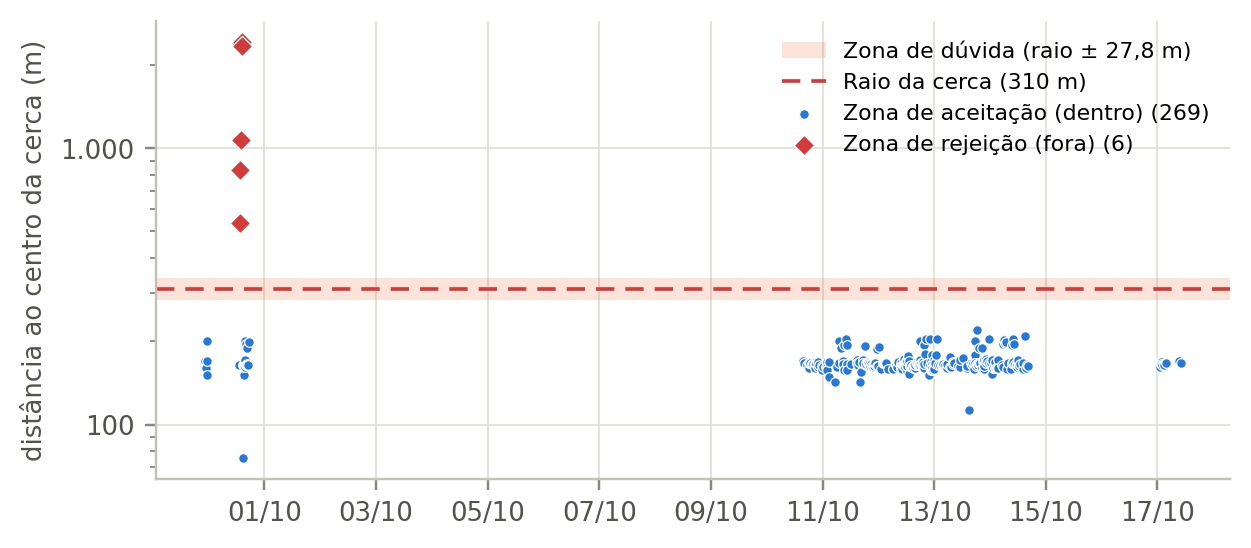
\includegraphics[width=\textwidth]{figuras/uc1_zonas.jpg}
  \fonte{Elaborado pelo autor (2026).}
\end{figure}

As 269 posições dentro da cerca ficaram a até 220 m do centro, na zona de aceitação. As seis posições de 30/09 ficaram a pelo menos 536 m, na zona de rejeição, e nenhuma posição caiu na zona de dúvida. O alerta de saída da cerca de 30/09 não depende, portanto, da incerteza da posição.

\subsection{Parâmetros calculados pelo site}

O site calcula, a partir das posições gravadas no banco, quatro parâmetros para o intervalo escolhido. A distância percorrida é a soma das distâncias entre posições consecutivas, $d = \sum_k s_k$. A velocidade média é essa distância dividida pelo tempo $T$ entre a primeira e a última posição. A velocidade máxima é a maior razão $s_k/\Delta t_k$ entre duas posições consecutivas. A aceleração média é a média das variações de velocidade entre trechos seguidos.

A incerteza desses resultados foi propagada pelo método da perturbação sequencial \cite{moffat1988}, aplicado à mesma função de cálculo do site. Cada entrada $X_i$ (latitude, longitude e horário de cada posição) foi aumentada e reduzida pela sua incerteza $\delta X_i$, uma de cada vez, e a contribuição $C_i$ foi tomada como a média de $|R_{i+} - R_0|$ e $|R_{i-} - R_0|$, porque o resultado não é linear nas posições. A incerteza do resultado é a soma quadrática das contribuições,
\begin{equation}
  \delta R = \sqrt{\sum_i C_i^2}, \qquad C_i \approx \frac{\partial R}{\partial X_i}\,\delta X_i,
  \label{eq:uc1-perturbacao}
\end{equation}
e tem o mesmo nível de confiança das entradas, 95\%. Para a velocidade média, a propagação analítica da apostila de \citeonline{poiate},
\begin{equation}
  \frac{\delta \bar v}{\bar v} = \sqrt{\left(\frac{\delta d}{d}\right)^2 + \left(\frac{\delta T}{T}\right)^2},
  \label{eq:uc1-vmed}
\end{equation}
com $\delta T = 1$~s (metade da resolução em cada extremo), deu o mesmo valor que a perturbação sequencial até a terceira casa. A parcela do horário foi desprezível em todos os resultados, exceto na velocidade máxima de 13/10, em que foi de 23 km/h contra 128 km/h da parcela das posições.

A soma de passos tem também um erro fixo, que \citeonline{moffat1988} classifica como erro conceitual: com a \textit{tag} parada, o ruído da posição gera passos de comprimento não nulo, e o site os soma como distância. Esse erro foi medido no experimento auxiliar, com 121 pares de leituras consecutivas sem leitura em comum. O passo médio foi de $(14{,}0 \pm 3{,}3)$~m, em que a incerteza é $t\,S/\sqrt{N}$, com $t = 1{,}98$ para 120 graus de liberdade. Para um intervalo com $k$ passos, o erro fixo é $B = k \times 14{,}0$~m, e a sua incerteza, $k \times 3{,}3$~m, somada de forma linear, porque o mesmo valor médio é usado em todos os passos. A distância corrigida é $d - B$, e a sua incerteza de ordem $N$ é a soma quadrática da incerteza propagada com a incerteza de $B$. Essa correção supõe a \textit{tag} parada em todos os passos e, nos dias com deslocamento, superestima o erro fixo. A velocidade média recebe a mesma correção, dividida por $T$.

A Figura~\ref{fig:uc1-parametros} apresenta, por dia, o valor calculado pelo site, a incerteza expandida e o erro fixo. Um valor foi considerado significativo quando superou a sua incerteza, isto é, quando a diferença em relação a zero (ou ao erro fixo, no caso da distância e da velocidade média) foi maior que a incerteza dessa diferença \cite{moffat1988}.

\begin{figure}[htb]
  \centering
  \caption{Parâmetros calculados pelo site por dia, com a incerteza expandida e o erro fixo}
  \label{fig:uc1-parametros}
  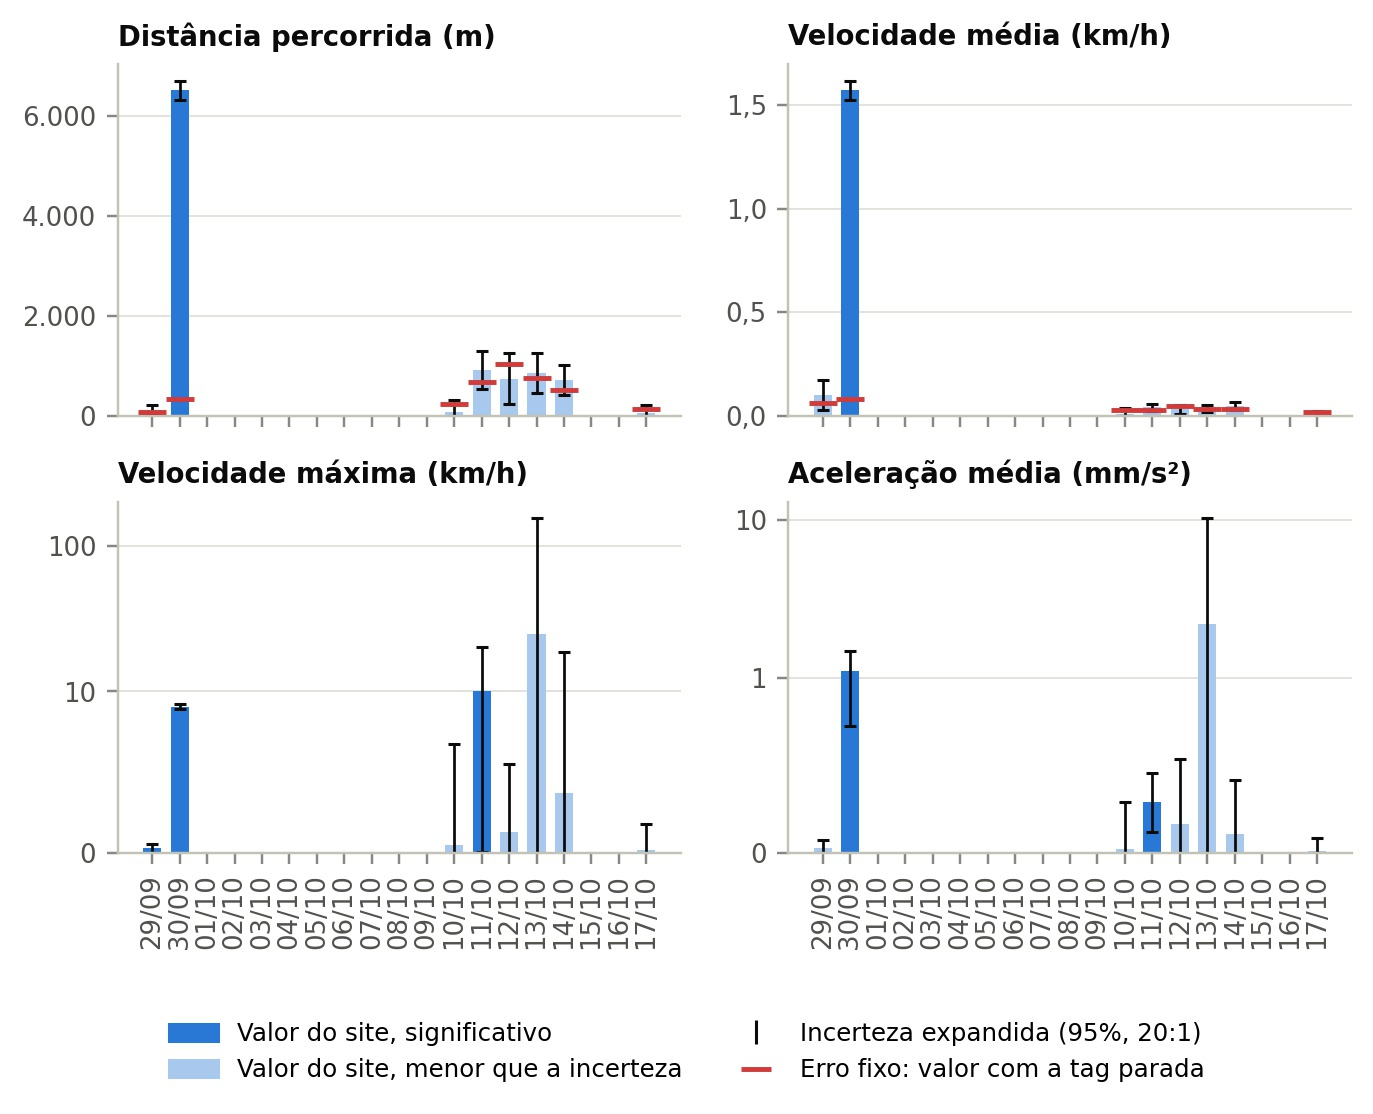
\includegraphics[width=\textwidth]{figuras/uc1_parametros.jpg}
  \fonte{Elaborado pelo autor (2026).}
\end{figure}

A Tabela~\ref{tab:uc1-dia30} reúne os resultados de 30/09, o dia com deslocamento, em 24 posições e 4 h 08 min. Todos os parâmetros foram significativos. A distância corrigida foi de $(6{,}19 \pm 0{,}19)$~km, com incerteza relativa de 3\%.

\begin{table}[htb]
  \centering
  \caption{Parâmetros de 30/09 a 95\% de confiança}
  \label{tab:uc1-dia30}
  \begin{tabular}{lrrr}
    \hline
    \textbf{Parâmetro} & \textbf{Valor do site} & \textbf{Erro fixo} & \textbf{Valor corrigido} \\
    \hline
    Distância percorrida & $(6{,}51 \pm 0{,}17)$ km & $(0{,}32 \pm 0{,}08)$ km & $(6{,}19 \pm 0{,}19)$ km \\
    Velocidade média & $(1{,}57 \pm 0{,}04)$ km/h & 0,08 km/h & $(1{,}50 \pm 0{,}05)$ km/h \\
    Velocidade máxima & $(9{,}0 \pm 0{,}2)$ km/h & --- & --- \\
    Aceleração média & $(1{,}1 \pm 0{,}4)$ mm/s² & --- & --- \\
    \hline
  \end{tabular}
  \fonte{Elaborado pelo autor (2026).}
\end{table}

Nos dias com a \textit{tag} parada, a distância corrigida foi compatível com zero. Em 11/10, por exemplo, o site somou 914 m, o erro fixo foi de 674 m e a distância corrigida, $(240 \pm 370)$~m. A velocidade máxima de 11/10, $(10 \pm 10)$~km/h, ficou no limite da significância, e a de 13/10, 24,7 km/h, teve incerteza de 130 km/h, porque vem de duas posições recebidas com poucos segundos de diferença. A Tabela~\ref{tab:uc1-total} reúne os parâmetros do intervalo total.

\begin{table}[htb]
  \centering
  \caption{Parâmetros calculados pelo site no intervalo total (29/09 a 17/10), a 95\% de confiança}
  \label{tab:uc1-total}
  \begin{tabular}{lrrr}
    \hline
    \textbf{Parâmetro} & \textbf{Valor do site} & \textbf{Erro fixo} & \textbf{Valor corrigido} \\
    \hline
    Distância percorrida & $(10{,}1 \pm 0{,}8)$ km & $(3{,}8 \pm 0{,}9)$ km & $(6{,}2 \pm 1{,}2)$ km \\
    Velocidade média & $(0{,}024 \pm 0{,}002)$ km/h & 0,009 km/h & $(0{,}015 \pm 0{,}003)$ km/h \\
    Velocidade máxima & $(25 \pm 130)$ km/h & --- & --- \\
    Aceleração média & $(0{,}7 \pm 1{,}7)$ mm/s² & --- & --- \\
    \hline
  \end{tabular}
  \fonte{Elaborado pelo autor (2026).}
\end{table}

A distância corrigida do intervalo total, $(6{,}2 \pm 1{,}2)$~km, coincide com a de 30/09: o restante dos 10,1 km somados pelo site corresponde ao ruído da posição nos dias parados. Um passo de comprimento próximo de zero tem incerteza de $\sqrt{2}\,\delta y = 39{,}5$~m, e 243 dos 274 passos do intervalo ficaram abaixo desse valor. A velocidade máxima e a aceleração média do intervalo total têm incerteza maior que o próprio valor e não permitem conclusões.

Com intervalos medianos de 16 min e incerteza de 19 m (leste) e 28 m (norte) a 95\% de confiança, a localização pela rede Find Hub atende à verificação da cerca virtual, sem posições na zona de dúvida. Para medir distância e velocidade em treinos, o cálculo do site precisaria descontar o erro fixo ou descartar passos menores que a incerteza de um passo, ou essas grandezas teriam de vir do acelerômetro.
. Figuras em figuras/*.jpg.
% Incerteza: Moffat (1988) e Poiate Junior (apostila), chaves em referencias.bib.
% Trechos marcados com "CONFERIR" dependem de informação do autor.
% =====================================================================

\section{Caso de uso 1: localização}
\label{sec:res-localizacao}

O intervalo analisado vai de 29/09/2026 a 17/10/2026 e reúne 275 posições da \textit{tag}. As 32 primeiras, até 10/10, foram coletadas pela instância local do servidor, antes da implantação; as 243 seguintes, pela instância em produção. As duas instâncias usam o mesmo código de consulta e de filtragem. Entre 30/09 e 10/10 não há posições, porque o servidor local ficou desligado nesse período. % CONFERIR: motivo da lacuna
As posições estão em metros a partir do centro da cerca virtual, sem mapa de fundo, para não expor o endereço do local de teste.

A Figura~\ref{fig:uc1-trajeto} apresenta as posições em duas escalas. Em (a), o período de 10/10 a 17/10, com a \textit{tag} parada dentro da cerca de 310 m de raio. Em (b), o intervalo total, que inclui o deslocamento a pé feito pelo autor em 30/09.

\begin{figure}[htb]
  \centering
  \caption{Posições recebidas da \textit{tag} e cerca virtual: (a) período com a \textit{tag} parada; (b) intervalo total}
  \label{fig:uc1-trajeto}
  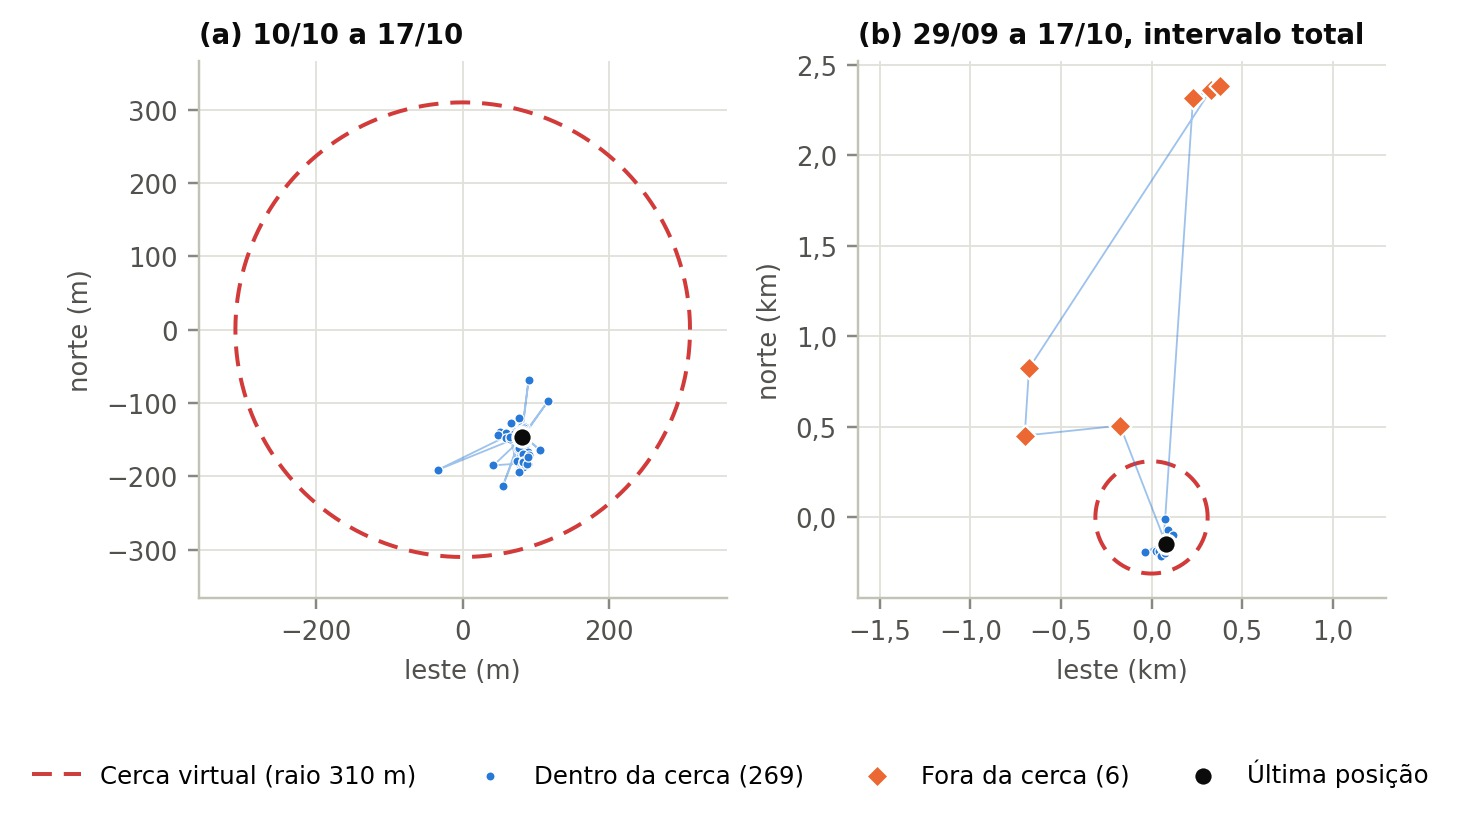
\includegraphics[width=\textwidth]{figuras/uc1_trajeto.jpg}
  \fonte{Elaborado pelo autor (2026).}
\end{figure}

Seis posições ficaram fora da cerca, todas em 30/09, entre 13h32 e 14h31, a até 2,41 km do centro. O site registrou o alerta de saída da cerca a partir da primeira delas: o cartão de localização do cavalo passou a indicar ``Fora da cerca'' e o alerta apareceu no sino do portal. Nas demais 269 posições a \textit{tag} estava dentro do raio.

A Figura~\ref{fig:uc1-dia} mostra quantas posições chegaram em cada dia. A quantidade variou de 6 a 75 por dia. A rede Find Hub depende de celulares Android que passem perto da \textit{tag}, e o servidor só registra o que a rede entrega.

\begin{figure}[htb]
  \centering
  \caption{Posições recebidas por dia, dentro e fora da cerca}
  \label{fig:uc1-dia}
  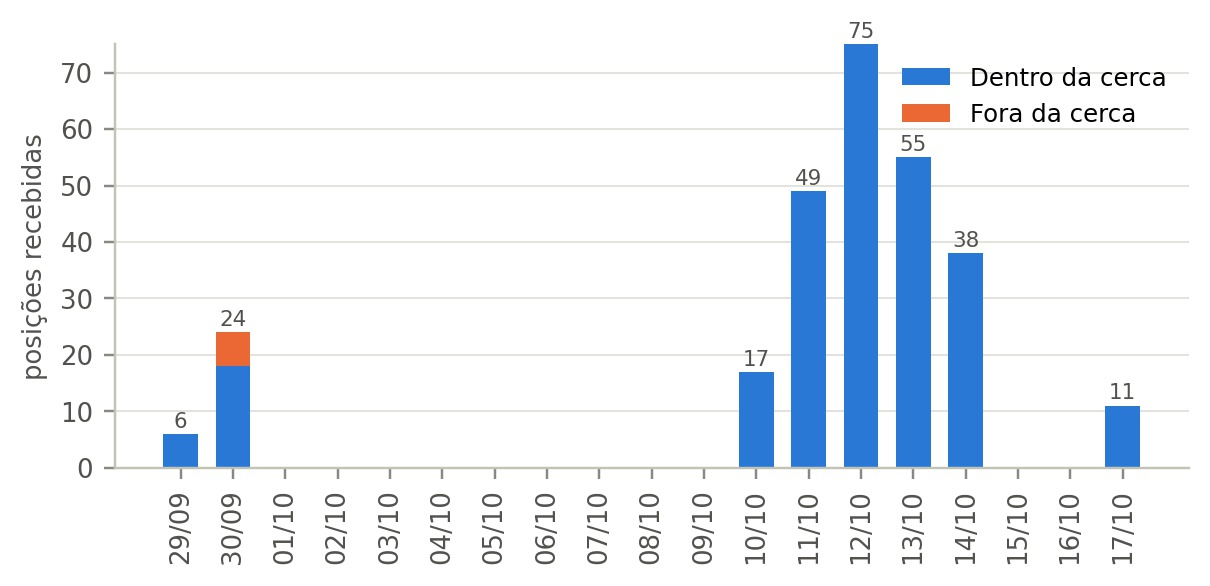
\includegraphics[width=\textwidth]{figuras/uc1_por_dia.jpg}
  \fonte{Elaborado pelo autor (2026).}
\end{figure}

A Figura~\ref{fig:uc1-intervalo} apresenta o intervalo entre posições consecutivas e a precisão informada pela rede em cada posição. O intervalo mediano foi de 16 min, e 90\% dos intervalos ficaram abaixo de 57 min; o maior intervalo, de 239 h, corresponde à lacuna entre 30/09 e 10/10. A precisão informada teve mediana de 75 m, e 46\% das posições chegaram com o valor máximo aceito pelo filtro do servidor, 100 m.

\begin{figure}[htb]
  \centering
  \caption{Intervalo entre posições consecutivas e precisão informada pela rede}
  \label{fig:uc1-intervalo}
  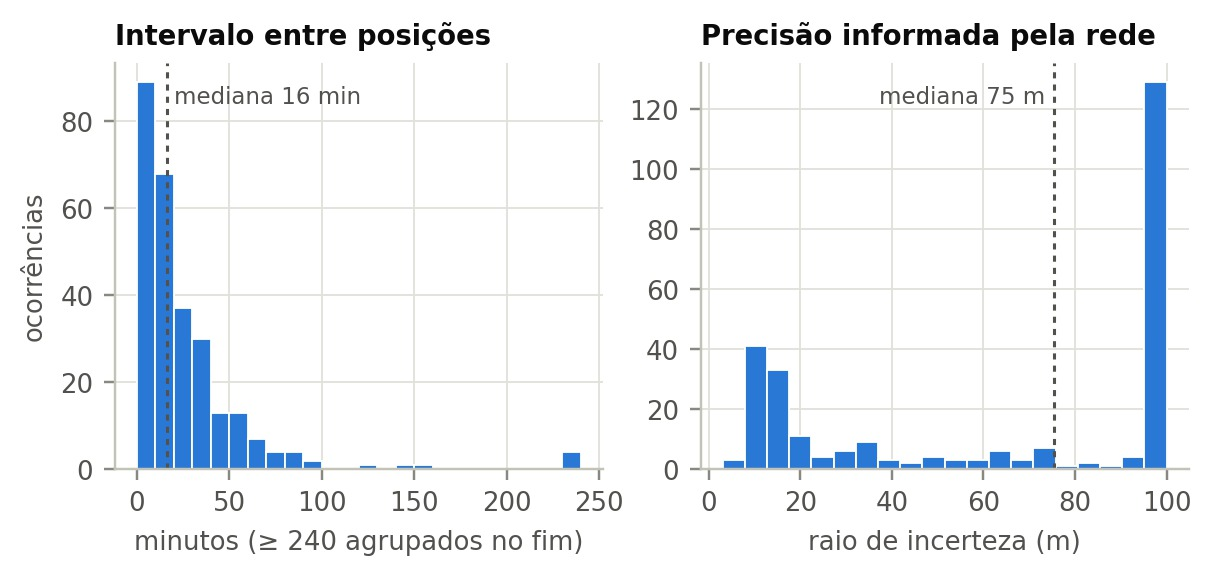
\includegraphics[width=\textwidth]{figuras/uc1_intervalo_precisao.jpg}
  \fonte{Elaborado pelo autor (2026).}
\end{figure}

\subsection{Incerteza da posição}
\label{sec:uc1-incerteza-posicao}

A incerteza foi avaliada pela análise de amostra única de \citeonline{moffat1988}: cada posição é uma leitura isolada, e a dispersão do sistema de medição é obtida de um experimento auxiliar feito em condição representativa. O experimento auxiliar foi o período de 10/10 a 17/10, com a \textit{tag} parada no mesmo ponto e 243 leituras. As coordenadas foram convertidas para metros nas direções leste ($x$) e norte ($y$), e o desvio-padrão amostral de cada direção foi $S_x = 9{,}6$~m e $S_y = 14{,}0$~m.

Com 242 graus de liberdade, a distribuição qui-quadrado limita o desvio-padrão da população a $0{,}92\,S \le \sigma \le 1{,}10\,S$, ao nível de 95\% \cite{moffat1988}. Foi adotado o valor mais provável, $\sigma = S$. A incerteza de uma leitura isolada, a 95\% de confiança (chance de 20 para 1), é
\begin{equation}
  \delta x = 2\sigma_x = 19{,}2~\text{m}, \qquad \delta y = 2\sigma_y = 27{,}9~\text{m}.
  \label{eq:uc1-incerteza-posicao}
\end{equation}
Com o limite superior de $\sigma$, os valores seriam 21,0 m e 30,6 m. Nos dados, 96,3\% das leituras ficaram dentro de $\pm\delta x$ e 92,2\% dentro de $\pm\delta y$. A distribuição não é gaussiana, pois 92\% das leituras na direção leste ficaram dentro de $\pm S_x$, e uma leitura isolada se afastou 121 m da média. A autocorrelação entre leituras consecutivas foi de $-0{,}001$ (leste) e $0{,}12$ (norte), e as leituras foram tratadas como independentes, condição exigida para a soma quadrática.

A Tabela~\ref{tab:uc1-ordens} separa a incerteza da posição nas três ordens de \citeonline{moffat1988}. A ordem zero corresponde à resolução dos valores recebidos, que chegam com $10^{-7}$ grau (cerca de 1,1 cm), e a incerteza instrumental é a metade da resolução \cite{poiate}. O horário de cada posição chega em segundos inteiros, com incerteza de 0,5 s. A primeira ordem é a dispersão medida no experimento auxiliar. Na ordem $N$ entraria o erro fixo da rede, isto é, a diferença entre a média das leituras e a posição verdadeira da \textit{tag}. Esse erro não foi medido, porque não havia uma referência de posição com incerteza menor; ele desloca todas as leituras da mesma forma, e por isso se cancela nas diferenças entre posições usadas na distância e na velocidade, mas afeta a verificação da cerca.

\begin{table}[htb]
  \centering
  \caption{Incerteza de uma posição a 95\% de confiança}
  \label{tab:uc1-ordens}
  \begin{tabular}{lrrl}
    \hline
    \textbf{Ordem} & \textbf{Leste (m)} & \textbf{Norte (m)} & \textbf{Origem} \\
    \hline
    Zero & 0,005 & 0,006 & resolução de $10^{-7}$ grau \\
    Primeira & 19,2 & 27,9 & experimento auxiliar, $2S$ \\
    $N$ & 19,2 & 27,9 & erro fixo da rede não avaliado \\
    \hline
  \end{tabular}
  \fonte{Elaborado pelo autor (2026).}
\end{table}

A ordem zero é cerca de 4 mil vezes menor que a primeira e foi desprezada, pois uma parcela menor que um terço da maior tem efeito pequeno na soma quadrática \cite{moffat1988}. Em 95,9\% das leituras paradas, a distância até a média ficou abaixo da precisão informada pela rede para aquela leitura, cuja mediana foi de 75 m. A precisão informada se comporta como um limite conservador, maior que a incerteza medida.

\subsection{Verificação da cerca com a incerteza}

A cerca virtual funciona como uma tolerância: a posição é aceita enquanto a distância $r$ até o centro não passa do raio $R = 310$~m. Seguindo \citeonline{poiate}, a incerteza de medição divide a faixa em três zonas. A zona de aceitação vai até $R - \delta r$, a zona de rejeição começa em $R + \delta r$ e, entre as duas, fica a zona de dúvida, onde a medição não permite afirmar se a \textit{tag} está dentro ou fora. A incerteza da distância ao centro vem da propagação das incertezas da Equação~\eqref{eq:uc1-incerteza-posicao}:
\begin{equation}
  \delta r = \sqrt{\left(\frac{x}{r}\,\delta x\right)^2 + \left(\frac{y}{r}\,\delta y\right)^2}.
  \label{eq:uc1-incerteza-raio}
\end{equation}

O maior valor de $\delta r$ entre as posições foi de 27,8 m, o que coloca a zona de dúvida entre 282 m e 338 m. A incerteza ficou abaixo de um décimo do intervalo de tolerância (31 m), critério de equilíbrio entre custo e qualidade recomendado por \citeonline{poiate}. A Figura~\ref{fig:uc1-zonas} mostra a distância de cada posição ao centro com as três zonas.

\begin{figure}[htb]
  \centering
  \caption{Distância das posições ao centro da cerca, com as zonas de aceitação, dúvida e rejeição}
  \label{fig:uc1-zonas}
  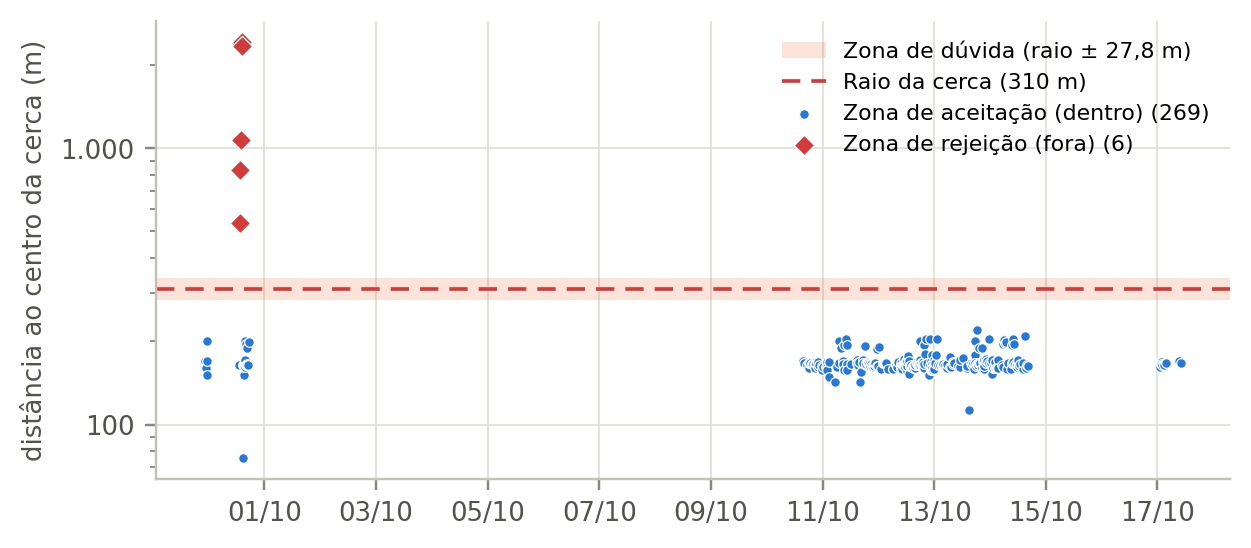
\includegraphics[width=\textwidth]{figuras/uc1_zonas.jpg}
  \fonte{Elaborado pelo autor (2026).}
\end{figure}

As 269 posições dentro da cerca ficaram a até 220 m do centro, na zona de aceitação. As seis posições de 30/09 ficaram a pelo menos 536 m, na zona de rejeição, e nenhuma posição caiu na zona de dúvida. O alerta de saída da cerca de 30/09 não depende, portanto, da incerteza da posição.

\subsection{Parâmetros calculados pelo site}

O site calcula, a partir das posições gravadas no banco, quatro parâmetros para o intervalo escolhido. A distância percorrida é a soma das distâncias entre posições consecutivas, $d = \sum_k s_k$. A velocidade média é essa distância dividida pelo tempo $T$ entre a primeira e a última posição. A velocidade máxima é a maior razão $s_k/\Delta t_k$ entre duas posições consecutivas. A aceleração média é a média das variações de velocidade entre trechos seguidos.

A incerteza desses resultados foi propagada pelo método da perturbação sequencial \cite{moffat1988}, aplicado à mesma função de cálculo do site. Cada entrada $X_i$ (latitude, longitude e horário de cada posição) foi aumentada e reduzida pela sua incerteza $\delta X_i$, uma de cada vez, e a contribuição $C_i$ foi tomada como a média de $|R_{i+} - R_0|$ e $|R_{i-} - R_0|$, porque o resultado não é linear nas posições. A incerteza do resultado é a soma quadrática das contribuições,
\begin{equation}
  \delta R = \sqrt{\sum_i C_i^2}, \qquad C_i \approx \frac{\partial R}{\partial X_i}\,\delta X_i,
  \label{eq:uc1-perturbacao}
\end{equation}
e tem o mesmo nível de confiança das entradas, 95\%. Para a velocidade média, a propagação analítica da apostila de \citeonline{poiate},
\begin{equation}
  \frac{\delta \bar v}{\bar v} = \sqrt{\left(\frac{\delta d}{d}\right)^2 + \left(\frac{\delta T}{T}\right)^2},
  \label{eq:uc1-vmed}
\end{equation}
com $\delta T = 1$~s (metade da resolução em cada extremo), deu o mesmo valor que a perturbação sequencial até a terceira casa. A parcela do horário foi desprezível em todos os resultados, exceto na velocidade máxima de 13/10, em que foi de 23 km/h contra 128 km/h da parcela das posições.

A soma de passos tem também um erro fixo, que \citeonline{moffat1988} classifica como erro conceitual: com a \textit{tag} parada, o ruído da posição gera passos de comprimento não nulo, e o site os soma como distância. Esse erro foi medido no experimento auxiliar, com 121 pares de leituras consecutivas sem leitura em comum. O passo médio foi de $(14{,}0 \pm 3{,}3)$~m, em que a incerteza é $t\,S/\sqrt{N}$, com $t = 1{,}98$ para 120 graus de liberdade. Para um intervalo com $k$ passos, o erro fixo é $B = k \times 14{,}0$~m, e a sua incerteza, $k \times 3{,}3$~m, somada de forma linear, porque o mesmo valor médio é usado em todos os passos. A distância corrigida é $d - B$, e a sua incerteza de ordem $N$ é a soma quadrática da incerteza propagada com a incerteza de $B$. Essa correção supõe a \textit{tag} parada em todos os passos e, nos dias com deslocamento, superestima o erro fixo. A velocidade média recebe a mesma correção, dividida por $T$.

A Figura~\ref{fig:uc1-parametros} apresenta, por dia, o valor calculado pelo site, a incerteza expandida e o erro fixo. Um valor foi considerado significativo quando superou a sua incerteza, isto é, quando a diferença em relação a zero (ou ao erro fixo, no caso da distância e da velocidade média) foi maior que a incerteza dessa diferença \cite{moffat1988}.

\begin{figure}[htb]
  \centering
  \caption{Parâmetros calculados pelo site por dia, com a incerteza expandida e o erro fixo}
  \label{fig:uc1-parametros}
  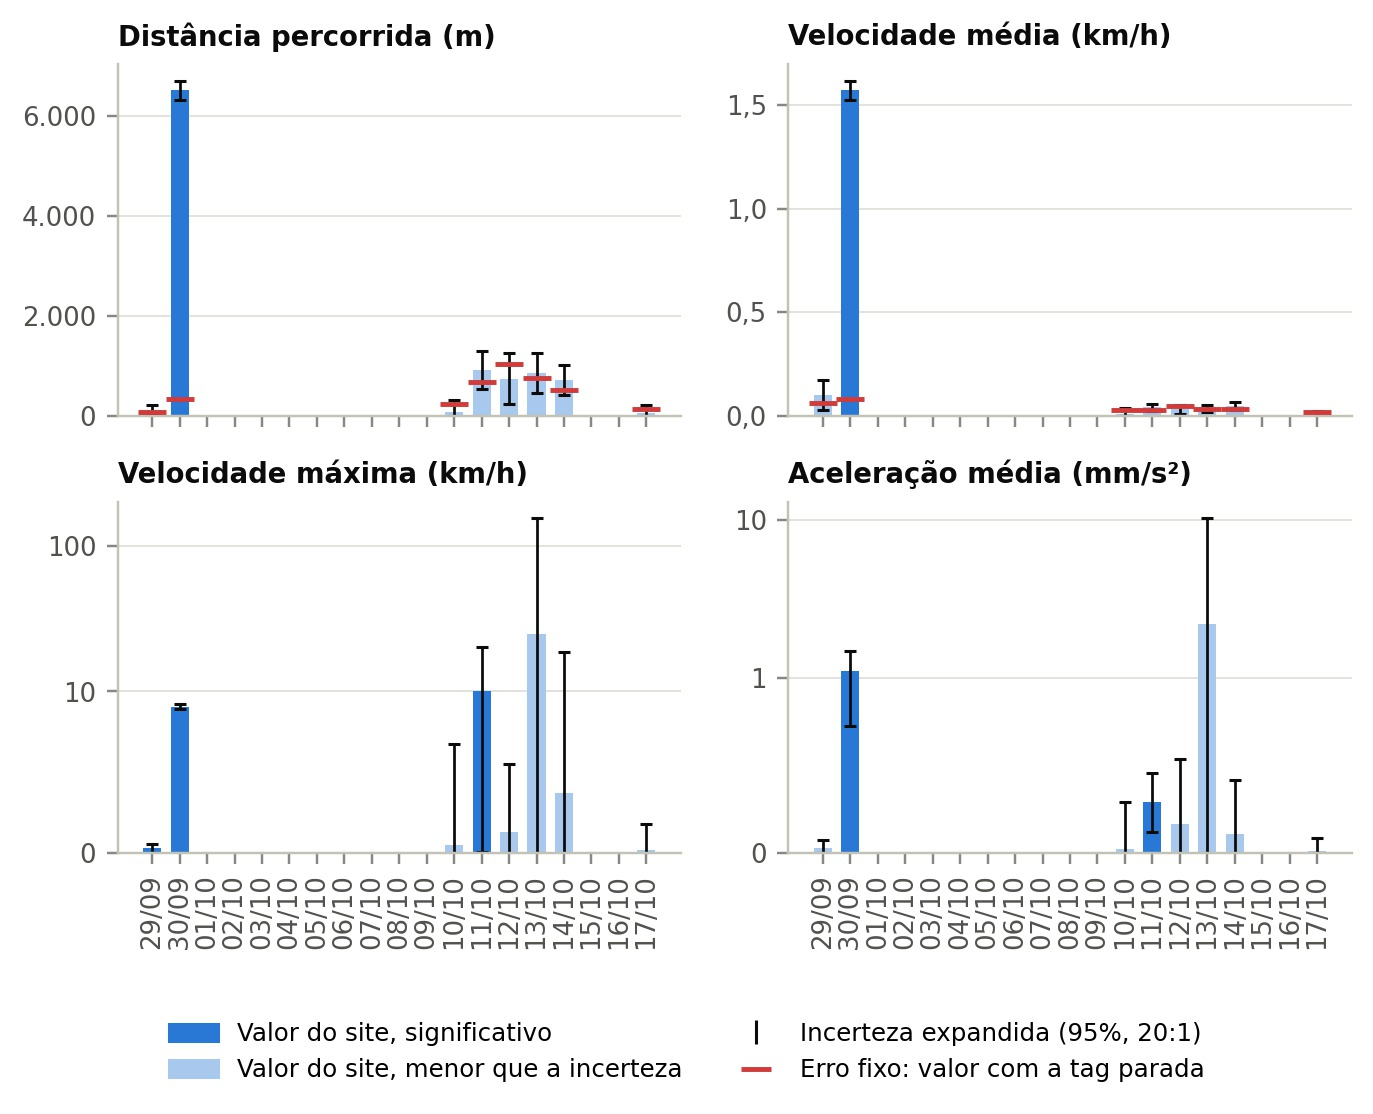
\includegraphics[width=\textwidth]{figuras/uc1_parametros.jpg}
  \fonte{Elaborado pelo autor (2026).}
\end{figure}

A Tabela~\ref{tab:uc1-dia30} reúne os resultados de 30/09, o dia com deslocamento, em 24 posições e 4 h 08 min. Todos os parâmetros foram significativos. A distância corrigida foi de $(6{,}19 \pm 0{,}19)$~km, com incerteza relativa de 3\%.

\begin{table}[htb]
  \centering
  \caption{Parâmetros de 30/09 a 95\% de confiança}
  \label{tab:uc1-dia30}
  \begin{tabular}{lrrr}
    \hline
    \textbf{Parâmetro} & \textbf{Valor do site} & \textbf{Erro fixo} & \textbf{Valor corrigido} \\
    \hline
    Distância percorrida & $(6{,}51 \pm 0{,}17)$ km & $(0{,}32 \pm 0{,}08)$ km & $(6{,}19 \pm 0{,}19)$ km \\
    Velocidade média & $(1{,}57 \pm 0{,}04)$ km/h & 0,08 km/h & $(1{,}50 \pm 0{,}05)$ km/h \\
    Velocidade máxima & $(9{,}0 \pm 0{,}2)$ km/h & --- & --- \\
    Aceleração média & $(1{,}1 \pm 0{,}4)$ mm/s² & --- & --- \\
    \hline
  \end{tabular}
  \fonte{Elaborado pelo autor (2026).}
\end{table}

Nos dias com a \textit{tag} parada, a distância corrigida foi compatível com zero. Em 11/10, por exemplo, o site somou 914 m, o erro fixo foi de 674 m e a distância corrigida, $(240 \pm 370)$~m. A velocidade máxima de 11/10, $(10 \pm 10)$~km/h, ficou no limite da significância, e a de 13/10, 24,7 km/h, teve incerteza de 130 km/h, porque vem de duas posições recebidas com poucos segundos de diferença. A Tabela~\ref{tab:uc1-total} reúne os parâmetros do intervalo total.

\begin{table}[htb]
  \centering
  \caption{Parâmetros calculados pelo site no intervalo total (29/09 a 17/10), a 95\% de confiança}
  \label{tab:uc1-total}
  \begin{tabular}{lrrr}
    \hline
    \textbf{Parâmetro} & \textbf{Valor do site} & \textbf{Erro fixo} & \textbf{Valor corrigido} \\
    \hline
    Distância percorrida & $(10{,}1 \pm 0{,}8)$ km & $(3{,}8 \pm 0{,}9)$ km & $(6{,}2 \pm 1{,}2)$ km \\
    Velocidade média & $(0{,}024 \pm 0{,}002)$ km/h & 0,009 km/h & $(0{,}015 \pm 0{,}003)$ km/h \\
    Velocidade máxima & $(25 \pm 130)$ km/h & --- & --- \\
    Aceleração média & $(0{,}7 \pm 1{,}7)$ mm/s² & --- & --- \\
    \hline
  \end{tabular}
  \fonte{Elaborado pelo autor (2026).}
\end{table}

A distância corrigida do intervalo total, $(6{,}2 \pm 1{,}2)$~km, coincide com a de 30/09: o restante dos 10,1 km somados pelo site corresponde ao ruído da posição nos dias parados. Um passo de comprimento próximo de zero tem incerteza de $\sqrt{2}\,\delta y = 39{,}5$~m, e 243 dos 274 passos do intervalo ficaram abaixo desse valor. A velocidade máxima e a aceleração média do intervalo total têm incerteza maior que o próprio valor e não permitem conclusões.

Com intervalos medianos de 16 min e incerteza de 19 m (leste) e 28 m (norte) a 95\% de confiança, a localização pela rede Find Hub atende à verificação da cerca virtual, sem posições na zona de dúvida. Para medir distância e velocidade em treinos, o cálculo do site precisaria descontar o erro fixo ou descartar passos menores que a incerteza de um passo, ou essas grandezas teriam de vir do acelerômetro.
. Figuras em figuras/*.jpg.
% Incerteza: Moffat (1988) e Poiate Junior (apostila), chaves em referencias.bib.
% Trechos marcados com "CONFERIR" dependem de informação do autor.
% =====================================================================

\section{Caso de uso 1: localização}
\label{sec:res-localizacao}

O intervalo analisado vai de 29/09/2026 a 17/10/2026 e reúne 275 posições da \textit{tag}. As 32 primeiras, até 10/10, foram coletadas pela instância local do servidor, antes da implantação; as 243 seguintes, pela instância em produção. As duas instâncias usam o mesmo código de consulta e de filtragem. Entre 30/09 e 10/10 não há posições, porque o servidor local ficou desligado nesse período. % CONFERIR: motivo da lacuna
As posições estão em metros a partir do centro da cerca virtual, sem mapa de fundo, para não expor o endereço do local de teste.

A Figura~\ref{fig:uc1-trajeto} apresenta as posições em duas escalas. Em (a), o período de 10/10 a 17/10, com a \textit{tag} parada dentro da cerca de 310 m de raio. Em (b), o intervalo total, que inclui o deslocamento a pé feito pelo autor em 30/09.

\begin{figure}[htb]
  \centering
  \caption{Posições recebidas da \textit{tag} e cerca virtual: (a) período com a \textit{tag} parada; (b) intervalo total}
  \label{fig:uc1-trajeto}
  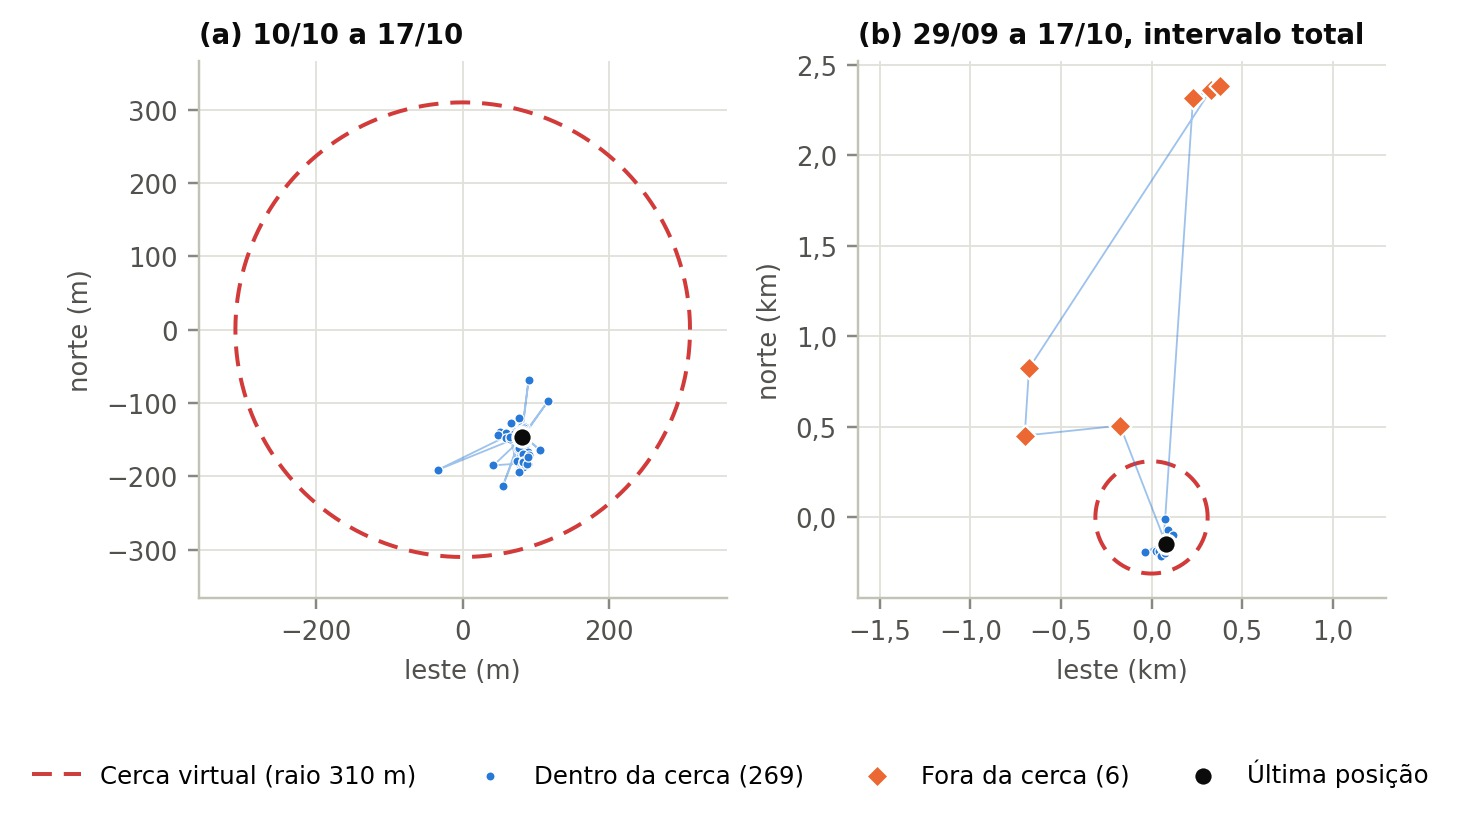
\includegraphics[width=\textwidth]{figuras/uc1_trajeto.jpg}
  \fonte{Elaborado pelo autor (2026).}
\end{figure}

Seis posições ficaram fora da cerca, todas em 30/09, entre 13h32 e 14h31, a até 2,41 km do centro. O site registrou o alerta de saída da cerca a partir da primeira delas: o cartão de localização do cavalo passou a indicar ``Fora da cerca'' e o alerta apareceu no sino do portal. Nas demais 269 posições a \textit{tag} estava dentro do raio.

A Figura~\ref{fig:uc1-dia} mostra quantas posições chegaram em cada dia. A quantidade variou de 6 a 75 por dia. A rede Find Hub depende de celulares Android que passem perto da \textit{tag}, e o servidor só registra o que a rede entrega.

\begin{figure}[htb]
  \centering
  \caption{Posições recebidas por dia, dentro e fora da cerca}
  \label{fig:uc1-dia}
  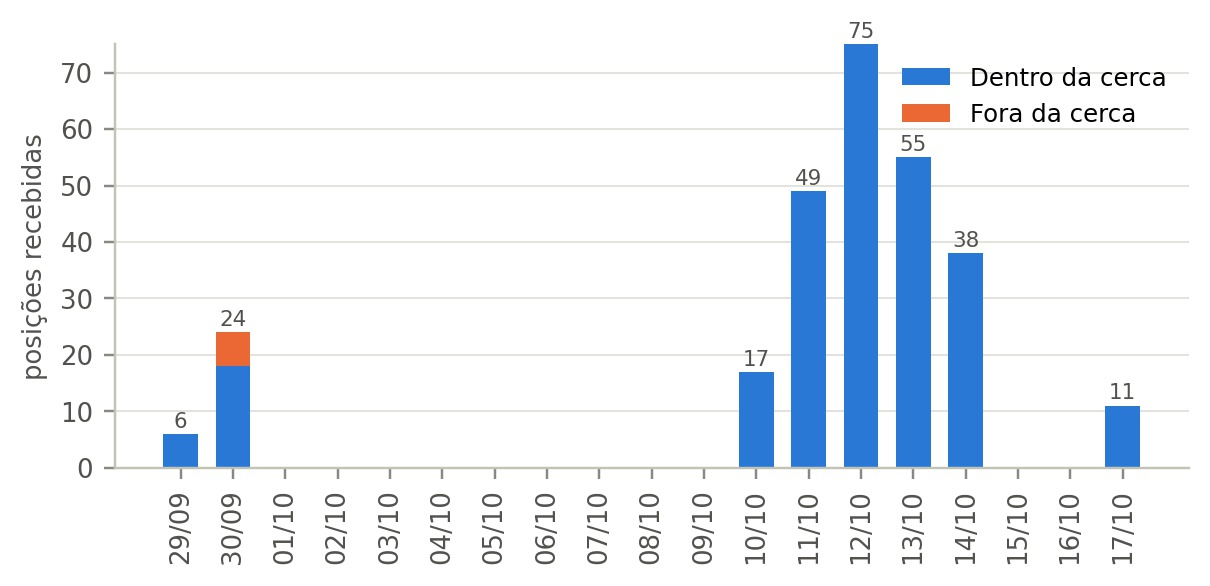
\includegraphics[width=\textwidth]{figuras/uc1_por_dia.jpg}
  \fonte{Elaborado pelo autor (2026).}
\end{figure}

A Figura~\ref{fig:uc1-intervalo} apresenta o intervalo entre posições consecutivas e a precisão informada pela rede em cada posição. O intervalo mediano foi de 16 min, e 90\% dos intervalos ficaram abaixo de 57 min; o maior intervalo, de 239 h, corresponde à lacuna entre 30/09 e 10/10. A precisão informada teve mediana de 75 m, e 46\% das posições chegaram com o valor máximo aceito pelo filtro do servidor, 100 m.

\begin{figure}[htb]
  \centering
  \caption{Intervalo entre posições consecutivas e precisão informada pela rede}
  \label{fig:uc1-intervalo}
  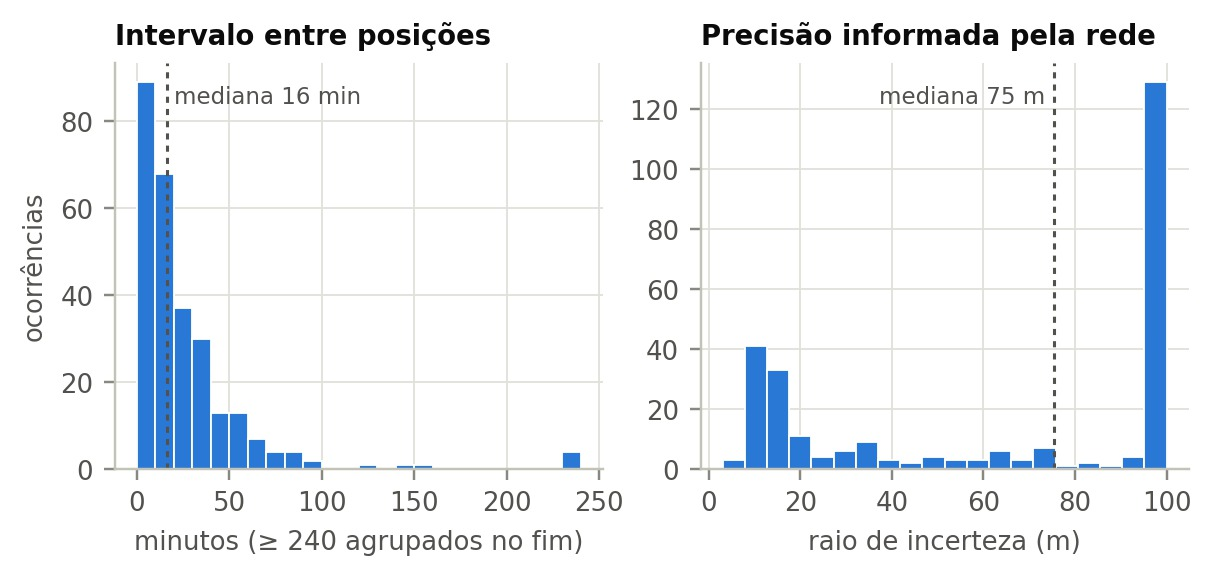
\includegraphics[width=\textwidth]{figuras/uc1_intervalo_precisao.jpg}
  \fonte{Elaborado pelo autor (2026).}
\end{figure}

\subsection{Incerteza da posição}
\label{sec:uc1-incerteza-posicao}

A incerteza foi avaliada pela análise de amostra única de \citeonline{moffat1988}: cada posição é uma leitura isolada, e a dispersão do sistema de medição é obtida de um experimento auxiliar feito em condição representativa. O experimento auxiliar foi o período de 10/10 a 17/10, com a \textit{tag} parada no mesmo ponto e 243 leituras. As coordenadas foram convertidas para metros nas direções leste ($x$) e norte ($y$), e o desvio-padrão amostral de cada direção foi $S_x = 9{,}6$~m e $S_y = 14{,}0$~m.

Com 242 graus de liberdade, a distribuição qui-quadrado limita o desvio-padrão da população a $0{,}92\,S \le \sigma \le 1{,}10\,S$, ao nível de 95\% \cite{moffat1988}. Foi adotado o valor mais provável, $\sigma = S$. A incerteza de uma leitura isolada, a 95\% de confiança (chance de 20 para 1), é
\begin{equation}
  \delta x = 2\sigma_x = 19{,}2~\text{m}, \qquad \delta y = 2\sigma_y = 27{,}9~\text{m}.
  \label{eq:uc1-incerteza-posicao}
\end{equation}
Com o limite superior de $\sigma$, os valores seriam 21,0 m e 30,6 m. Nos dados, 96,3\% das leituras ficaram dentro de $\pm\delta x$ e 92,2\% dentro de $\pm\delta y$. A distribuição não é gaussiana, pois 92\% das leituras na direção leste ficaram dentro de $\pm S_x$, e uma leitura isolada se afastou 121 m da média. A autocorrelação entre leituras consecutivas foi de $-0{,}001$ (leste) e $0{,}12$ (norte), e as leituras foram tratadas como independentes, condição exigida para a soma quadrática.

A Tabela~\ref{tab:uc1-ordens} separa a incerteza da posição nas três ordens de \citeonline{moffat1988}. A ordem zero corresponde à resolução dos valores recebidos, que chegam com $10^{-7}$ grau (cerca de 1,1 cm), e a incerteza instrumental é a metade da resolução \cite{poiate}. O horário de cada posição chega em segundos inteiros, com incerteza de 0,5 s. A primeira ordem é a dispersão medida no experimento auxiliar. Na ordem $N$ entraria o erro fixo da rede, isto é, a diferença entre a média das leituras e a posição verdadeira da \textit{tag}. Esse erro não foi medido, porque não havia uma referência de posição com incerteza menor; ele desloca todas as leituras da mesma forma, e por isso se cancela nas diferenças entre posições usadas na distância e na velocidade, mas afeta a verificação da cerca.

\begin{table}[htb]
  \centering
  \caption{Incerteza de uma posição a 95\% de confiança}
  \label{tab:uc1-ordens}
  \begin{tabular}{lrrl}
    \hline
    \textbf{Ordem} & \textbf{Leste (m)} & \textbf{Norte (m)} & \textbf{Origem} \\
    \hline
    Zero & 0,005 & 0,006 & resolução de $10^{-7}$ grau \\
    Primeira & 19,2 & 27,9 & experimento auxiliar, $2S$ \\
    $N$ & 19,2 & 27,9 & erro fixo da rede não avaliado \\
    \hline
  \end{tabular}
  \fonte{Elaborado pelo autor (2026).}
\end{table}

A ordem zero é cerca de 4 mil vezes menor que a primeira e foi desprezada, pois uma parcela menor que um terço da maior tem efeito pequeno na soma quadrática \cite{moffat1988}. Em 95,9\% das leituras paradas, a distância até a média ficou abaixo da precisão informada pela rede para aquela leitura, cuja mediana foi de 75 m. A precisão informada se comporta como um limite conservador, maior que a incerteza medida.

\subsection{Verificação da cerca com a incerteza}

A cerca virtual funciona como uma tolerância: a posição é aceita enquanto a distância $r$ até o centro não passa do raio $R = 310$~m. Seguindo \citeonline{poiate}, a incerteza de medição divide a faixa em três zonas. A zona de aceitação vai até $R - \delta r$, a zona de rejeição começa em $R + \delta r$ e, entre as duas, fica a zona de dúvida, onde a medição não permite afirmar se a \textit{tag} está dentro ou fora. A incerteza da distância ao centro vem da propagação das incertezas da Equação~\eqref{eq:uc1-incerteza-posicao}:
\begin{equation}
  \delta r = \sqrt{\left(\frac{x}{r}\,\delta x\right)^2 + \left(\frac{y}{r}\,\delta y\right)^2}.
  \label{eq:uc1-incerteza-raio}
\end{equation}

O maior valor de $\delta r$ entre as posições foi de 27,8 m, o que coloca a zona de dúvida entre 282 m e 338 m. A incerteza ficou abaixo de um décimo do intervalo de tolerância (31 m), critério de equilíbrio entre custo e qualidade recomendado por \citeonline{poiate}. A Figura~\ref{fig:uc1-zonas} mostra a distância de cada posição ao centro com as três zonas.

\begin{figure}[htb]
  \centering
  \caption{Distância das posições ao centro da cerca, com as zonas de aceitação, dúvida e rejeição}
  \label{fig:uc1-zonas}
  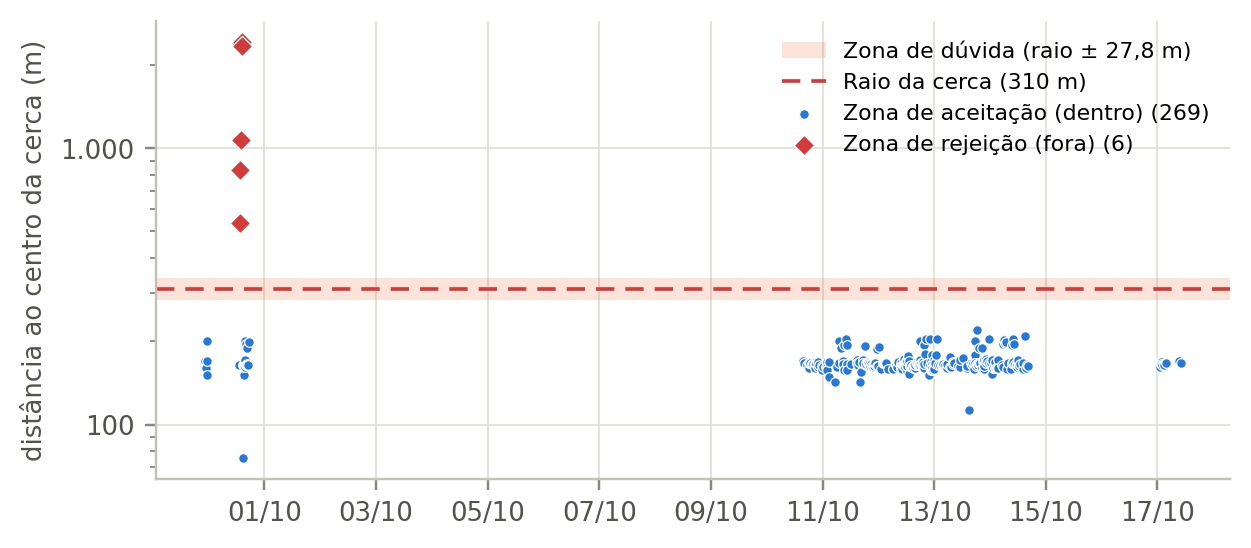
\includegraphics[width=\textwidth]{figuras/uc1_zonas.jpg}
  \fonte{Elaborado pelo autor (2026).}
\end{figure}

As 269 posições dentro da cerca ficaram a até 220 m do centro, na zona de aceitação. As seis posições de 30/09 ficaram a pelo menos 536 m, na zona de rejeição, e nenhuma posição caiu na zona de dúvida. O alerta de saída da cerca de 30/09 não depende, portanto, da incerteza da posição.

\subsection{Parâmetros calculados pelo site}

O site calcula, a partir das posições gravadas no banco, quatro parâmetros para o intervalo escolhido. A distância percorrida é a soma das distâncias entre posições consecutivas, $d = \sum_k s_k$. A velocidade média é essa distância dividida pelo tempo $T$ entre a primeira e a última posição. A velocidade máxima é a maior razão $s_k/\Delta t_k$ entre duas posições consecutivas. A aceleração média é a média das variações de velocidade entre trechos seguidos.

A incerteza desses resultados foi propagada pelo método da perturbação sequencial \cite{moffat1988}, aplicado à mesma função de cálculo do site. Cada entrada $X_i$ (latitude, longitude e horário de cada posição) foi aumentada e reduzida pela sua incerteza $\delta X_i$, uma de cada vez, e a contribuição $C_i$ foi tomada como a média de $|R_{i+} - R_0|$ e $|R_{i-} - R_0|$, porque o resultado não é linear nas posições. A incerteza do resultado é a soma quadrática das contribuições,
\begin{equation}
  \delta R = \sqrt{\sum_i C_i^2}, \qquad C_i \approx \frac{\partial R}{\partial X_i}\,\delta X_i,
  \label{eq:uc1-perturbacao}
\end{equation}
e tem o mesmo nível de confiança das entradas, 95\%. Para a velocidade média, a propagação analítica da apostila de \citeonline{poiate},
\begin{equation}
  \frac{\delta \bar v}{\bar v} = \sqrt{\left(\frac{\delta d}{d}\right)^2 + \left(\frac{\delta T}{T}\right)^2},
  \label{eq:uc1-vmed}
\end{equation}
com $\delta T = 1$~s (metade da resolução em cada extremo), deu o mesmo valor que a perturbação sequencial até a terceira casa. A parcela do horário foi desprezível em todos os resultados, exceto na velocidade máxima de 13/10, em que foi de 23 km/h contra 128 km/h da parcela das posições.

A soma de passos tem também um erro fixo, que \citeonline{moffat1988} classifica como erro conceitual: com a \textit{tag} parada, o ruído da posição gera passos de comprimento não nulo, e o site os soma como distância. Esse erro foi medido no experimento auxiliar, com 121 pares de leituras consecutivas sem leitura em comum. O passo médio foi de $(14{,}0 \pm 3{,}3)$~m, em que a incerteza é $t\,S/\sqrt{N}$, com $t = 1{,}98$ para 120 graus de liberdade. Para um intervalo com $k$ passos, o erro fixo é $B = k \times 14{,}0$~m, e a sua incerteza, $k \times 3{,}3$~m, somada de forma linear, porque o mesmo valor médio é usado em todos os passos. A distância corrigida é $d - B$, e a sua incerteza de ordem $N$ é a soma quadrática da incerteza propagada com a incerteza de $B$. Essa correção supõe a \textit{tag} parada em todos os passos e, nos dias com deslocamento, superestima o erro fixo. A velocidade média recebe a mesma correção, dividida por $T$.

A Figura~\ref{fig:uc1-parametros} apresenta, por dia, o valor calculado pelo site, a incerteza expandida e o erro fixo. Um valor foi considerado significativo quando superou a sua incerteza, isto é, quando a diferença em relação a zero (ou ao erro fixo, no caso da distância e da velocidade média) foi maior que a incerteza dessa diferença \cite{moffat1988}.

\begin{figure}[htb]
  \centering
  \caption{Parâmetros calculados pelo site por dia, com a incerteza expandida e o erro fixo}
  \label{fig:uc1-parametros}
  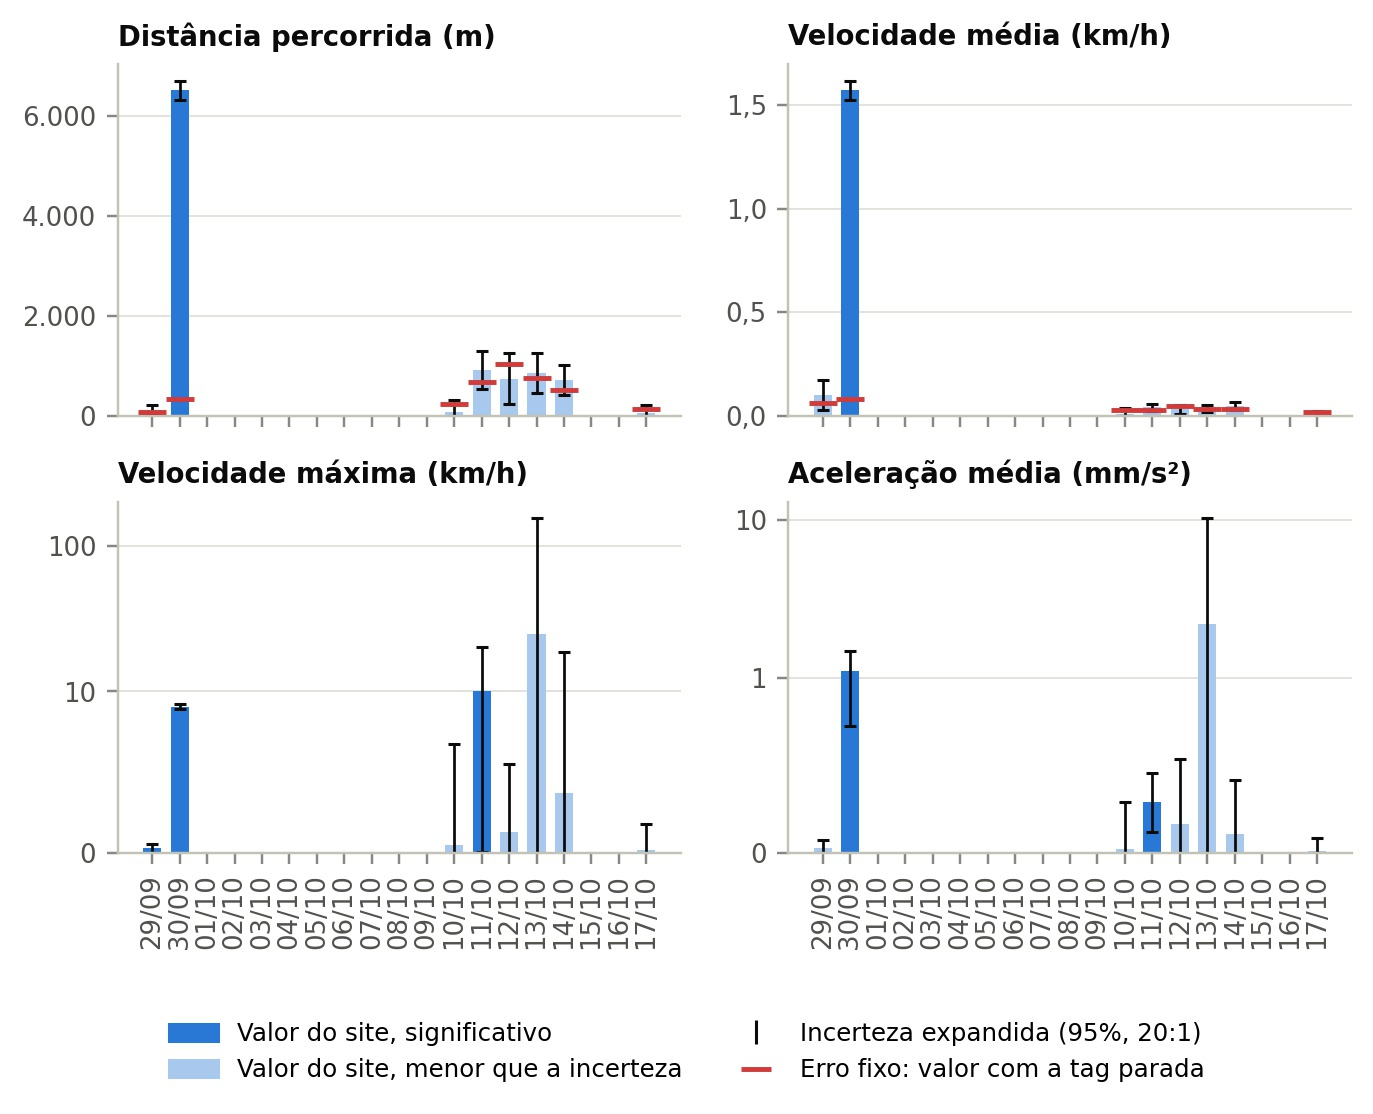
\includegraphics[width=\textwidth]{figuras/uc1_parametros.jpg}
  \fonte{Elaborado pelo autor (2026).}
\end{figure}

A Tabela~\ref{tab:uc1-dia30} reúne os resultados de 30/09, o dia com deslocamento, em 24 posições e 4 h 08 min. Todos os parâmetros foram significativos. A distância corrigida foi de $(6{,}19 \pm 0{,}19)$~km, com incerteza relativa de 3\%.

\begin{table}[htb]
  \centering
  \caption{Parâmetros de 30/09 a 95\% de confiança}
  \label{tab:uc1-dia30}
  \begin{tabular}{lrrr}
    \hline
    \textbf{Parâmetro} & \textbf{Valor do site} & \textbf{Erro fixo} & \textbf{Valor corrigido} \\
    \hline
    Distância percorrida & $(6{,}51 \pm 0{,}17)$ km & $(0{,}32 \pm 0{,}08)$ km & $(6{,}19 \pm 0{,}19)$ km \\
    Velocidade média & $(1{,}57 \pm 0{,}04)$ km/h & 0,08 km/h & $(1{,}50 \pm 0{,}05)$ km/h \\
    Velocidade máxima & $(9{,}0 \pm 0{,}2)$ km/h & --- & --- \\
    Aceleração média & $(1{,}1 \pm 0{,}4)$ mm/s² & --- & --- \\
    \hline
  \end{tabular}
  \fonte{Elaborado pelo autor (2026).}
\end{table}

Nos dias com a \textit{tag} parada, a distância corrigida foi compatível com zero. Em 11/10, por exemplo, o site somou 914 m, o erro fixo foi de 674 m e a distância corrigida, $(240 \pm 370)$~m. A velocidade máxima de 11/10, $(10 \pm 10)$~km/h, ficou no limite da significância, e a de 13/10, 24,7 km/h, teve incerteza de 130 km/h, porque vem de duas posições recebidas com poucos segundos de diferença. A Tabela~\ref{tab:uc1-total} reúne os parâmetros do intervalo total.

\begin{table}[htb]
  \centering
  \caption{Parâmetros calculados pelo site no intervalo total (29/09 a 17/10), a 95\% de confiança}
  \label{tab:uc1-total}
  \begin{tabular}{lrrr}
    \hline
    \textbf{Parâmetro} & \textbf{Valor do site} & \textbf{Erro fixo} & \textbf{Valor corrigido} \\
    \hline
    Distância percorrida & $(10{,}1 \pm 0{,}8)$ km & $(3{,}8 \pm 0{,}9)$ km & $(6{,}2 \pm 1{,}2)$ km \\
    Velocidade média & $(0{,}024 \pm 0{,}002)$ km/h & 0,009 km/h & $(0{,}015 \pm 0{,}003)$ km/h \\
    Velocidade máxima & $(25 \pm 130)$ km/h & --- & --- \\
    Aceleração média & $(0{,}7 \pm 1{,}7)$ mm/s² & --- & --- \\
    \hline
  \end{tabular}
  \fonte{Elaborado pelo autor (2026).}
\end{table}

A distância corrigida do intervalo total, $(6{,}2 \pm 1{,}2)$~km, coincide com a de 30/09: o restante dos 10,1 km somados pelo site corresponde ao ruído da posição nos dias parados. Um passo de comprimento próximo de zero tem incerteza de $\sqrt{2}\,\delta y = 39{,}5$~m, e 243 dos 274 passos do intervalo ficaram abaixo desse valor. A velocidade máxima e a aceleração média do intervalo total têm incerteza maior que o próprio valor e não permitem conclusões.

Com intervalos medianos de 16 min e incerteza de 19 m (leste) e 28 m (norte) a 95\% de confiança, a localização pela rede Find Hub atende à verificação da cerca virtual, sem posições na zona de dúvida. Para medir distância e velocidade em treinos, o cálculo do site precisaria descontar o erro fixo ou descartar passos menores que a incerteza de um passo, ou essas grandezas teriam de vir do acelerômetro.


% ---------------------------------------------------------------------
\section{Caso de uso 2: coleta biométrica}
\label{sec:res-biometria}

A Figura~\ref{fig:uc2-cobertura} mostra, para cada dia com o sensor ligado, quantos minutos têm leitura de cada sinal no servidor. O movimento somou 959 min e a temperatura 785 min. As leituras de frequência cardíaca somaram 304 s, distribuídos em oito janelas.

\begin{figure}[htb]
  \centering
  \caption{Minutos com leitura no servidor, por dia e por sinal}
  \label{fig:uc2-cobertura}
  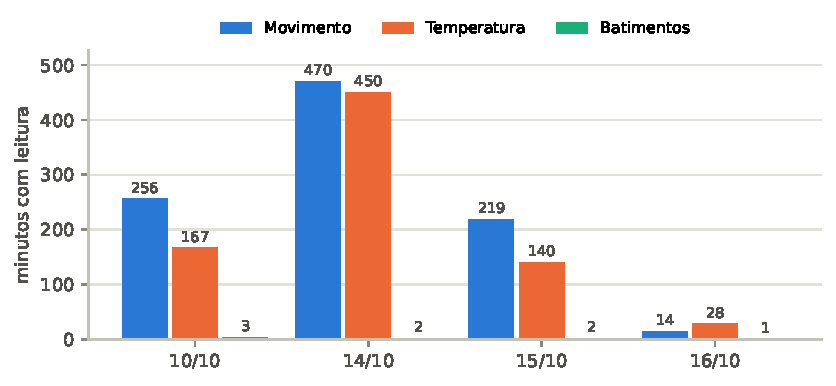
\includegraphics[width=0.95\linewidth]{figures/uc2_cobertura.pdf}
  \fonte{Elaborado pelo autor (2026).}
\end{figure}

A incerteza de cada sinal seguiu o mesmo procedimento do caso de uso 1 \cite{moffat1988}. A ordem zero é a metade da resolução do valor recebido \cite{poiate}; a primeira ordem é $2S$, com $S$ medido em um experimento auxiliar com o sensor em condição estável; o erro fixo vem da folha de dados ou de uma medição com valor conhecido; e a ordem $N$ é a soma quadrática dessas parcelas, a 95\% de confiança. A Tabela~\ref{tab:uc2-incerteza} resume os valores.

\begin{table}[htb]
  \centering
  \caption{Incerteza dos sinais biométricos a 95\% de confiança}
  \label{tab:uc2-incerteza}
  \begin{tabular}{lrrrr}
    \hline
    \textbf{Sinal} & \textbf{Ordem zero} & \textbf{1.ª ordem} & \textbf{Erro fixo} & \textbf{Ordem $N$} \\
    \hline
    Temperatura & 0,05 °C & 0,6 °C & 2,0 °C & 2,1 °C \\
    Movimento (minuto) & 0,00003 $g$ & 0,003 $g$ & 0,076 $g$ & 0,003 $g$\textsuperscript{a} \\
    Um batimento & 3,5 bpm & 6,0 bpm & não avaliado & 6,0 bpm \\
    Média de 16/10 & --- & 0,7 bpm & não avaliado & 0,7 bpm \\
    \hline
  \end{tabular}
  \fonte{Elaborado pelo autor (2026). \textsuperscript{a}Após descontar o erro fixo.}
\end{table}

\subsection{Frequência cardíaca}

O MAX30102 só calcula batimentos com pele encostada no sensor, e nos ensaios ele foi usado com o dedo do autor por poucos segundos. % CONFERIR
A Tabela~\ref{tab:bpm} lista as oito janelas. O sensor lê 25 vezes por segundo, e o intervalo entre dois picos tem resolução de 1/25 s. Pela propagação de $f = 60/T$, uma resolução $\delta T$ no período gera $\delta f = 60\,\delta T/T^2$ na frequência \cite{poiate}, valor que cresce com o quadrado da frequência: 3,5 bpm a 72 bpm e 21 bpm a 177 bpm.
% PROVISÓRIO: a janela de 16/10 00:03 tem valores fictícios (uc2.py, JANELA_PROVISORIA). Substituir pela medição real antes da entrega.

\begin{table}[htb]
  \centering
  \caption{Janelas com leitura de frequência cardíaca (bpm)}
  \label{tab:bpm}
  \begin{tabular}{lrrrrr}
    \hline
    \textbf{Início} & \textbf{Duração (s)} & \textbf{Média} & \textbf{Mínimo} & \textbf{Máximo} & \textbf{Resolução} \\
    \hline
    10/10 19:27 & 31 & 60,2 & 28,1 & 106,8 & 2,4 \\
    10/10 19:27 & 9 & 51,0 & 27,1 & 76,3 & 1,7 \\
    10/10 19:28 & 57 & 62,4 & 34,1 & 79,7 & 2,6 \\
    14/10 18:07 & 29 & 62,7 & 23,0 & 75,7 & 2,6 \\
    14/10 21:12 & 55 & 53,6 & 21,7 & 105,3 & 1,9 \\
    15/10 20:34 & 8 & 78,5 & 34,2 & 177,0 & 4,1 \\
    15/10 23:54 & 55 & 67,0 & 31,0 & 176,5 & 3,0 \\
    16/10 00:03 & 60 & 72,5 & 68,2 & 78,9 & 3,5 \\ % PROVISÓRIO
    \hline
  \end{tabular}
  \fonte{Elaborado pelo autor (2026). Resolução de um batimento na frequência média da janela.}
\end{table}

Nas sete primeiras janelas, os mínimos (22 a 34 bpm) e os máximos (até 177 bpm) se afastam da média muito mais que a resolução, o que mostra que o algoritmo de detecção de pulso aceitou picos falsos quando o dedo se moveu. O sensor dividia o barramento I2C com o MPU6050 em fios sem solda, e as falhas de contato desligaram a leitura de batimentos em parte do período. Na janela de 16/10, com 60 s de contato contínuo, a Figura~\ref{fig:uc2-batimentos} mostra os 73 batimentos. A média foi de $(72{,}5 \pm 0{,}7)$~bpm, com $S = 3{,}0$~bpm e $t = 1{,}99$ para 72 graus de liberdade, e a incerteza de um batimento isolado foi de $\pm 6{,}0$~bpm. Os valores se repetem em 68,2, 71,4, 75,0 e 78,9 bpm porque o período é contado em passos de 40 ms, e a resolução responde por boa parte da dispersão. O erro fixo do sensor exige comparação com um oxímetro de referência e não foi avaliado. % CONFERIR

\begin{figure}[htb]
  \centering
  \caption{Frequência de cada batimento na janela de 16/10, com a incerteza da média e de um batimento}
  \label{fig:uc2-batimentos}
  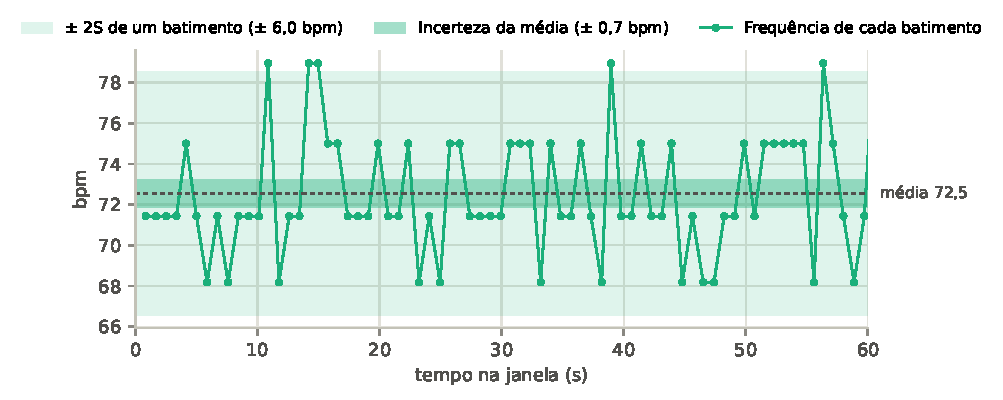
\includegraphics[width=0.95\linewidth]{figures/uc2_batimentos.pdf}
  \fonte{Elaborado pelo autor (2026).}
\end{figure}

\subsection{Temperatura}

A Figura~\ref{fig:uc2-temperatura} apresenta a temperatura como o portal a exibe, com a faixa de incerteza e os limites de alerta (35~°C e 40~°C) em vermelho. No dia 14/10 o DHT11 mediu o ar da sala, entre 24,0~°C e 27,9~°C em 450 leituras. A primeira ordem foi obtida das diferenças entre leituras sucessivas desse dia, que retiram a variação lenta da sala: $S = 0{,}30$~°C. A folha de dados do DHT11 informa exatidão de $\pm 2$~°C, adotada como erro fixo a 95\%. A ordem $N$ ficou em 2,1~°C, dominada pelo erro fixo.

\begin{figure}[htb]
  \centering
  \caption{Temperatura medida, incerteza e limites de alerta com as zonas de dúvida}
  \label{fig:uc2-temperatura}
  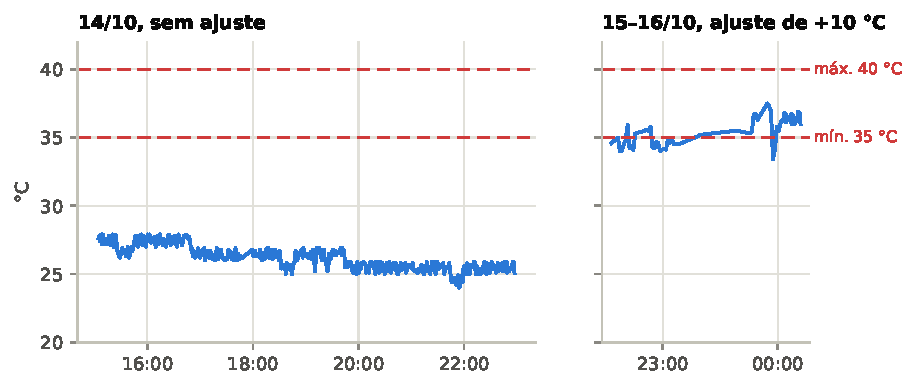
\includegraphics[width=0.95\linewidth]{figures/uc2_temperatura.pdf}
  \fonte{Elaborado pelo autor (2026).}
\end{figure}

Os limites de alerta formam uma tolerância de 5~°C. Pelo critério de \citeonline{poiate}, a incerteza deveria ficar abaixo de um décimo desse intervalo, 0,5~°C, e a do DHT11 é quatro vezes maior. A zona de aceitação fica reduzida a 37,1~°C a 37,9~°C, e as faixas de 32,9~°C a 37,1~°C e de 37,9~°C a 42,1~°C são zonas de dúvida, em que a medição não permite afirmar se a temperatura está dentro ou fora dos limites. As 450 leituras de 14/10 ficaram na zona de rejeição, abaixo do mínimo. Na noite de 15/10 foi salvo no portal um ajuste de +10~°C, usado para testar o caminho da calibração e não como correção medida. % CONFERIR
O sensor baixou o ajuste no envio seguinte e, a partir das 23h, as leituras passaram para a faixa de 33,4~°C a 37,5~°C: 47 das 49 leituras caíram na zona de dúvida e duas na zona de aceitação.

O teste confirma que o ajuste feito no portal chega ao sensor sem regravar o \textit{firmware} e passa a valer na comparação com os limites. O valor de +10~°C, porém, não corresponde a nenhuma referência e não reduz a incerteza: para uso no animal, o ajuste deve ser obtido comparando o sensor com um termômetro clínico, e um sensor com exatidão de 0,5~°C ou melhor atenderia ao critério de um décimo da tolerância.

\subsection{Movimento}

A Figura~\ref{fig:uc2-movimento} mostra a intensidade do movimento em 14/10, calculada como o afastamento do módulo da aceleração em relação a 1~$g$. Não havia limite de movimento configurado nesse dia. Nos 348 minutos com o sensor parado, a média por minuto foi de $(0{,}0761 \pm 0{,}0002)$~$g$, quando o esperado seria zero, com $S = 0{,}0016$~$g$ entre minutos. Nos 60 s mais estáveis das leituras brutas de 15/10, a 50 leituras/s, o módulo médio foi de 1,077~$g$, com $S = 0{,}003$~$g$ por leitura. O desvio de 0,076~$g$ é um erro fixo de escala do MPU6050, de 7,7\%, e é o motivo de o portal oferecer o ganho de calibração do movimento: com o ganho de $1/1{,}077$, a incerteza restante por minuto cai para 0,003~$g$. Sem a correção, o erro fixo precisa entrar na incerteza \cite{moffat1988}, e valores abaixo de cerca de 0,08~$g$ não se distinguem do sensor parado. Os picos de até 2,36~$g$ correspondem aos momentos em que o sensor foi manuseado e superam essa faixa com folga.

\begin{figure}[htb]
  \centering
  \caption{Intensidade do movimento por minuto em 14/10, com o erro fixo medido com o sensor parado (escala logarítmica acima de 0,1~$g$)}
  \label{fig:uc2-movimento}
  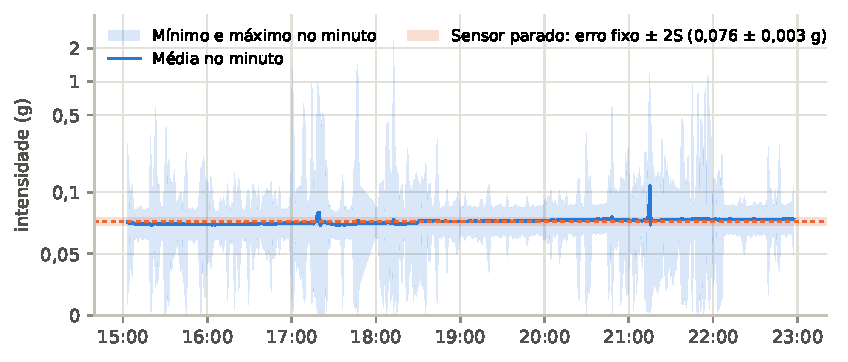
\includegraphics[width=0.95\linewidth]{figures/uc2_movimento.pdf}
  \fonte{Elaborado pelo autor (2026).}
\end{figure}

O envio de alertas por e-mail ao veterinário não foi avaliado, pois o servidor de e-mail (SMTP) não estava configurado no período. Os alertas pelo LED do sensor e pelo sino do portal foram verificados de forma visual, sem registro quantitativo. % CONFERIR

% ---------------------------------------------------------------------
\section{Caso de uso 3: detecção de padrões repetitivos}
\label{sec:res-padroes}

Os padrões ``Pulo'' e ``Volta'' foram avaliados em uma sessão de testes em 15/10, com 87,7 min de leituras do acelerômetro (263.089 amostras a 50 Hz). Nessa sessão o autor marcou no portal dez trechos, oito de Pulo e dois de Volta, que somam 22 s. Duas versões de detecção rodaram no sensor: até as 23h05, o modelo supervisionado treinado no servidor (floresta de 15 árvores de profundidade 4); depois desse horário, o detector físico descrito na metodologia.

A Figura~\ref{fig:uc3-sinal} mostra um trecho de 35 s com os três eixos, a marcação feita no portal (faixa cinza) e os eventos que o sensor registrou com o modelo supervisionado (linhas tracejadas).

\begin{figure}[htb]
  \centering
  \caption{Sinal do acelerômetro, trecho marcado como Pulo e eventos registrados pelo sensor}
  \label{fig:uc3-sinal}
  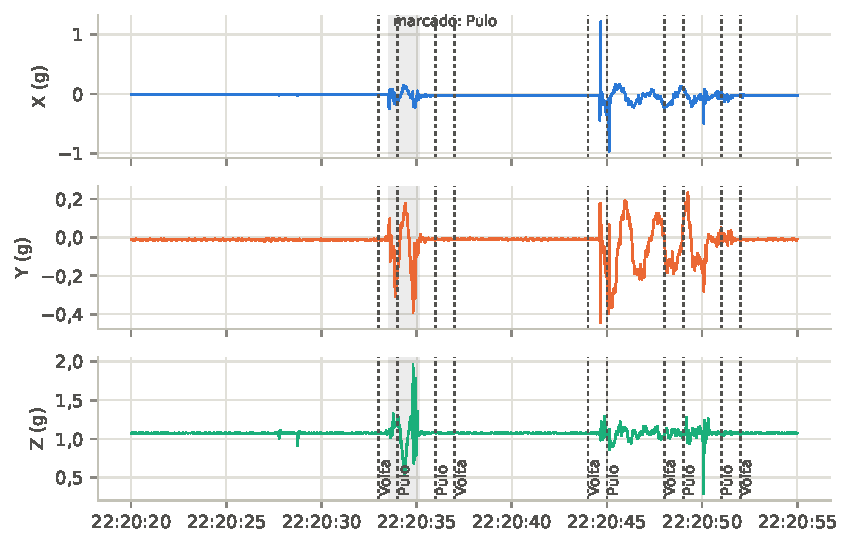
\includegraphics[width=0.95\linewidth]{figures/uc3_sinal_marcacoes.pdf}
  \fonte{Elaborado pelo autor (2026).}
\end{figure}

No trecho marcado, o eixo Z cai até cerca de 0,6~$g$ e sobe a quase 2~$g$, e o sensor registrou um Pulo dentro da marcação. O modelo, porém, também registrou eventos de Volta no mesmo instante e Pulos durante o manuseio seguinte, que não foi marcado. A Figura~\ref{fig:uc3-modelo} apresenta o desempenho do modelo supervisionado na validação feita pelo servidor no treino, deixando uma marcação de fora de cada vez.

\begin{figure}[htb]
  \centering
  \caption{Desempenho do modelo supervisionado na validação do treino}
  \label{fig:uc3-modelo}
  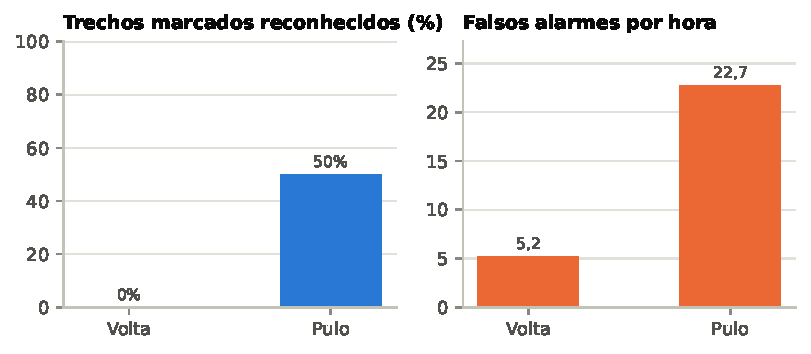
\includegraphics[width=0.95\linewidth]{figures/uc3_modelo_supervisionado.pdf}
  \fonte{Elaborado pelo autor (2026).}
\end{figure}

O modelo reconheceu 50\% dos trechos de Pulo, com 22,7 falsos alarmes por hora fora das marcações, e nenhum trecho de Volta. Com oito exemplos de Pulo (31 janelas) contra 3.000 janelas negativas, e dois exemplos de Volta, a base de treino é pequena demais para separar os padrões do manuseio comum do sensor. Esse resultado levou à troca do modelo supervisionado por um detector baseado na física do movimento, que não depende de exemplos marcados.

No detector físico, um salto é identificado pelo tempo $T$ em queda livre, em que o módulo da aceleração fica abaixo de 0,6~$g$. A altura vem da equação do lançamento vertical, $h = gT^2/8$, e o salto só é contado acima de 5~cm. A Figura~\ref{fig:uc3-voo} mostra os 20 voos com pelo menos 0,06 s encontrados ao reaplicar essa regra às leituras da sessão.

\begin{figure}[htb]
  \centering
  \caption{Altura estimada de cada voo pelo tempo em queda livre e limiar de contagem}
  \label{fig:uc3-voo}
  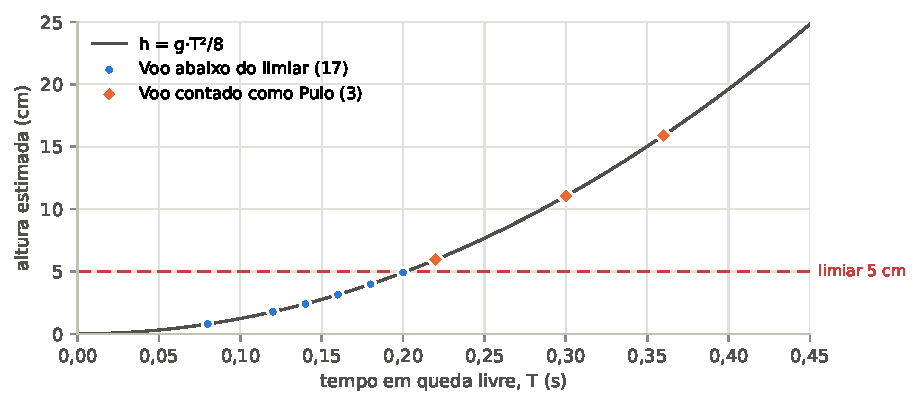
\includegraphics[width=0.95\linewidth]{figures/uc3_voo_altura.pdf}
  \fonte{Elaborado pelo autor (2026).}
\end{figure}

Três voos passaram do limiar, com 5,9 cm, 11 cm e 15,9 cm; os outros 17 ficaram entre 0,8 cm e 4,9 cm. Os oito trechos marcados como Pulo tiveram voos abaixo de 5 cm, de modo que nenhum deles foi contado. Os saltos do teste foram pequenos, feitos levantando e soltando a placa, e ficaram na faixa em que a regra não distingue um salto de um solavanco. Em um cavalo, um salto de 1 m corresponde a cerca de 0,9 s em queda livre, valor muito acima do ruído observado.

A Tabela~\ref{tab:uc3} compara as duas versões. A versão supervisionada é a que rodou no sensor até as 23h05; a física foi reaplicada às leituras da sessão inteira. Os eventos fora das marcações não equivalem a falsos alarmes, pois o autor não marcou todos os movimentos feitos durante a sessão.

\begin{table}[htb]
  \centering
  \caption{Marcações reconhecidas e eventos por versão de detecção na sessão de 15/10}
  \label{tab:uc3}
  \begin{tabular}{llrrr}
    \hline
    \textbf{Padrão} & \textbf{Versão} & \textbf{Marcações} & \textbf{Reconhecidas} & \textbf{Eventos} \\
    \hline
    Pulo  & Supervisionada (sensor) & 6 & 1 & 39 \\
    Volta & Supervisionada (sensor) & 2 & 0 & 42 \\
    Pulo  & Física (reaplicada) & 8 & 0 & 3 \\
    Volta & Física (reaplicada) & 2 & 2 & 22 \\
    \hline
  \end{tabular}
  \fonte{Elaborado pelo autor (2026).}
\end{table}

Para a Volta, o detector físico reconheceu os dois trechos marcados ao somar 360° de rotação do vetor horizontal da aceleração, e registrou 22 voltas na sessão, contra 42 do modelo supervisionado em um período menor. A reaplicação usou apenas o método do vetor horizontal, pois as leituras do giroscópio não ficam guardadas no servidor; no sensor, a volta também é contada pela rotação medida pelo giroscópio.

% ---------------------------------------------------------------------
\section{Caso de uso 4}
\label{sec:res-uc4}

% PENDENTE: resultados do caso de uso 4.
Os resultados deste caso de uso serão apresentados após a conclusão dos ensaios.

% ---------------------------------------------------------------------
\section{Síntese dos resultados}
\label{sec:res-sintese}

O protótipo coletou e enviou ao servidor 959 min de movimento e 785 min de temperatura em quatro dias, com as leituras guardadas no cartão SD entre um envio e outro. A localização pela rede Find Hub detectou a saída da cerca em 30/09, com posições a cada 16 min (mediana) e incerteza de 19 m (leste) e 28 m (norte) a 95\% de confiança. Com essa incerteza, o site soma cerca de 14 m por passo com a \textit{tag} parada, e a distância só foi significativa no dia com deslocamento. A calibração e os limites definidos no portal chegaram ao sensor sem regravar o \textit{firmware}. A frequência cardíaca teve 304 s de leitura, limitada pelo contato com a pele e pelas conexões do barramento I2C, e a janela com contato contínuo deu $(72{,}5 \pm 0{,}7)$~bpm. % PROVISÓRIO: valor da janela fictícia de 16/10
A temperatura teve incerteza de 2,1~°C, quatro vezes o recomendado para os limites de alerta, e o movimento, um erro fixo de 0,076~$g$ que o ganho de calibração corrige. Na detecção de padrões, o modelo supervisionado não atingiu desempenho útil com dez marcações, e o detector físico reconheceu as voltas marcadas, mas os saltos de teste ficaram abaixo do limiar de 5 cm. Os ensaios no animal são a próxima etapa para medir esses valores em condições reais.
